\documentclass{article}
\usepackage[utf8]{inputenc}
\usepackage{minted}
\usepackage{bm}
\usemintedstyle{tango}
\usepackage{geometry}
 \geometry{
 a4paper,
 left=25mm,
 right=25mm,
 top=25mm,
 bottom=25mm
 }

\title{NLoed: Overview and Background}
\author{Nathan Braniff }
\date{January 2021}

\usepackage{natbib}
\usepackage{graphicx}
\usepackage{amsmath,amssymb,amstext}

\begin{document}

\maketitle

\tableofcontents

\section{Introduction}

% \begin{itemize}
% \item Systems biology models are non-linear and have multiple states.
% \item A variety of new data collections techniques are available giving, big data, single cell data, mixed population data, expanding range of models we can construct and fit and improving our prospects of building/fitting predictive models.
% \item More experimental opportunity and choice along with greater interest in system behaviour (as opposed to mechanistic components) implies a more activist role for modelers and models in data collection.
% \item Better data means better descriptions and predictions of biological system behaviour, valuable for studying natural systems and engineering novel modifications.
% \end{itemize}

% \begin{itemize}
% \item All projects before this needed a custom code to implement, also cite other examples (i.e. as well as a number of other works)
% \itme However they all made use of common tools Casadi and Ipopt and common mathematical procedures; sensitivity analysis, computing FIM, optimization. 
% \item Evaluating experimental designs also requires certain meta-functionality wrapping the OED code in an analysis framework to assess the generalizability of given conclusion across parameter variability, model sturcturers etc.
% \item A more modular framework with design, fitting and simulation tools, that makes it easy to assess and study design structure along with other aspects of model building, is to be desired.
% \item This suggests a prupose built softeware packages could provide significant benifit to model builders and experimentalists, by making design and analysis of experiments for systems biology easier to perform without as much specialized knowledge.
% \end{itemize}

Models used in systems biology are often non-linear, multi-dimensional, and dynamic. Models of this type are difficult to study and fit to data due to the computational cost in simulating them and the lack of analytical tools available for studying their behaviour. However, due to the nature of the biochemical systems of interest, there is often no recourse to model simplification and the applied modeler is forced to contend with an unwieldy model in order to capture the behaviour of interest. 
%The difficulty in working with these models is especially evident in model calibration, where identifiability and parameter sloppiness are common in the literature \cite{gutenkunst2007universally}, resulting in limited reusability of fit models, poor predictive accuracy, and mistrust of inferred parameter values. 
Fortunately, increasing availability of novel experimental techniques and high-quality numerical tools can provide some remedy \cite{braniff2018new}. Calibrating complex models is made more feasible with the availability of richer, more informative datasets. Biology has seen significant advances in experimental techniques including methods for real-time, single-cell, multivariate measurements in dynamic contexts \cite{braniff2018new}. 
%These techniques make it possible to measure a greater variety of signals, with enhanced spatial, temporal and population-level resolution. 
Also recent decades have seen the community converge on a number of high-level modelling languages such as Python and MATLAB, as well as the emergence of a large variety of specialized computational tools for working with the numerical models that are common in systems biology \cite{schellenberger2011quantitative,hucka2019systems}. %These numerical tools can replace the use of analytical techniques, allowing the modeler to analyze more complex models through numerical simulation. 
%Greater computing power and experimental flexibility has increased the field's ability to study the mathematical theory of complex, non-linear behavior in living systems.
However as experimental interests also shift to studying more complex and dynamic systems-level behaviour \textit{in vivo}, modelers will likely need to take a more active role in guiding experimentation. 
%Modelling can supplement experimental intuition which is invaluable as the experiments and systems under study become more complex. To this end,
Numerical tools are needed that reverse the traditional flow of information which historically emanated from experimentalists, who collected the data, and was transferred to modelers, who fit models, made predictions, and theorized about mechanisms. Experimental design tools are valuable for systems-level experimentation, as they can take existing understanding of a system, described mathematically, and generate efficient experimental designs for understanding the systems behaviour. In this way, experimental design tools can help to strengthen the feedback between theory and experiment. By including mathematical modelling within the experimental loop, it is hoped that the community can improve the efficiency of data collection and the accuracy of model calibration for more complex systems \cite{braniff2018new}. This in turn will increase the reliability of model predictions, making models more useful for generating new hypotheses in natural systems and in engineering synthetic ones. To this end, this chapter describes the implementation of the Non-linear Optimal Experimental Design (NLOED) software package, which seeks to provide convenient OED tools, in an open-source Python module, for experimentalists interested in fitting non-linear systems biology models.
%BPI: This paragraph is fine, but shouldn’t most of these points be made in the  intro to the thesis (not in ch 7)? NB: Should I still cut this down? wrote this kinda like its own publication as rest of thesis is such, and wanted copy-able stuff for later. But can def cut

\subsection{Past Works}

There has been a growing interest in experimental design methods in systems biology (i.e. see works cited in \cite{kreutz2009systems,chakrabarty2013model,braniff2018new}), including the previous works contained in this thesis  \cite{braniff2018optimal,braniff2019component,braniff2019optimal}. All of these works have required a custom implementation of the experimental design algorithms in each case. These studies require many common numerical procedures including model simulation, fitting, sensitivity analysis, computing Fisher information matrices, and optimization over the design space. There are still only limited examples of studies that implement numerically designed experiments in the laboratory \cite{bandara2009optimal,ruess2015iterative}, likely because implementing optimal design algorithms is quite involved, especially for groups that are already focusing on the practical aspects of experiments. Purpose-built software like NLOED can provide significant benefit to model builders and experimentalists, by making design and analysis of experiments for systems biology easier to perform without the need to re-implement algorithms or knowledge of experimental design theory. A modular framework combining many of the common elements of experimental design will make it easier to study optimal designs; study of which will inform modelers about the feasibility of model calibration and help guide experimentalists to improve the efficiency of data collection. 

Interest in experimental design spans a number of related fields in statistics \cite{atkinson1996usefulness}, chemical engineering \cite{franceschini2008model}, control theory \cite{ljung1999system}, pharmacokinetics/dynamics (PKPD) \cite{nyberg2015methods} as well as systems biology. Existing software tools have been developed across these various fields. Statistics has a long history of studying optimal design and many established software suites such as SAS and R have experimental design algorithms available in them \cite{RDOETaskView,atkinson2007optimum}. R in particular provides access to a wide range of experimental design tools (see the DOE task view page at \cite{RDOETaskView}). The vast majority of these packages are aimed at the traditional static regression models used for empirical modelling in statistics. While these tools are well established and maintained, SAS, R and other statistical languages are less commonly used in systems biology, where MATLAB and Python are the preferred languages for modelling dynamic systems. PKPD researchers have also been interested in optimizing experimental design in the pharmaceutical field, several notable experimental design packages have been developed within this field. These include the PopED package from Nyberg et al. (available in MATLAB) \cite{nyberg2012poped} and PFIM 3.0 from Bazzoli et al. (available in R) \cite{bazzoli2010design} among others thoroughly compared in later work by Nyberg et al. \cite{nyberg2015methods}. These tools are more focused on dynamic models then those in statistics, however they place special emphasis on approximating the FIM for mixed-models (models that include random coefficients that vary between subjects). This emphasis is warranted because subject-specific effects are a common and unavoidable occurrence in pharmaceutical research where animal and human subjects are necessary. Computing the FIM for models with these mixed sources of variability is difficult and these additional sources are not often of interest for systems biologists working with microorganisms. The modelling interests and experimental constraints of microbial systems biology are different enough from PKPD practitioners that a separate set of software tools is desirable. Bayesian design methods are of particular interest to those studying non-linear models, including those in microbial systems biology, as it allows modelers to include prior information on parameter uncertainty rather than relying on purely local analysis. An early example of a Bayesian design package was published by Clyde \cite{clyde1993object}, however this was released in 1993 in the, now defunct, XLispStat language. However, Bayesian design has experienced some renewed interest in recent years; of special interest is the \texttt{aceBayes} package by Overstall and Woods \cite{overstall2017bayesian}, which implements Bayesian design optimization for a variety of models. Their very recent work has begun to address dynamic models of biology using similar approaches to that found in \texttt{aceBayes} and this work will be of considerable interest to systems biology practitioners going forward \cite{overstall2020bayesian}. Despite these promising developments in Bayesian design software, Bayesian methods can be both theoretically complex and computationally intensive. For pragmatic reasons a dedicated optimal design package for systems biology, focusing on well established non-Bayesian optimal design methods, is desirable. An accessible package, written in a high-level language, using classic OED techniques will simplify the application of optimal design in systems biology and encourage wider adoption of design optimization.
%  \begin{itemize} 
%  \item (Also overstall/wood work on ODE design)
%  \item (Systems biology lit. -- double check)
%  \item (Chem eng lit. -- double check, german groups)
%  \item (3 reveiw articles -- double check)
% \end{itemize}

% \begin{itemize}
%   \item Inside stats packages like R, SAS etc.
%   \item R repo list of DOE packages
%   \item mixed-effect nonlinear models, PKPD
%   \item XLispStat package from Clyde
%   \item Acebayes/ODE Bayes from Overstall/Wood
% \end{itemize}

\subsection{Motivation and Objectives}

In addition to challenges faced by other experimental design tools non-PKPD systems biology poses a range of unique challenges, especially with respect to developing a general use software package for the field. Biological systems often exhibit strong non-linearity, multi-stability and bifurcations \cite{laurent1999multistability}. Interesting dynamic behaviour can occur over a range of timescales, and steady-state relations are often described by implicit functions. Often the systems of interest have relatively small species counts resulting in significant stochastic effects, and replication can be challenging and take on multiple meanings \cite{kaern2005stochasticity}. Compounding this, biological systems often have a large number of separate species, many of which may be inaccessible to measurement. Data from biological experiments can come from a variety assay types, and often exhibit non-normal error distributions. In addition measurements may span multiple physical scales, from individual chemical species counts, to single-cell data, to bulk population measurements all within the same experiment. As such a single software tool will likely not address all systems biology applications equally well, but we have identified several key objectives for a system biology-focused software package like NLOED which are outlined below;

\begin{itemize}
    \item Develop the package in an established modelling language for users in systems biology (in this case Python) and make the tool open source and accessible. In addition it is desirable that the package interfaces easily with other established numerical libraries (i.e. Numpy, Pandas, Matplotlib) so that users can easily import and export data and results. %Coupling model and experiment is difficult enough without introducing overly obscure software requirements and the use of low-level languages.
    \item Support optimal design for both static and dynamic nonlinear models, including multi-input and multi-output models. This will allow researchers to study dynamic and steady-state behaviour for a wide variety of systems and experimental protocols within one tool.
    \item Accommodate non-normal observation distributions (i.e. Poisson, binomial and log-normal etc.) and allow for a variety of observation distributions within the same model. Such heterogeneous distributions are often found in biological experiments with assays such as plate counts and fluorescent measurements.
    \item Provide not only the design algorithms, but also the fitting, evaluation, simulation and data sampling routines that are useful in an overall workflow for model building and analysis. These features allow the package to serve as a standalone environment for model development with a specific focus on experimental design. These features also ensures asymptotic tools used in design are paired with their appropriate fitting algorithms, decreasing the amount of statistical knowledge the user will need.
\end{itemize}

In addition to these design objectives, ongoing development in other numerical fields has provided some opportunity to update the experimental design tool set. Optimal experimental design for non-linear models relies heavily on sensitivity analysis in order to compute asymptotic objectives based on the Fisher information matrix. Optimal design also depends significantly on efficient optimization algorithms. We have taken advantage of maturing open-source numerical projects available for sensitivity analysis and optimization. Specifically, while most past software tools have relied on finite difference methods for computing model sensitivities, these can be numerically error prone and computationally inefficient \cite{de2006avoiding}. Automatic differentiation (AD) provides a novel alternative, in which derivatives are computed through code generation created at run-time by specialized libraries, ensuring rapid computation with minimal numerical error \cite{Andersson2018}. AD tools have matured significantly in recent years, with higher-level tools emerging that are easier to use \cite{Andersson2018}. The NLOED package has been built on top of CasADi, an AD equipped software tool for rapid prototyping of optimal control problems \cite{Andersson2018}. CasADi is a natural choice for integration with a systems biology experimental design tool, as it is primarily built for the optimal control community, a field with similar formalisms and objectives to many systems biologists. In addition CasADi provides a convenient interface to specialized third-party open-source optimization frameworks such as IPOPT \cite{wachter2006implementation}. Our package therefore uses some of the most cutting-edge numerical tools, which is an improvement on past optimal design packages.


%AD tools are maturing, Casadi (also stan and some others) provide higher level interfaces, but have tended to cluster around niche fields like stan with its MCMC and Casadi with its optimal control focus.)


%Goals
% \begin{itemize}
%   \item The ability to encode dynamic and static nonlinear models
%   \item The ability to handle non-normal observation distributions such as those found in single-cell experiments, plate counts etc.
%   \item Make use of Automatic Differentiation tools, avoiding finite difference computation of sensitivity and accompanying numerical issues.
%   \subitem AD tools have been maturing, movign to high level although still mostly of interest in specific fields. (Shorten: AD tools have been around for a number of decades however their implementation is complex (in essnence like writing a more complex compiler ontop of an existing language), they have not seen wider addoption perhaps because while tools existed they did not interface eaily to the highlevel languages most moders had become accustom to writing models in and process and plotting data in. AD tools are maturing, Casadi (also stan and some others) provide higher level interfaces, but have tended to cluster around niche fields like stan with its MCMC and Casadi with its optimal control focus.)
%   \subitem CasADi is a natural choice as its target use optimal control, has similar formalisms and language and related objectives to many systems biologists. (Shorten: Casadi's target users and control examples,  have a similar phylsosophy and are more natural to those working with nonlinear systems biology than statistical tools which are less mechanistically motivated and are often focused on linear models. )
%   \item Open source and interface well with a common modelling language and data import packages (i.e. Python, MATLAB or R)
%   \item  Easy implementation of simulation studies as well as something like a posterior predictive checks (i.e. it can simulate data from the posterior distribution), The idea being this is part of a good model fitting hygiene 
%   \item Extensibility to include bayesian designs over parameter uncertainty, model uncertainty and mixed objectives
%   \item Package implements appropriate Maximum Likelihood fitting as FIM is derived from the the likelihood, if the user used a different objective/fitting proecdure it wouldn't be valid.
%   \item Sensitivity analysis is available for model outputs as well as prediction uncertainty via the Delta method and 
% \end{itemize}

While many researchers would benefit from the above objectives, there remains a huge variety of users, models and design objectives that would identify with the umbrella-term `systems biology'. Given that each choice of a numerical method comes with certain limitations, necessary design trade-offs have to be made during software development. Below we outline specific design decision that, while narrowing the package's use cases, are required to ensure a well-tested and cohesive software tool;
\begin{itemize}
    \item The package is designed with a programmatic interface, rather than a graphical interface. While written in high-level language and in an object-oriented style, the NLOED package is designed to be modular so that users can generate a wide variety of experiments and simulation studies with the available code. Designs are not generated in a single out-of-the-box function call, and the user requires some familiarity with the package classes and functions. Helper-functions and interfaces can be built on top of the package in future development.
    \item The package supports deterministic model structures that can be implemented in CasADi's modelling framework, this includes both algebraic and differential equation-based models. The package supports a variety of common observation distribution types, including many from the exponential family.
    \item The package is primarily focused on local, asymptotic objectives base on the Fisher information matrix. This type of objective benefits most from the use the AD and optimization frameworks available. While not as robust to parameter uncertainty, optimization is comparatively fast for these objectives allowing for multiple local analyses in a comparatively short period of time.
    \item Optimization objectives in the package are primarily dedicated to parameter accuracy, specifically D-optimal and related objectives (see Chapter \ref{background_chapter} for details). Model selection objectives have not been implemented in the initial release, although robustness to model uncertainty has been given some attention.
    \item The package relies on gradient-based non-linear programming via the IPOPT package.  This type of optimization also benefits significantly from the AD tools available in CasADi. This approach is computationally efficient and scales well at the expense of local optima and some sensitivity to starting designs. 
    \item In the initial release we have not implemented multi-shooting or collocation methods which would allow optimal design to scale to more complex and higher-dimensional dynamic experiments. While powerful, these methods can be highly specialized and require a more complex interface and dedicated code for specifying the optimization problem. However these methods could be included in future releases given that CasADi is an ideal tool on which to build related optimal control algorithms.
    \item In the package we solve a relaxed version of the design optimization problem and then provide the user with rounding methods to generate an exact, implementable design with a specific sample size. This is an optimize-then-discretize approach with respect to the replicate allocation. %This is in contrast to the discrete optimization  approach} taken in exchange algorithms \cite{atkinson1992optimum}.
    This approach benefits most from the available AD and optimization tools, and is fast and flexible at potentially some expense to optimality in small sample size designs.
    % \item (bayesian design via discretization)
    % \item (Time point handling)
\end{itemize}

To summarize, our design choices have focused on harnessing the underlying AD and optimization tools as effectively as possible to achieve a fast turnaround in modelling and design, at the expense of using local and relaxed approximations. This means users can quickly, and in some cases interactively, design multiple experiments and explore a range of cases. 
This is motivated by the philosophy that it is better to explore multiple scenarios quickly and approximately, rather than exactly optimize the ``perfect" objective only once -- after significant computational cost and delay.
%This is motivated by the philosophy that a near-optimal design now is better than a "fully" optimized and hedged design after significant computational delay. 
Furthermore, in the authors experience, any single optimal design, while valuable, always embodies trade-offs against competing possibilities. Significant value is often obtained in going through the process of experimental design as it allows the user to discover qualitative properties of good design structure for their system. The design process also allows the user to explore model identifiability under various scenarios. In pursuit of these qualitative and exploratory goals, a fast turnaround, with flexibility to examine multiple possibilities is an important attribute. In pursuit of flexibility, the package does not deliver a design in a single function call or through a pre-fixed graphical interface. We have also prioritized flexibility and modularity in the package interface, keeping to the ideal that it is better to show the user how to use a modular set of functions for many things, rather than force a user to solve a single type of problem with a single purpose built function. In a similar fashion, we have focused on supporting as broad a range of models and distributions as possible, believing its better to support many models adequately rather than only a niche set of model types with fully optimized numerics. This flexibility will ideally allow the user to explore a wide variety of models of the a given system (i.e. steady-state and dynamic behaviour) in the same software environment.
%Given these objectives and design choices we hope to service a large section of the systems biology community. 


%In many cases above we have traded a more thorough optimization with respect to parameter uncertainty, model selection and design exactness, for greater efficiency and  full usage of the underlying CasADi and optimization frameworks. With respect to model specification and the user interface we have pursued flexibility in the model structure, scale and distribution as well as breadth in the number of use cases at the expense of some additional programming on the part of the user (while still trying to preserve a high-level, object oriented and third-party compatible interface). Our overall design philosophy can be characterized as; 1) its better to explore multiple scenarios quickly and approximately than exactly optimize the "perfect" objective only once, 2) its better to support a broad range of models adequately than a niche model class exactly, and 3) its better to show the user how to use a modular set of functions for many things, rather than force a user to solve a single type of problem with a purpose built function.
%Given these objectives and design choices we hope to service a large section of the systems biology community. 

%(A near-optimal design today is better than the "true" optimal design next week.)
%(Half the value of the experimental design is in what it tells you about your model, the other half is the actual experiment it generates.)
%(Optimal experimental design can do a lot more for parameter estimation than it can do for model selection. Model selection contains parameter estimation as a sub-problem so it is always harder. When given a fair choice between direct measurement and fitting (for parameter estimation or model structure  etc.); direct measurement is almost always better. However in systems biology usable direct measurements are often impossible for parameter estimation but only very difficult for model structure. Therefore parameter estimation needs fitting and can sometime be helped by OED, model selection doesn't always need fitting and can't often be helped by OED anyways. Therefore in writing a package (not just studying potential new methods) I don't know that focusing on model selection is likely to yield as much fruit.)


% Design Choices
% \begin{itemize}
%   \item Focused on local analysis as a starting point (FIM based as opposed to full Bayesian), local parameter value guess as opposed to full prior over parameters
%   \item focused on gradient based nonlinear programming as opposed to global optimization solvers.
%   \item Focused on Parameter accuracy rather than model structure, specifically on D-optimal and Ds-optimal obejectives
%   \item programatic interface but in a high-level language commonly used by modelers in systems biology, also open source (easier to build on for more automation and GUI maybe in future)
%   \item No multiple-shooting or collocation in initial release
% \end{itemize}

\section{Mathematical Necessities for Optimal Experimental Design}

Optimal experimental design centres on choosing an ideal set of experimental conditions in which to take observations. However, in order to define what conditions are useful and to be able to pose this as an optimization problem, some mathematical background needs to be developed. In this thesis I have primarily focuses on optimizing experiments for fitting model parameters. In this subsection I mathematically formalize the general definition of a model, with special attention paid to the connection between the model structure and the sampling distribution of observations. I also formalize the notion of an experimental design for a given model, which determines the structure of a dataset that will be used for fitting. After this I give a brief overview of maximum likelihood estimation (MLE) and its asymptotic properties, which provides a flexible framework for fitting a large variety of models. The asymptotic properties of the MLE parameter estimates allows us to quantify the expected variability of the parameter estimates around the true parameter value. These asymptotics also lead to the Fisher information matrix (FIM), which can be used to compute the expected utility of experiments that have not yet been performed. I conclude by discussing objective functions computed from the FIM and by giving a brief introduction to OED-type optimization problems. It should be noted that the resulting optimal experimental design depends on all of the mathematical components discussed in this chapter. Designs are optimized for a specific model, combined with a specific fitting method, and for specific asymptotic objectives. This means that careful attention should be paid to all model components, estimation methods and assumptions, as changing any aspect of the overall modelling process can alter the structure of the resulting optimal design. 

\subsection{Components of a Data-generating Model}

% \textbf{This section will define what constitutes a valid model for OED. We can perhaps give an example of static and dynamic models, as well as implicit function models and differential algebraic equations. Then we need to emphasize that the sampling distribution (error model) is part of the model process that is integral to OED.}

%From a statistical perspective, , the mathematics embodies a hypothesis about the physical system that is generating each observation. 

Models are abstraction of a true underlying data-generating process in a given experimental scenario. For the purposes of this thesis a model can be defined as a mathematical structure that connects the observation variables, $Y_i$, -- which are measured during an experiment -- with the experimental conditions that are known or can be controlled, $\bm{x}_j$. Here the observation variables are indexed by $i$ where each $i$, from $1$ to $M$, corresponds to a unique observation variable (i.e. different measurement types taken of the system).
%BPI: should probably say this includes different or time or space points (same variable), 'measurements' NB: I do clarify this relation below, not sure if its better here or better below after developing formalism a bit
The experimental conditions, $\bm{x}_j$, are vector-valued, numerical encodings of any of the relevant conditions known or controlled by the experimenter when the observations are taken (i.e. ambient conditions, treatments, physical or chemical perturbations etc.). Each dimension of the input vector may be subject to various restrictions, such as some inputs being restricted to a real interval or being drawn from a discrete set. (These constraints can be ignored for the purposes of this exposition; see Chapter \ref{package_chapter} for further discussion of how these constraints are handled in practice.) 
%BPI: are x_j alwayes referred to as vectors? Seems they’re more general than that, e.g. taking into account boolean decisisons. Not better to just call them members of the input/condition set? NB: added note above, this is true, they can have additional restrictions on them, in fact all inputs actually need to be restricted for math/practice reasons, discrete is just more limited than real ranges, I do want them as a single symbol and I've been using bold for real vectors so maybe this is bad, but I like the reader thinking of real input vector space before considering sliced up domain
As the system can be observed in multiple sets of conditions in a single experiment, the set of condition vectors is index by $j$, from $1$ to $N$, with a total of $N$ possible experimental condition vectors. As all experimental observations are effected by random errors or uncontrolled variation, the observation variables, $Y_i$, are random variables. The observation distribution, $p_i(.)$, of each observation variable is conditional on the experimental vector, $\bm{x}_j$, and so to be formally correct, each observation type in each unique condition is a unique random variable, $Y_{i,j}$. (However, it is convenient when referring to all observations of the same type, regardless of the experimental conditions, to suppress the $j$ subscript and use $Y_i$.)  
With the above definitions, a full model can be formalized as
\begin{align}
Y_{i,j} \sim p_i(y_{i,j}|\bm{\eta}_{i,j}{=}\bm{f}_i(\bm{x}_j,\bm{\theta})).
\label{eq:model_def}
\end{align}
%BPI: p subscript with j?? NB: technically i only indicates the type of distribution, the only thing changing across j are eta, I can add for asthetic but I'm not sure its needed formally 
In this work $p_i(.)$ is generally approximated as a parametric distribution, for example the normal, log-normal or Poisson distributions. Observation variables, $Y_i$, are assumed to come from one parametric distribution type, such that each $p_i(.)$ always has the same type regardless of the inputs, $\bm{x}_j$, or parameter values, $\bm{\theta}$. The support of $Y_i$ depends on the distribution type assumed such that $Y_i$ can be restricted to the real numbers, positive real numbers or positive integers as the experimental situation dictates. Here $\bm{\eta}_{i,j}$ are the distribution $p(.)_i$'s natural parameters; in this work they are referred to as the \textit{sampling statistics} of the distribution. For example, the normal distribution would have the mean and variance as its sampling statistics; the Poisson distribution would have the $\lambda$ rate parameter as its sampling statistic. A repeated observation of the same observation variable and experimental conditions is termed a \textit{replicate}. There can be a unique number of replicates of each observation and condition for a total of $\beta_{i,j}$ in each combination.
%BPI: is ‘k’ and replicates needed here? Just repeated samples from p after all NB: I think I need them for likelihood and FIM sums later but I could suppress them until then
Each replicate results in a realization $y_{i,j}^{(k)}$, of an identically distributed random variable $Y_{i,j}$; here the $k$ subscript indexes the replicates from $1$ to $\beta_{i,j}$. The deterministic model components $\bm{f}_i(\bm{x}_j,\bm{\theta})$ describes the relationship between the experimental conditions, $\bm{x}_j$, and the sampling distribution statistics, $\bm{\eta}_{i,j}$, and therefore provides the link between the experimental conditions and the random but conditional variability of the observations. It should be stressed that the function $\bm{f}_i(.)$ can take the form of any sufficiently-smooth mathematical or numerical expression; it can therefore be a constant, an algebraic expression, a differential equation solution, the root of an implicit function or the solution to an optimization problem. Finally the functional mapping between the experimental conditions $\bm{x}_j$ and the sampling statistics $\bm{\eta}_{i,j}$, is parameterized by the unknown parameter vector $\bm{\theta}$. In this work it is generally the case that $\bm{\theta}$ needs to be estimated from the data resulting from any designed experiments. Note that in this formulation there is some ambiguity in whether observations of the same type taken at different points in time or space are handled as model input dimensions in $\bm{x}_j$ -- by entering the temporal or spatial location directly as an input dimension value -- or as a separate observation variables $Y_i$ -- with their own distributions $p_i(.)$ and functions $\bm{f}_i(.)$. However for the theoretical exposition of parameter estimation and optimal design this distinction has no direct impact, see Chapter \ref{package_chapter} for practical considerations.

In this work we assume that the experimenter is confident in postulating the sampling distributions, $p_i(.)$, and model structure, $\bm{f}_i(.)$, for each observation variable. This necessarily implies the experimenter has some knowledge about the system as making choices for these model components imposes significant constraints on the model's flexibility and the resulting optimal design. Information for model specification can come from past data or from mechanistic considerations given knowledge of how the system functions. In this work, it is assumed that the main source of uncertainty for the experimenter is the parameter vector, $\bm{\theta}$, which needs to be fit to the collected observations. Uncertainty in model structure can be included in a more general optimal design framework \cite{apgar2008stimulus,melykuti2010discriminating,liepe2014framework}, however model selection is not a central theme in this work.
%BPI: DONE maybe can comment that uncertainty about ‘correct’ model structure can be coded into allowing more degrees of freedom in a broad model structure

\subsection{Definition of an Experimental Design}

An experimental design specifies the structure of the data that is collected. A design must include two aspects to fully specify an experiment, 1) which experimental conditions are used, $\bm{x}_j$, 2) how many replicates, $\beta_{i,j}$, are taken of each observation variable at the given condition vector. When discussing the set of input conditions used, it is common to refer to the design's \textit{support}, which consists of the unique set of input points used in the experiment \cite{atkinson1992optimum}. Therefore each $\bm{x}_j$ from $1$ to $N$ must be unique, and the full set of $N$ vectors constitutes the design's support. At each unique support point, a design must also specify a set of replication counts, $\beta_{i,j}$, taken for each observation variable, $Y_i$, for $i$ from $1$ to $M$. The replicate count, $\beta_{i,j}$, is integer valued and specifies the number of replicates to be taken from the specific random variable $Y_{i,j}$.
A design $\mathcal{D}$ is then fully specified by the list of support points $\bm{x}_j\in\mathcal{X}$ and the list of replication counts $\beta_{i,j}\in\mathcal{B}$.
%BPI:Confusing here. I take it the idea is that *every* possible output is assigned an index i (under x_j), and those not observed get beta=0. But over a space or time continuum this is awkward (indices not discrete). Can’t choice of the Yi be part of the design specification? Maybe can resolve by defining the set of feasible designs for a give investigation. This could be the point at which a particular discretiazaton of space or time is imposed NB: i think what you are saying would involve treating time and space as an input Xj which is possible in current formalism and noted previously, a discretized version (which in reality is always the case) can be done in either xj (by restricting xj to a set) or yi (by giving a unique fi for each time/space point), however dunno if I made this clear, and how clear it needs to be here vs in package chapter?
Note here that $\beta_{i,j}$ can have a value of zero indicating that no observations of the $i$th observation variable are taken for the $j$th experimental condition vector. The total sample size for the experiment, $N_{Tot}$, is computed as $N_{Tot}=\sum_i^M \sum_j^N \beta_{i,j}$. A dataset, $\bm{y}_{\mathcal{D}}$, corresponding to design, $\mathcal{D}$, consists of a listing of the $N_{Tot}$ observations, $y_{i,j}^{(k)}$, for all replicates, $k$ from $1$ to $\beta_{i,j}$, observation variables, $i$ from $1$ to $M$, and experimental conditions, $j$ from $1$ to $N$. A design determines the structure of the dataset that results from it.

\subsection{Maximum Likelihood Estimation}

Maximum likelihood is a well-tested and generally applicable method for fitting probabilistic models \cite{pawitan2001all,fedorov2013optimal}. The key idea in maximum likelihood estimation is to seek the parameter values that maximize the likelihood of observing the given data \cite{pawitan2001all}. In order to specify a maximum likelihood estimator for a given model, the model must include a sampling distribution, $p_i(.)$ above. In general, it is not always possible to specify an analytic expression for the observation distribution or to know which parametric distribution may best approximate the observations. However it should be noted that even simpler fitting methods like least-square fitting, can be seen as a special case of MLE when the user is (implicitly) assuming normally distributed errors \cite{seber2003nonlinear}. 

In order specify the maximum likelihood estimator, we need to derive an expression for the total data likelihood \cite{pawitan2001all}. The likelihood is directly related to the probability distribution of the data conditioned on the parameter values \cite{pawitan2001all}. Using a single dimensional example, the conditional probability distribution of a random observation variable $Y$ is $p(y|\theta_o)$; this is the distribution for an individual observation $y$ conditioned on a fixed true value of $\theta_o$. The likelihood is functionally identical to the conditional distribution of the observation except with a reversal of the nominal input; for a fixed observation value, $y$, the likelihood $L(\theta;y)=p(y|\theta)$ is a function of any candidate value of $\theta$. Assuming independence of observations, the total likelihood, $L_{Tot}(\bm{\theta};\bm{y}_\mathcal{D},\mathcal{D})$, of all replicates, $y_{i,j}^{(k)}$, in a given experimental dataset with design, $\mathcal{D}$, and observations, $\bm{y}_\mathcal{D}$, can be expressed as
\begin{align}
L_{Tot}(\bm{\theta};\bm{y}_\mathcal{D},\mathcal{D}) = \prod_j^N \prod_i^M \prod_k^{\beta_{i,j}} p_i(y_{i,j}^{(k)}|\bm{\eta}_{i,j}=\bm{f}_i(\bm{x}_j,\bm{\theta})).
\label{eq:data_lik}
\end{align}
(Note, dependent observations are discussed below.) The design influences the total likelihood by varying both the inputs, $\bm{x}_j$, and the replicates, $\beta_{i,j}$. The parameter vector, $\bm{\theta}$, that optimizes the likelihood expression is the maximum likelihood estimate, denoted as $\hat{\bm{\theta}}$.

While the likelihood is straightforward to define, it is almost always advisable to maximize the log-likelihood, $l_{Tot}(\bm{\theta};\bm{y}_\mathcal{D},\mathcal{D})=\log(L_{Tot}(\bm{\theta};\bm{y}_\mathcal{D},\mathcal{D}))$. The $log(.)$ function is monotonic increasing and therefore the maximizing parameter vector for the log-likelihood is identical to that of the likelihood. However the log-likelihood can be numerically simpler to compute and more stable.
%, also taking the logarithm of any distribution from the exponential family (including the normal, Poisson, gamma, binomial, and many others) generally results in a simpler expression analytically. Finally
Also most of the asymptotic results for the MLE are developed using the log-likelihood because, for independent observations, the logarithm converts products involved in a joint observation distribution into sums. Expressing the estimator in terms of a summation of random terms leads more naturally to the application of various central limit theorems and the subsequent asymptotic derivations \cite{fedorov2013optimal}. For brevity in writing out the complete data log-likelihood we express the log-probability of each data point as
\begin{align}
l_i(\bm{\theta};y_{i,j}^{(k)},\bm{x}_j)=\log(p_i(y_{i,j}^{(k)}|\bm{\eta}_{i,j}=\bm{f}_i(\bm{x}_j,\bm{\theta}))).
\label{eq:point_loglik}
\end{align}
 Then the total log-likelihood can be expressed as a summation such that
\begin{align}
l_{Tot}(\bm{\theta};\bm{y}_\mathcal{D},\mathcal{D}) = \sum_j^N \sum_i^M \sum_k^{\beta_{i,j}} l_i(\bm{\theta};y_{i,j}^{(k)},\bm{x}_j).
\label{eq:data_loglik}
\end{align}
For brevity, the dependence of the total log-likelihood, $l_{Tot}(\bm{\theta};\bm{y}_{\mathcal{D}},\mathcal{D})$, on the data, $\bm{y}_{\mathcal{D}}$, and the design, $\mathcal{D}$, is often suppressed because for a given dataset these values are constants. In these cases the total log-likelihood is abbreviated as $l_{Tot}(\bm{\theta})$. The additive nature of each data point within the total log-likelihood has important consequence for the structure of optimal experimental design problems. However, not all observation variables are independent. %If we admit dependence between various observations from the model, the dependence can come between different observation variables $Y_i$, different input levels, $\bm{x}_j$, or even between replicates drawn from identical conditions. Regardless, 
If we admit dependence between various observations, it will be reflected in the joint distribution of various groups of $Y_{i,j}$.
Dependence between observations means that the total log-likelihood ceases to be additive because the joint probability of two observations does not factor; $p(Y_{a,b},Y_{c,d})\neq p(Y_{a,b})p(Y_{c,d})$. In this case the user must specify a joint distribution for any correlated observations that are taken together, and also specify a marginal distribution for each observation taken alone. In addition analytic multivariate distributions are only available for a subset of the possible observational supports that may be required. For example, expressing correlation between two normal distributions is straightforward but expressing dependence between a normal and Poisson distribution, or between pairs of Poisson distributions is not analytically tractable. If we wish to have an analytically tractable log-likelihood (with consequences later for the optimal design computation), there is a choice in either accommodating multiple data types easily, but with presumed independence, or in handling dependent observations with a much more limited set of observation distributions. In this thesis I have generally focused on models where observations can be approximated as independent.

\subsection{Quantifying the Accuracy of Parameter Estimates}

%\textbf{This is where we will introduce how design's are evaluated, specifically focusing on parameter estimation accuracy. We will need to introduce the parameter estimate distribution under maximum likelihood estimation. We can talk about the variance, bias and mean squared error of the estimator. We can then discus asymptotics for the estimator's distribution/moments and introduce the FIM.}

Observations in a given realization of an experimental design are the result of a random process. This implies that the maximum likelihood estimate, $\hat{\bm{\theta}}$, is also a random variable. The probability of $\hat{\bm{\theta}}$ exactly matching the true parameter value, $\bm{\theta}_o$, is unlikely given randomness inherent in the observations. However despite this variability, we want the estimate to be near to the truth on average, and a key goal in evaluating fitting procedures and experimental designs is in quantifying how close to the truth the estimate is likely to be.
%Even given the intuitiveness of the MLE -- that we are maximizing the probability of seeing the data -- it is not obvious that the MLE will lead to sensible estimates for many scenarios. 
At a bare minimum, for a large variety of models, it can be proven that the MLE will recover the true parameter value in the limit of large sample sizes. For example this has been proven for nonlinear regression models \cite{wu1981asymptotic}, generalized linear models \cite{fahrmeir1985consistency}, and models with non-identically distributed data \cite{hoadley1971asymptotic}. (These are all model types that are accommodated by the general formalism outlined previously, however the reader is warned that it is possible to specify models for which the MLE has not been proven to be consistent within the above framework.) 
%BPI: empty note here
For the asymptotic results to apply it is important that the model is \textit{identifiable} \cite{martin2002consistency}. Identifiability requires that for any pair of candidate parameter values, $\bm{\theta}_a$ and $\bm{\theta}_b$, the model yields distinguishable prediction for at least one possible input vector $\bm{x}_j$ and observation variable $Y_i$; there must exist conditions for which $\bm{f}_i(\bm{x}_j,\bm{\theta}_a)\neq\bm{f}_i(\bm{x}_j,\bm{\theta}_b)$ holds. This implies that at least one possible observation variable will have a distinguishable difference in distribution for alternative parameter values under some conditions achievable in an experiment. Many models will conform to this assumption if they are not over-parameterized and a sufficient variety of system measurements can be included in an experimental design. Even in some cases that do not satisfy the identifiability condition, re-parameterization can yield an identifiable model. Given this identifiability assumption and some other mild regularity conditions, the maximum likelihood estimate is both asymptotically non-biased and consistent \cite{lehmann2006theory}. For models meeting the required conditions, these properties imply in the limit of large sample sizes the expected difference between the estimate and true parameters goes to zero, and the MLE estimate converges in probability to the true value (i.e. the probability of not generating an exactly true estimate goes to zero in the limit).

The asymptotic non-biasedness and consistency of the estimator suggest that it is at least plausible that the MLE estimate yields reasonable results for identifiable models. However, when dealing with finite sample sizes in real experiments, estimates for non-linear models are almost always biased and can exhibit significant variability in their distribution around the true value \cite{box1971bias}.
%asymptotically non-biased but almost always biased for finite sample sizes. Are these consistent? maybe i.e. with enough data they are nonbiased? not sure
%OK, makes more sense given material below. Suggest an alternative introduction to this idea
With finite sample sizes, the design of the experiments can have a significant impact on the distribution of the estimate, $\hat{\bm{\theta}}$ \cite{fedorov2013optimal}. The experimental design influences $\hat{\bm{\theta}}$'s distribution by mediating the sensitivity of the estimate to the variability inherent in the observations. Therefore it is desirable to have a more precise measure of the effect of a design $\mathcal{D}$ on the distribution of the estimate about the true value. An ideal measure of accuracy is the expected mean squared error of the estimate,
\begin{align}
\text{MSE}(\mathcal{D},\bm{\theta_o}) = \text{diag}\{E_{\bm{y}_\mathcal{D}}[(\hat{\bm{\theta}}-\bm{\theta}_o)^T\cdot(\hat{\bm{\theta}}-\bm{\theta}_o)|\mathcal{D},\bm{\theta}_o]\},
\label{eq:mse}
\end{align}
(with respect to the data, $\bm{y}_\mathcal{D}$, as distributed under the true parameter vector, $\bm{\theta}_o$) which is effectively the second central moment of each parameter estimate about its true value \cite{pawitan2001all}. Here $\text{diag}\{.\}$ returns the diagonal elements of a square matrix and $\hat{\bm{\theta}}$ and $\bm{\theta}_o$ are presumed to be row vectors. For computing the MSE, it can be useful to decompose it as follows:
\begin{align}
\text{MSE} = \text{diag}\{E_{\bm{y}_\mathcal{D}}[\hat{\bm{\theta}}^T\cdot\hat{\bm{\theta}} |\mathcal{D},\bm{\theta}_o]\}+E_{\bm{y}_\mathcal{D}}[(\hat{\bm{\theta}}-\bm{\theta}_o)|\mathcal{D},\bm{\theta}_o]^2\}.
\label{eq:mse_decomp}
\end{align}
The $E_{\bm{y}_\mathcal{D}}[\hat{\bm{\theta}}^T\cdot\hat{\bm{\theta}} |\mathcal{D},\bm{\theta}_o]$ term is the covariance matrix of the MLE estimate, more conveniently denoted as $\text{Cov}(\hat{\bm{\theta}}|\mathcal{D},\bm{\theta}_o)$. The estimate's covariance tells us about the raw variability of the estimator, but does not contain any information on its nearness to the true value, $\bm{\theta}_o$. The $E_{\bm{y}_\mathcal{D}}[(\hat{\bm{\theta}}-\bm{\theta}_o)|\mathcal{D},\bm{\theta}_o]$ term is the estimate's bias, denoted as $\text{Bias}(\hat{\bm{\theta}}|\mathcal{D},\bm{\theta}_o)$ and measures the expected difference between the estimate and the true parameter vector \cite{pawitan2001all}. (Note, the square in the bias term is applied element-wise.) Unfortunately it is impossible to compute the MSE, covariance, or bias exactly because the  distribution of the estimator, $p(\hat{\bm{\theta}}|\mathcal{D},\bm{\theta}_o)$ is generally not known or analytically tractable, as it results from a nonlinear transformation of the observation randomness propagated through the fitting process.

However it is possible to compute an asymptotic approximation to the MSE, and the bias and covariance terms. To do so, an expansion is taken in the square root of the inverse of the sample size, $N_{Tot}$; this analysis is complex and tedious and further details can be found elsewhere \cite{rilstone1996second}. In performing the expansion it can be shown that the bias has no effect until after the first order, whereas the covariance expansion contains a non-zero first order term \cite{box1971bias,rilstone1996second}. This means that the variability of the estimator is generally dominant in the overall error compared to the estimator's bias, at least for reasonably large sample sizes. Therefore in this work, like most optimal design works, we focus on approximations for the estimator's covariance.

Approximating the covariance matrix of the MLE parameter estimate can be done using the Fisher information matrix. This result is often given as part of the proof of the asymptotic normality of the MLE \cite{seber2003nonlinear,fedorov2013optimal}.
%Proof of the FIM's relation to the estimator covariance for vector parameters and multidimensional observations is a tedious work in analysis and for further details the reader is referred to external sources (cite).
 The Fisher information matrix for a single observation, $Y_i$, at input, $\bm{x}_j$, is defined as
\begin{align}
I_i(\bm{x}_j,\bar{\bm{\theta}}) =  E_{Y_{i,j}} [\nabla_{\bm{\theta}} l_i(\bar{\bm{\theta}};y_{i,j},\bm{x}_j) \cdot \nabla_{\bm{\theta}} l_i(\bar{\bm{\theta}};y_{i,j},\bm{x}_j)^T ].
\label{eq:solo_fim}
\end{align}
Here $\nabla_{\bm{\theta}}$ is the parametric gradient operator which is treated as a column vector. Note, that the Fisher information would ideally be evaluated at the true parameter value $\bm{\theta}_o$, however this is unknown. Instead, the FIM is generally computed at the estimate, $\hat{\bm{\theta}}$ -- if initial data is available -- or a nominal value, $\bar{\bm{\theta}}$, based on literature or other considerations.
With independent observations, the total Fisher information matrix for an entire experiment can be computed as a weighted sum of the individual FIM's at each replicate:
\begin{align}
I_{Tot}(\mathcal{D},\bar{\bm{\theta}}) = \sum_j^N \sum_i^M \beta_{i,j} I_i(\bm{x}_j,\bar{\bm{\theta}}).
%\label{eq:tot_fim}
\end{align}
Here the weights, $\beta_{i,j}$, are the number of replicates taken in the experimental conditions corresponding to the individual Fisher information matrix, $I_i(\bm{x}_j,\bar{\bm{\theta}})$. Via the asymptotic expansion, it can be shown that the covariance of the parameter estimate with the given experimental design is approximated by the matrix inverse of the total FIM \cite{fedorov2013optimal}:
\begin{align}
\text{Cov}(\hat{\bm{\theta}}|\mathcal{D},\bar{\bm{\theta}})=I_{Tot}(\mathcal{D},\bar{\bm{\theta}})^{-1}.
\label{eq:cov_from_fim}
\end{align}
To be clear this relation approximates the estimator's covariance assuming the nominal parameter vector, $\bar{\bm{\theta}}$, is near to the true value of $\bm{\theta}_o$ (i.e. this is a local approximation, see additional comments below).

\begin{figure}[htb!]
\centering
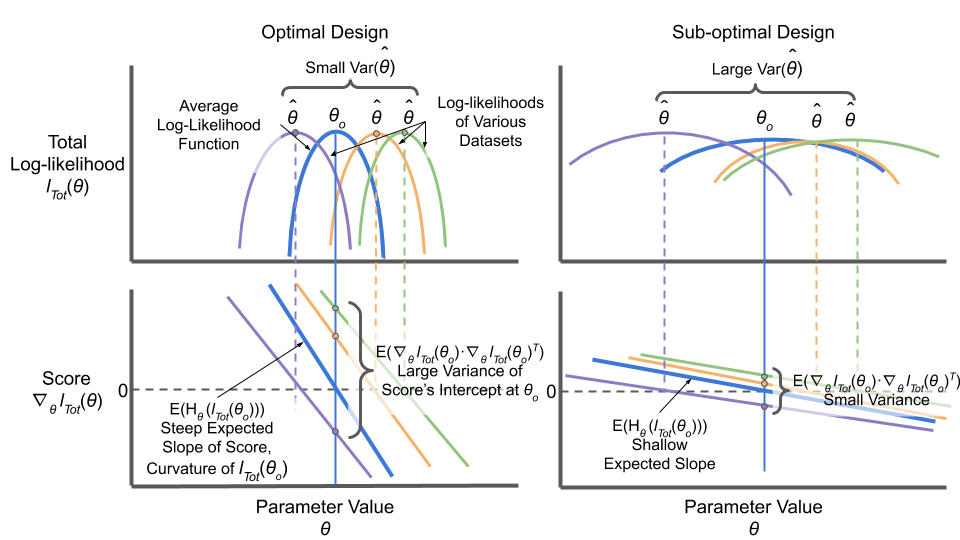
\includegraphics[scale=.4]{Images/FIM_diagram.png}
\caption{A figure comparing the total log-likelihood and score behaviour for multiple realizations of both an optimal design (left) and a sub-optimal design (right). The blue curves correspond to the average log-likelihood (top) and score function (bottom) for the given design -- averaged over all possible datasets. The other colors represent the log-likelihood and score functions for specific realizations of the design each with random observations.}
\label{fig:fim_diagram}
\end{figure}

The full proof of the FIM's connection to the parametric covariance is tedious and is not reproduced here, however it is possible to gain some intuition for how the FIM is linked to the covariance by observing some of its easily derived properties. By definition the maximum likelihood estimate occurs at the point, $\hat{\bm{\theta}}$, that maximizes $l_{Tot}(\bm{\theta})$. It follows that, at the optima, $\nabla_{\bm{\theta}}l_{Tot}(\hat{\bm{\theta}})=0$. Here the vector valued function $\nabla_{\bm{\theta}}l_{Tot}(\bm{\theta})$ is called the \textit{score}, and the MLE must occur at a point where all entries in the score are zero (due to first-order optimality conditions) \cite{pawitan2001all}. From the definition of the FIM, we see that it is the matrix of second moments and cross-moments for the score evaluated at our guess of the true parameter vector. It can be further shown asymptotically (at first-order) that the expected value of the score evaluated at the true parameter vector, $E_{\bm{y}_\mathcal{D}}[\nabla_{\bm{\theta}}l_{Tot}(\bm{\theta}_o)]$, is zero \cite{pawitan2001all}, which is consistent with the fact that the MLE is asymptotically non-biased.
%; regardless of which parameter vector makes the score zero for any given dataset, the score will be zero for the true parameter vector on average. Combing this with the definition of the FIM and the common decomp identity we have;
This expectation implies that the diagonal entries of the FIM are not just the second moments of the score, but the second central moments about its expected value, because
\begin{align}
\begin{aligned}
\text{Var}(\nabla_{\bm{\theta}}l_{Tot}(\bm{\theta}_o)) &= \text{diag}\{E_{\bm{y}_\mathcal{D}} [\nabla_{\bm{\theta}} l_{Tot}(\bm{\theta}_o) \cdot \nabla_{\bm{\theta}} l_{Tot}(\bm{\theta}_o)^T ]\} - E_{\bm{y}_\mathcal{D}}[\nabla_{\bm{\theta}}l_{Tot}(\bm{\theta}_o)]^2,\\ &= \text{diag}\{I_{Tot}(\mathcal{D},\bm{\theta}_o)\} - \bm{0}.
\end{aligned}
\label{eq:fim_var_score}
\end{align}
As the root of the score function fully defines the MLE, we should expect its variability to be strongly connected to the variability of the MLE estimate; in this case the variances are inversely related. If the variability of the score is large over multiple realizations of the experimental design, it implies that the estimate is heavily constrained by the design to fall near its expected true value. This scenario is depicted in Figure \ref{fig:fim_diagram} where, for the optimal design on the left, the intercepts of the individual score functions with the (blue) vertical line through the true parameter value, $\bm{\theta}_o$, exhibit large variability when the score functions' roots, $\hat{\bm{\theta}}$s, cluster around the true value. For the sub-optimal dataset on the right, the score function's value taken at the true parameter exhibits less variability and the estimates are therefore more variable.
%is strongly influenced by the data observed in a given realization of the design. This suggests that the estimate is very sensitive to the specific observations taken, and that the observations provide useful information for constraining the fitted parameter values, reducing the estimate's overall variability. 
%This is an intuitive leap, and a detailed connection between the score and estimate variability is made formal in the full proof (cite).

%This means that the FIM is equivalent to the MSE of the observed score about its expected value, providing some intuition for why the FIM is related to the MSE of the actual estimates. 

Intuition for the FIM can be developed further by expressing the FIM in an alternative form in terms of the log-likelihood's second derivatives. For an individual independent observation it can be shown that \cite{seber2003nonlinear}
\begin{align}
I_i(\bm{x}_j,\bm{\theta}_o) =  E_{Y_{i,j}} [\nabla_{\bm{\theta}} l_i(\bm{\theta}_o;y_{i,j},\bm{x}_j) \cdot \nabla_{\bm{\theta}} l_i(\bm{\theta}_o;y_{i,j},\bm{x}_j)^T ] =-E_{Y_{i,j}}[H_{\bm{\theta}}(l_i(\bm{\theta}_o;y_{i,j},\bm{x}_j))].
\label{eq:fim_hess}
\end{align}
Here $H_{\bm{\theta}}(.)$ is the Hessian operator with respect the parameter vector, such that the latter term above is the matrix of expected values of the second parametric derivatives of the log-likelihood. These two definitions of the FIM are equivalent under mild regularity conditions; to understand why, it is helpful to consider the single dimensional case. For a single observation $y$ and a single parameter $\theta$; the sampling probability is $p(y|\theta)$ and the log-likelihood is $l(\theta;y)=\log(p(y|\theta))$. Under mild regularity conditions, it follows from the identity $\int p(y|\theta)dy=1$ that $\int \frac{d}{d\theta}p(y|\theta)dy=0$ and $\int \frac{d^2}{d\theta^2}p(y|\theta)dy=0$ also hold. It then follows that \cite{lehmann2004elements}
\begin{align}
\begin{aligned}
E\left[\frac{d^2}{d\theta^2}l(\theta;y)\right] &= E\left[\frac{\frac{d^2}{d\theta^2}p(y|\theta)}{p(y|\theta)}\right] - E\left[\left(\frac{\frac{d}{d\theta}p(y|\theta)}{p(y|\theta)}\right)^2\right],\\
&= \int \frac{d^2}{d\theta^2}p(y|\theta) dy- \int \frac{\left(\frac{d}{d\theta}p(y|\theta)\right)^2}{p(y|\theta)} dy,\\
&= 0 - \int \left(\frac{d}{d\theta}l(\theta;y)\right)^2p(y|\theta) dy,\\
&= -E\left[\left(\frac{d}{d\theta}l(\theta;y)\right)^2\right].
\label{eq:1d_hess}
\end{aligned}
\end{align}

This result helps us to link the variance of the parameter estimate with the FIM -- defined as the variance of the score. To see this, note that while $E\left[\frac{d^2}{d\theta^2}l(\theta;y)\right]$ is a measure of the curvature of the log-likelihood, it is also the expected slope of the score function. This is shown in Figure \ref{fig:fim_diagram} where on the left, for the optimal design, the log-likelihood exhibits significant curvature around the optima; therefore the slope of the score, shown below, is very steep. On the right, the sub-optimal design has less curvature around the optima and therefore exhibits shallow slopes in the score below. It follows from the previous paragraph that, for the optimal design, given the diagonal entries of the FIM are large, the variance of the score's intercept with the vertical line at the true parameter value will be large. This also implies that the expected slope of those same score functions will be steep. With steep average slopes, the roots of the score functions will have a smaller variability. As the score's root is the MLE estimate, this implies the MLE has a lower variability in the optimal case. The situation is reversed for the sub-optimal design, where the low variability in the score's value at the true parameter and the score's shallow average slope allow the estimates to vary widely under multiple realizations of the design. These results also hold for multiple parameters and provide some intuition for connecting the FIM to the MLE's variability.
%In this relation it can be seen that when the expected curvature of the likelihood for a given design is large, the variability of the MLE will be small. This makes intuitive sense because if the log-likelihood exhibits significant curvature near its optima, it will result in a `pointy' optimization surface where small steps away from the optima in parameter space result in large decreases in the objective.
%BPI, figure for point blunt, top bottom plot, top plot with 'true' log-likelihood (infinite data) and various realized loglikelihoods (as quadratics), bottom plot with their corresponding scores, link is between the variance in the value of the realized scores at the true param, and the shape of the curvature of the loglikelihood in the top figure.
%On the other hand, when the curvature of the log-likelihood is small, the parameter estimate can exhibit wider variations from the optima with relatively little penalty in the objective. This implies that designs with large curvatures are less likely to allow random sampling errors to perturb the estimate significantly away from the expected true value.

As previously noted, we do not know the true value, $\bm{\theta}_o$, at which to take the asymptotic approximation and at which to evaluate the FIM. This means that any asymptotic results are inherently local to our nominal parameter vector, $\bar{\bm{\theta}}$. In practice initial estimates for $\bar{\bm{\theta}}$ can come from the available literature or from the MLE fit to some initial data. As the underlying model (i.e. $\bm{f}_i(.)$) must be sufficiently smooth, we can also expect asymptotic measures to hold approximately for parameter values near to the nominal vector. Other strategies have been proposed for dealing with the local nature of the FIM computed at the nominal parameter value $\bar{\bm{\theta}}$. Perhaps the most common approach is to implement optimal design in an iterative fashion, with each batch of optimized experiments adding to the collected data, improving the parameter estimates for the next round \cite{atkinson1992optimum}. In this case even though the designs are optimized for a local objective, the parameter estimates tend to become more accurate after each iteration. This accuracy is ensured by the increasing sample size, so even if the initial designs were erroneous and sub-optimal, as the estimates improve, so will the optimality of the iterative designs over the course of the experiment. However, some experimental contexts are not suitable for iterative design. In these case other strategies exist including Bayesian averaging over a parametric prior distribution or min-max optimization -- where the design is optimized for a parameter vector that has the worst estimation performance \cite{atkinson1992optimum,fedorov2010optimal}. In some cases, the local analysis alone can be useful if it is used to qualitatively explore optimal design structure under various parametric scenarios within the plausible parameter space; this has been done in some parts of this thesis.

%In cases where there exists no reasonable starting estimate, the asymptotic local measures can still be useful for exploring various scenarios within the plausible parameter space.
%BPI: add ref to global sensitivity tools here
%Asymptotic measures can also be used within a Bayesian framework to average results over a prior \cite{atkinson1992optimum}, however this work is outside the scope of this thesis.

Computing the derivatives and expectation required for the FIM for an arbitrary model may seem daunting. However, this derivation can be done quite simply by observing the following application of the chain rule \cite{fedorov2013optimal}:
\begin{align}
\begin{aligned}
\nabla_{\bm{\theta}} l_i(\bm{\theta};y_{i,j},\bm{x}_j) =& \nabla_{\bm{\theta}}  \log(p_i(y_{i,j}|\bm{\eta}_{i,j}{=}\bm{f}_i(\bm{x}_j,\bm{\theta}) )), \\
&\nabla_{\bm{\theta}} \bm{f}_i(\bm{x}_j,\bm{\theta}) \cdot \nabla_{\bm{\eta}_{i,j}} \log(p_i(y_{i,j}|\bm{\eta}_{i,j})).
\end{aligned}
\label{eq:chain_rule}
\end{align}
The above decomposition makes use of the fact that the sampling statistics, $\bm{\eta}_{i,j}$, of the observation distribution, $p_i(.)$, are directly computed by the deterministic model component such that $\bm{\eta}_{i,j}=\bm{f}_i(\bm{x}_j,\bm{\theta})$. The score function can therefore be decomposed into the deterministic model's parametric sensitivity and derivative of the log-probability of the observation with respect to the sampling statistics $\bm{\eta}_{i,j}$ \cite{fedorov2013optimal}. As the model sensitivity does not depend on the random observation values, $Y_{i,j}$, this simplifies the computation of the Fisher information matrix at each observation so that we have \cite{fedorov2013optimal}
\begin{align}
\begin{aligned}
I_i(\bm{x}_j,\bm{\theta}) &=  E_{Y_{i,j}} [ \nabla_{\bm{\theta}} \bm{f}_i(\bm{x}_j,\bm{\theta}) \nabla_{\bm{\eta}_{i,j}} \log(p_i(y_{i,j}|\bm{\eta}_{i,j})) \cdot \nabla_{\bm{\eta}_{i,j}}\log(p_i(y_{i,j}|\bm{\eta}_{i,j}))^T \nabla_{\bm{\theta}} \bm{f}_i(\bm{x}_j,\bm{\theta})^T ],\\
%&=   \nabla_{\bm{\theta}} \bm{f}_i(\bm{x}_j,\bm{\theta}) E_{y_{i,j}} [\nabla_{\bm{\eta_i}} \log(p_i(y_{i,j}|\bm{\eta_i})) \cdot  \nabla_{\bm{\eta_i}}\log(p_i(y_{i,j}|\bm{\eta_i}))^T] \nabla_{\bm{\theta}} \bm{f}_i(\bm{x}_j,\bm{\theta})^T  \\
&=   \nabla_{\bm{\theta}} \bm{f}_i(\bm{x}_j,\bm{\theta})~ \Psi(\bm{\eta}_{i,j}{=}\bm{f}_i(\bm{x}_j,\bm{\theta}))~\nabla_{\bm{\theta}} \bm{f}_i(\bm{x}_j,\bm{\theta})^T.
\end{aligned}
\label{eq:element_fim}
\end{align}
Here $\Psi(\bm{\eta}_{i,j}{=}\bm{f}_i(\bm{x}_j,\bm{\theta}))$ is defined as
\begin{align}
\Psi(\bm{\eta}_{i,j}{=}\bm{f}_i(\bm{x}_j,\bm{\theta})) = E_{Y_{i,j}} [\nabla_{\bm{\eta}_{i,j}} \log(p_i(y_{i,j}|\bm{\eta}_{i,j})) \cdot  \nabla_{\bm{\eta}_{i,j}} \log(p_i(y_{i,j}|\bm{\eta}_{i,j}))^T].
\label{eq:psi_fim}
\end{align}
This expectation is effectively just the Fisher information of a standard parametric distribution, such as the normal, Poisson etc., with respect to its sampling statistics. We follow Fedorov in referring to these matrices as elemental FIMs of the given distribution \cite{fedorov2013optimal}. These elemental FIMs have been computed for the vast majority of common one and two parameter distributions for which the expectation is analytically tractable. A good reference can be found in Fedorov's recent book \cite{fedorov2013optimal}. Therefore, computing the Fisher information for the overall experimental design, decomposes into computing a parametric sensitivity vector for each observation point, $\nabla_{\bm{\theta}} \bm{f}_i(\bm{x}_j,\bm{\theta})$, and matrix multiplying it with the observation distribution's elemental FIM; $\Psi(\bm{\eta}_{i,j}{=}\bm{f}_i(\bm{x}_j,\bm{\theta}))$. The formula for the elemental FIM for common parametric distributions is easily looked-up and computed from the predicted values of $\bm{\eta}_{i,j}$. The individual FIM's for each observation are then summed to produce the total FIM for the experiment. The total Fisher information matrix can be used to quantify the expected parameter estimate covariance for the given design at the nominal parameter values, $\bar{\bm{\theta}}$.

%Fisher originally derived results based on the Fisher information matrix to quantify the variability of parameter estimates, however it was later shown by Cramer and Rao that the inverse of the Fisher information matrix is also the lower bound for the variance of 

%Wald intervals and connection to FIM
%Without using higher order methods which are significantly more complicated (cite), approximating the bias, which is relevant for smaller sample sizes, generally requires simulation-based approximations via Monte Carlo methods. 
% Change ref to background in package chapter the nonlinear design book cite

% M J Box paper
% MSE, BIAS 
% JBS Haldane paper

\subsection{Scalar Objectives for Optimizing Designs}

%\textbf{Here we will start by discussing scalar objective functions computed from the FIM (i.e. alphabetic optimality criteria). We can mention how for some problems the optimization is convex if we optimize a relaxed design. We can mention some existing algorithms for design (Fedorov exchange algorithm) and the various trade-offs in posing the problem in convex or non-linear ways. We will especially mention tradeoffs in generating an exact design via optimization vs generating a relaxed design and rounding it.}

The Fisher information matrix captures approximate information about the expected distribution of the MLE estimate given a specified design. However, other than in the single parameter case, the Fisher information is matrix-valued which makes it unsuitable for use as an optimization objective. In order to construct an optimization problem for selecting an optimal design, we need a scalar function, $\Psi(.)$, of the FIM that can be maximized:
\begin{align}
\max_{\mathcal{D}} \Psi( I_{Tot}(\mathcal{D},\bar{\bm{\theta}}) ).
\label{eq:fim_hess}
\end{align}
The most common scalar objective in practice is the determinant of the Fisher information matrix \cite{atkinson1992optimum,fedorov2010optimal}. This is equivalent to minimizing the determinant of the expected covariance matrix of the parameter estimates. Optimizing a design subject to this objective is known as finding a D-optimal design \cite{atkinson1992optimum}. The determinant of a covariance matrix is referred to as the generalized variance of the underlying random vector, and as such the D-optimal design minimizes the generalized variance of the MLE estimate \cite{atkinson1992optimum}. The D-optimal design is commonly used because it has a number of useful properties, including that it is simple to compute, it can be formulated as a convex objective and D-optimal designs are invariant under re-parameterization \cite{atkinson1992optimum,fedorov2010optimal}. As such, D-optimal designs are the main designs studied in this work. Other than D-optimal designs, there exist a number of other scalar design criteria, these are sometime referred to as the alphabetic optimality criteria because they are generally named using single letters; for example, A-optimal, c-optimal, I-optimal etc. \cite{atkinson1992optimum}. 

%Ds objective, A objective, add them?
To find an optimal design, $\mathcal{D}$, we seek to find the optimal support points $\bm{x}_j\in\mathcal{X}$ and optimal replicate counts $\beta_{i,j}\in\mathcal{B}$.
Using a scalar objective, the overall optimization problem can be defined as
\begin{align}
\begin{aligned}
\max_{\mathcal{D}}~&\Psi(I_{Tot}(\mathcal{D},\bar{\bm{\theta}})),\\
I_{Tot}(\mathcal{D},\bar{\bm{\theta}}) &= \sum_j^N \sum_i^M \beta_{i,j} I_i(\bm{x}_j,\bar{\bm{\theta}}),\\
\mathcal{D}&=\{\mathcal{X},\mathcal{B}\}.
%\label{eq:tot_fim}
\end{aligned}
\end{align}
This optimization is difficult for a number of reasons. It is non-linear in the support points, $\bm{x}_j$. It is also an integer programming problem because of the integer restrictions on $\beta_{i,j}$. Also, the optimal number of support points, $N$, is not generally known. These computational difficulties are already layered on top of those required to compute the FIM, as the FIM also requires computing sensitivities, which can be difficult for certain models.

A common approach for reducing the computational difficulty of optimal design is to relax the integer constraint such that a continuous weighting, $\xi_{i,j}$, over the input-observation pairs is optimized \cite{atkinson1992optimum}. In this relaxed formulation, each $\xi_{i,j}$ replaces the corresponding $\beta_{i,j}$, however the $\xi_{i,j}$ have non-negative real-values which are constrained so that $0<\xi_{i,j}<1$ and $1=\sum_i^M \sum_j^N \xi{i,j}$. For a relaxed design the replicate weights, $\xi_{i,j}$, are grouped in the weight set such that $\xi_{i,j}\in\mathcal{Z}$. A relaxed design, $\mathcal{D}_R$, is then defined by the support points and weight set such that 
$\mathcal{D}_R=\{\mathcal{X},\mathcal{Z}\}$. The relaxed optimization problem can then be written as
\begin{align}
\begin{aligned}
\max_{\mathcal{D}_R}~&\Psi(I_{Tot}(\mathcal{D}_R,\bar{\bm{\theta}})),\\
I_{Tot}(\mathcal{D}_R,\bar{\bm{\theta}}) &= \sum_j^N \sum_i^M \xi_{i,j} I_i(\bm{x}_j,\bar{\bm{\theta}}),\\
\mathcal{D}_R&=\{\mathcal{X},\mathcal{Z}\}.
%\label{eq:tot_fim}
\end{aligned}
\end{align}
An exact design, $\mathcal{D}$, specified using integer replicate allocations, $\beta_{i,j}$, can be converted to a relaxed design, $\mathcal{D}$, by dividing the replicate integers by the total sample size: $\beta_{i,j}/N_{Tot}=\xi_{i,j}$. The total FIMs, $I_{Tot}$, of the two design representations are therefore also related by the sample size so that $I_{Tot}(\mathcal{D},\bar{\bm{\theta}})/N_{Tot}=I_{Tot}(\mathcal{D}_R,\bar{\bm{\theta}})$. Given these relations, the relaxed formulation is effectively normalized so that it does not depend on the overall sample size, $N_{Tot}$. To convert a relaxed design, $\mathcal{D}_R$, to an implementable exact design, $\mathcal{D}$, with integer replicate allocations, a sample size is selected and a rounding procedure is then applied to generate $\beta_{i,j}$ from the weights $\xi_{i,j}$. Simple rounding or specialized apportionment methods can be used for this conversion \cite{pukelsheim1992efficient,wilhelm1996obtain,imhof2001efficiencies}. Due to the computational advantages, the relaxed form of the design problem is used for optimization throughout this thesis. 
 
After solving the full design optimization problem, or the relaxed approximation to it, the research will achieve an optimal design with a specified list of support points and replicate allocations. This design will be optimal in a mathematical sense, but only conditionally for the given model structure, nominal parameter values, observation distributions and experimental constraints the research has specified. It is important to remember that optimal designs are generated under these strong assumptions. This means that other sources of uncertainty about model structure and alternative sources of variability are not necessarily hedged for in the optimized design. The optimal design can therefore serve as an idealized guide for a given system, however the design should be combined with good experimental judgment when implementing the prescribed measurements in practice.


%When addressing the relaxed version of the problem, 
%mention the GET and what it appleis (convex objective and relaxed weights)
%local, iterative, bayesian, min-max


%%%%%%%%%%%%%%%%%%%%%%%%%%%%%

%An optimized design with a large sample size will desensitize the the estimate to the sampling error, concentrating the estimate's distribution near the true value.

%Here there are $N_y$ observation variables, indexed by $j$, and $N_x$ support points $\bm{x}_i$, indexed by $i$. The FIM at a given input point, $\bm{x}_i$, for the $j$th observation variable $y_j$ is $\mathcal{I}_j(\bm{x}_i)$. The weights $\beta_{ij}$ correspond to the support point $\bm{x}_i$ and the observation variable $y_j$. The collection of weights, $\beta_{ij}$,

%Connection to cramer rao lower bound Fisher derived the fim as an approximate to an estimators variance, Cramer and Rao later showed that creates a lower bound for teh variance of an unbiased estimator, this is less useful in thinking about it as a method for experimental design

 %The MSE can be  The MSE, covariance and bias each contain useful and intuitive information about parameter estimation error. 
 %However, these metric can be approximated, either asymptotically or through simulation at a candidate point (i.e. an guess or estimate) for the true parameter vector. The \texttt{evaluate()} function provides both types of methods for computing these metrics for a given design, given a nominal true value.

%The \texttt{evalutate()} method implements a parametric Monte Carlo algorithm for approximating the MSE, covariance and bias terms. In this method, a 'true' nominal parameter vector is used to simulate a large number of datasets corresponding to the candidate design. These datasets are then each fit independently using maximum likelihood. The resulting set of estimated parameter vectors are then used to compute the MSE, covariance and bias empirically, using the nominal parameter value as a stand-in for the unknown true value. This then provides an approximation for the parameter accuracy metrics for the given design. The Monte Carlo approximation is time consuming and the sample number used may need to be tuned to the design and model begin evaluated in order to achieve stable approximations, as the algorithm necessarily is non-deterministic. These considerations make the Monte Carlo approach unsuitable for use in the \texttt{Design} optimization, however they are useful benchmarks to assess the suitability of asymptotically derived designs at small sample size. The Monte Carlo metrics are also valuable for comparing amongst several design candidates, allowing the user to accurately differentiate between subtle trade-offs in bias and variance components of parameter error. 

% \paragraph{Confidence Intervals}

% likelihood-based intervals \cite{seber2003nonlinear,bates1988nonlinear} (cite check). (While both likelihood-based and Wald intervals --computed from the FIM-- have asymptotic justifications, likelihood-based intervals require observed data where as Wald intervals do not \cite{seber2003nonlinear,bates1988nonlinear} (cite check).)(i.e. if the experiment was repeated 100 times, 95 of the computed estimates would have a smaller difference)

%Asymptotic computation of the parameter accuracy metrics is done for a specific fitting method. Here we focus on the maximum likelihood estimate, which is the fitting method implemented in the \texttt{fit()} function of the \texttt{Model} class. 

% \paragraph{Asymptotic Properties}


% Cite paper by JBS Haldane on higher order sampling distributions in paranthetical (ask brian about story/book he got it from)

% The goal in experimental design is to evaulate a designs expected performance before the experiment is even run.

% The full bayesian integral is set up as follows
% \begin{align}
% \begin{aligned}
% \int math stuff
% \end{aligned}
% \label{eq:full_objective}
% \end{align}
% (this doesn't even get into model uncertainty or input settings errors)

% In practice this is intractable for all but the simplist models, to simplify there are several options.

% Parameteter integral can be replaced by a point estimate, an initial guess essentially. The whole procedure can also be applied iteratively, where the total numbe of samples are divided up in the hopes that after each round of expeirmention the parameter fit will improve, providing a more accurate starting point for the next round of optimization (no proofs are knonw to the authour guaranteeing that this process will always converge even for the 

%\paragraph{Fisher Information}

%\paragraph{Approximate vs Exact Designs}


\section{Package Workflow and Definitions}

The NLOED package is written in Python 3 and can be used in Python scripts or interactively in the interpreter. The package consists primarily of two core classes; the \texttt{Model} class and the \texttt{Design} class. The \texttt{Model} class encodes information about model structure, observation distributions, and model-specific functions such as those used for fitting, simulation and model analysis. The \texttt{Design} class accepts models and other design information and can be used to optimize and output experimental designs. 

Model equations passed into the \texttt{Model} class are created using CasADi symbolics and the CasADi \texttt{Function} class. Use of CasADi constructs enables much of the auto-generated functionality within the main two classes. Due to this reliance on CasADi, the core package does require some familiarity with model construction in the CasADi framework. However the modular and object-oriented nature of the core package classes means it is amenable to future extensions, such as wrapping the core classes in more beginner-friendly helper functions or GUI interfaces.

Output from both the \texttt{Model} and \texttt{Design} classes is primarily returned as Pandas and Numpy data structures. For examples experimental designs, model simulations and predictions are exported as Pandas dataframes. Data, candidate designs, and other user provided information are also passed into class functions as dataframes. This makes it easy to read in raw data from Excel and CSV files, via Pandas functions like \texttt{read\_csv()}, \texttt{to\_csv()}, \texttt{read\_excel()} and \texttt{to\_excel()}. The use of dataframes also makes it easy to plot model predictions and sample data using third-party plotting packages such as Matplotlib, as well as exporting output to a variety of formats for use in other tools such as MATLAB and R.

% \begin{itemize}
%   \item Package is written in Python and accessed programmaticly
%   \item Package consists of 2 core classes 'Model' for code associated with model construction and use, and 'Design' for generating experimental designs from a Model or list of Models
%   \item Models are coded in Casadi symbolics (shorten:The packages is written and accessed in Python and makes extensive use of CasADi's symbolic framework at both the user interface level, where the user defines models in Casadi symbolic, and under the hood, where it is used for senstivity analysis, FIM computation and optimization. Due to this heavy reliance on Casaid, the core package does require some familiarity with model construction in Casadi, however the modular and object-oriented nature of the core package classes means it is amenable to future extensions that may wrap the core classes in more beginner-friendly helper functions or GUI interfaces. )
%   \item Output is generated in the form of Pandas and Numpy data structures, this is convenient for many reasons (shorten: The packages interfaces naturally with other standard numerical and data process Python libraries such as Pandas and Numpy. For examples experimental designs, data and predictions are imported and exported as Pandas dataframes. This makes it easy to read in raw data from excel and CSV files. It also makes it easy to plot model predictions and sample data using third party plotting software such as Matplot lib, as well as exporting to a variety of formats, or calling other Python libraries or exprting to Matlab and R.)
% \end{itemize}

%\subsection{Basic Workflow}
\begin{figure}[htb!]
\centering
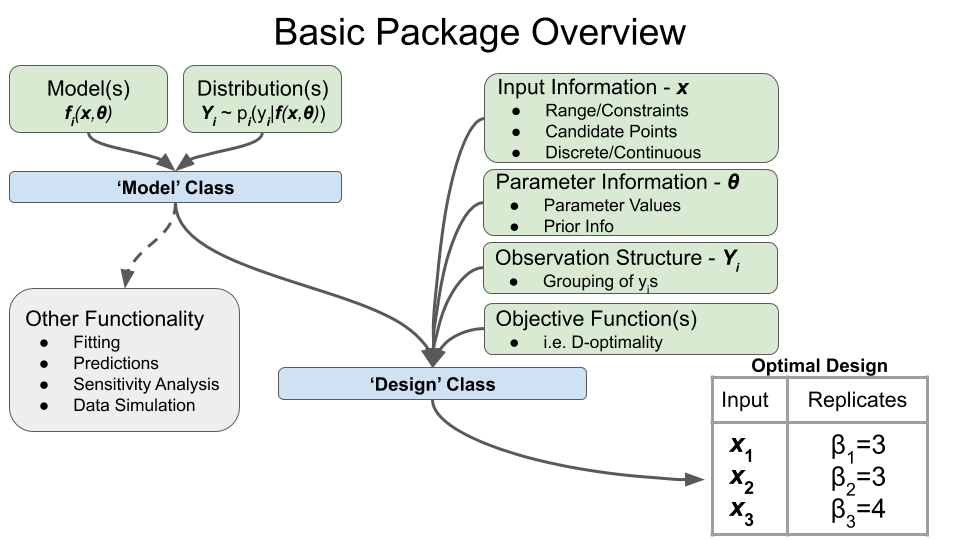
\includegraphics[scale=.4]{Images/PackageOverview.png}
\caption{A diagram depicting the archetypal NLOED workflow including model creation using the \texttt{Model} class, and design creation using the \texttt{Design} class. Here $\bm{x}$ is the vector of model inputs describing the experimental conditions, $\bm{y}$ are the observation variables, $\bm{\theta}$ are the unknown model parameters, $\bm{f}(.)$ is the model function and $p(.)$ is the data distribution, see text for further description.}
\label{fig:workflow}
\end{figure}
The majority of use cases for the package center around a simple archetypal workflow, as shown in Fig. \ref{fig:workflow}: 1) \textit{Model creation}; create a model using CasADi symbolics and the NLOED \texttt{Model} class, 2) \textit{Design creation}; pass the \texttt{Model} instance, along with other design specifications, into the \texttt{Design} class constructor to create an optimal design. This simple pattern can be recycled in a variety of ways, i.e. to construct simulation studies, to compare designs across different models, or to generate design variations with a single model. The \texttt{Model} class can perform a range of other functions, such as fitting and simulation, which are useful in both real experimental work and simulation studies.

\subsection{Model Definition} 

Before discussing the programmatic details of model creation in the NLOED package, we first define what mathematical structure NLOED accepts as a suitable model. NLOED models generally follow the model specification given in Chapter \ref{background_chapter}, which is briefly reviewed here. The model connects the random  observation variables, $Y_i$, with model input vector, $\bm{x}$, which quantifies the experimental conditions. Note that when considering the model declaration the user can ignore the $j$ sub-scripting on the input vectors, $\bm{x}_j$, as the number of unique experimental conditions is not addressed until the design phase. Therefore, when not discussing the data or a design, it is often convenient to suppress the $j$th index on $\bm{x}_j$, $\bm{\eta}_{i,j}$, $Y_{i,j}$ and $y_{i,j}$.
%Recall that each $Y_i$ represents a given type of observation but the actual random variable is properly sub-scripted as $Y_{i,j}$ because the $i$th observation variable, $Y_i$ always has the same, possibly unique, type of distribution, $p_i(.)$, but its shape is conditional on $j$th input, $\bm{x}_j$. 
Recall that each $Y_i$ is a random variable representing a given type of observation. Each $Y_i$ has a specific parametric distribution, $p_i(.)$, but this distribution's shape is conditional on the model inputs $\bm{x}$ and the unknown parameter vector $\bm{\theta}$.
Therefore for each possible observation, $Y_i$, the connection between input and observation is mediated by two components: 1) the conditional observation distribution, $p_i(y_i|\bm{\eta}_i)$ and 2) the deterministic model function $\bm{\eta}_i=\bm{f}_i(\bm{x},\bm{\theta})$. These two components are combined to create the overall model:
\begin{align}
Y_i \sim p_i(y_i|\bm{\eta}_i{=}\bm{f}_i(\bm{x},\bm{\theta})).
\label{eq:model_def_repeat}
\end{align}
The observation distributions, $p_i(.)$, in NLOED are all parametric distributions and they currently include; the normal, Poisson, binomial, log-normal, Bernoulli, exponential and gamma distributions. The deterministic model, $\bm{f}_i(.)$, maps the experimental conditions $\bm{x}$ to the sampling statistics, $\bm{\eta}_i$, of the observation distribution $p_i(.)$. The function $\bm{f}_i(.)$ must be sufficiently smooth and implementable in CasADi symbolics. This permits a wide range of model types including models based on numerical integration. Recall the sampling statistics are the natural parameters of the parametric distribution $p_i(.)$. For example with the normal distribution the sampling statistics are the mean and variance, for the Poisson distribution the sampling statistic is the $\lambda$ rate parameter, and for the Bernoulli distribution the sampling statistic is the probability of a success. Therefore in NLOED the model function $\bm{f}_i(.)$ does not always predict the mean observational response, but rather predicts the appropriate sampling statistics of the random variable, $Y_i$, assigned to the given observation type. Specifying models in this way allows for much more flexibility in the types of experimental observations NLOED can handle. Each $y_i$ represents a single-dimensional realization of the random observation variable $Y_i$. NLOED always assumes all observation variables $Y_i$ are independent; this allows NLOED to easily accommodate a variety of distribution types rather than only supporting (possibly correlated) normally distributed data. When creating a model in NLOED the user must specify the vector dimensions of the parameters, $\bm{\theta}$, and of the model inputs, $\bm{x}$, as well as the list of observation variables, $Y_i\in\bm{Y}$. The user must also indicate the distribution type of $p_i(.)$ for each observation variable, $Y_i$, and they must provide the model function, $\bm{f}_i(.)$ using CasADi's symbolic tools. The distribution, $p_i(.)$, and the function $\bm{f}_i(.)$ for each $Y_i$ are passed as a list so the user can add as many observations as is desired.

% Before discussing the programmatic details of model creation in the NLOED package, we first define what mathematical structures NLOED accepts as a suitable model. % Here we formalise what a model is defined as for use in NLOED's \texttt{Model} class. 
% %The first step of model building consists of collecting relevant information concerning the model in the \texttt{Model} class instance. 
% NLOED models consists of two components, the deterministic mathematical model and the error distribution of the observations. 

% Systems biologists are likely quite familiar with the deterministic component of their models, however the sampling distribution may be less familiar. However, the sampling distribution is important for maximum likelihood fitting as well as for computing the Fisher information. A mathematical description of a simple one-dimensional NLOED model is shown in Eq. \ref{eq:nloed_model_def}.
% \begin{align}
% \begin{aligned}
% \bm{\eta}_i &= \bm{f}_i(\bm{x},\bm{\theta})\\
% y_i &\sim p_i(y_i|\bm{\eta}_i)
% \end{aligned}
% \label{eq:nloed_model_def}
% \end{align}
% %BPI: independence is typically assumed, but seems like a big assumption to hard-code, no? (also typo: joint’)
% \noindent Here $\bm{x}$ represents a vector of experimental inputs the user can control. The vector $\bm{\theta}$ contains the parameter vector of values to be estimated in the experiment. The function $\bm{f}_i(.)$ maps the experimental inputs, $\bm{x}$, and parameters, $\bm{\theta}$, to the deterministic output vector $\bm{\eta}_i$. Here the model specification is somewhat more general than some users may be used to, as the output vector $\bm{\eta}_i$ consists of, what we refer to as, the \textit{sampling statistics} of the observation variable $y_i$. 
% %BPI: sampling statistics will need a gentle introduction. Suggest breaking this out into its own paragraph (with the example below)
% The observation $y_i$ is a one-dimensional observation generated from the model which is drawn from the error distribution $p_i(.)$. Here the subscript $i$ indicates the observation variable in general, not an individual realization from the distribution. Generally a unique, observation variables, $y_i$, is used for each different measurement taken of the system, including measurements of the same quantity at different points in time or space. The error distributions in the NLOED package are confined to parametric families including the normal, Poisson, binomial, Bernoulli, exponential, gamma and log-normal distributions.
% %BPI: including? are there more?
% (The sampling statistics $\bm{\eta}_i$ could be referred to as the distributional parameters of $p_i(.)$, however we wish to avoid confusion with the model parameters $\bm{\theta}$.) Thus if the user assumes $y_i$ comes from normal distribution with a fixed known variance (equivalent to least squares fitting), then $\bm{\eta}_i$ consists of the mean of the observations, $\mu_i$, and their variance, $\sigma_i^2$, such that $\bm{\eta}_i=[\mu_i,\sigma_i^2]$. In this case, the function $f_i(\bm{x},\bm{\theta})$ maps the given model inputs and parameters to the model mean $\mu$ and a fixed constant for the variance $\sigma^2$. In the normally distributed case, the sampling statistics $\bm{\eta}_i$ is vector valued (two-dimensional), however other parametric families, such as the exponential or the Poisson distribution have one-dimensional sampling statistics. Also the model function $\bm{f}(\bm{x},\bm{\theta})$ must be encoded in CasADi symbolics, this permits a wide range of model types including models based on implicit functions or numerical integration. However models must be differentiable and therefore $f(\bm{x},\bm{\theta})$ cannot contain discontinuities, \texttt{if/else} statements or any random sampling (i.e. stochastic models computed using a random algorithm).

% The description given in equation \ref{eq:nloed_model_def} is for a single observational dimension, mapping multiple inputs to a single observation variable. NLOED models are designed to by multi-input and multi-output and so a full model instance will often contain a list of observation variables and their associated models. Equation  \ref{eq:nloed_model_vec} formalizes this notion in a vectorized version of the one-dimensional example.
% %BPI: A figure of this scenario would be nice here
% \begin{align}
% \begin{aligned}
% \bm{H} &= \bm{F}(\bm{x},\bm{\theta})\\
% \bm{Y} &\sim \bm{P}(\bm{Y}|\bm{H})
% \end{aligned}
% \label{eq:nloed_model_vec}
% \end{align}
% \noindent Here $\bm{Y}$ is a vector of observations variables the model can generate such that $\bm{Y}=[y_1,...,y_N]$. Each of these observations $y_i$ is drawn from a distribution $p_i(.)$, which can be of varying types within the same overall model. Observations are assumed to be independent in the NLOED package so that the join distribution of each unique observation $\bm{P}$ is simply the product of the individual distributions i.e. $\bm{P}(\bm{Y}|\bm{H})=\prod_i p_i(y_i|\bm{\eta}_i)$. The matrix $\bm{H}$ consists of the individual sampling statistics $\bm{\eta}_i$ for each distribution $p_i(.)$. (We use the term matrix here loosely, as each set of sampling statistics $\bm{\eta}_i$ can have either one or two elements depending on the distribution.) Likewise, the function vector $\bm{F}$ consists of set of deterministic deterministic functions, such that $\bm{F}(\bm{x},\bm{\theta})=[\bm{f}_1(\bm{x},\bm{\theta}),...,\bm{f}_N(\bm{x},\bm{\theta})]$. This list of functions maps inputs $\bm{x}$ and parameters $\bm{\theta}$ to the sampling statics $\eta_i$.
% Here each $y_i$ corresponds to a unique observation type and thus does not include replicates; this implies each $y_i$ has a unique function $f_i$ and a unique conditions distribution $p(y_i|\bm{\eta}_i)$.
\begin{figure}[htb!]
\centering
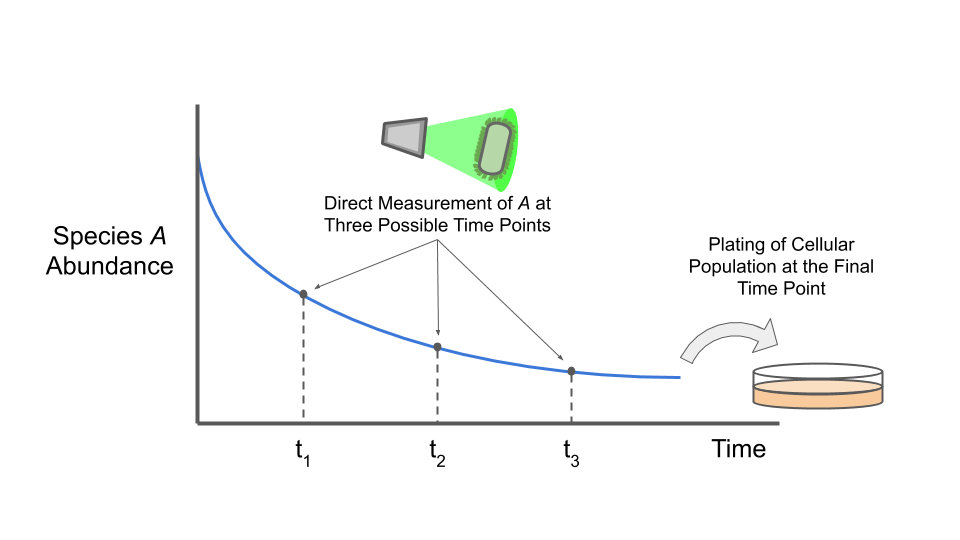
\includegraphics[scale=.4]{Images/example_experiment.png}
\caption{A figure depicting an example experimental scenario, involving a decaying cellular species $A$. The experiment includes both direct measurement of $A$ and a plate count assessing $A$'s potential for conferring resistance to a selective agent.}
\label{fig:example_model}
\end{figure}
Specifying models in this way provides flexibility in mixing different observation types. As an example, assume synthesis of a biochemical species $A$ has previously been induced in a cell culture and $A$'s intra-cellular concentration is undergoing exponential decay. This scenario is depicted in Figure \ref{fig:example_model}. An experimenter wishes to take some replicate measurements of $A$ at any of three possible time points spaced evenly throughout the first three hours after decay begins. Furthermore, assume that $A$ confers some selection resistance and the experimenter will plate the culture on selective plates at the fourth hour and perform a plate count. Assume the experimenter controls the initial induction level as input $x_1$. In this proposed experiment there are four observation variables; $Y_1$, $Y_2$, and $Y_3$ are observations of $A$'s concentration at one, two and three hours after induction. Observation $Y_4$ is the plate count from the fourth hour. We assume that $p_1(.)$ $p_2(.)$, and $p_3(.)$ are normally distributed with a known fixed variance of $\sigma^2=1$, and $p_4(.)$ is Poison distributed. We assume that the mean concentration of $A$ can be modelled as
\begin{align}
\mu(t)=\alpha x_1 e^{-\gamma t},
\end{align}
 we assume that the Poisson rate for the plate count is modeled as
\begin{align}
\lambda(t) =  \frac{\nu}{\frac{\kappa e^{\gamma t}}{\alpha x_1} +  1}.
\end{align}
 The model can be defined by listing out the model components as:
 %in Fig. \ref{eq:nloed_model_examp}.
% \begin{align}
% %\begin{aligned}
% \bm{x} = [x_1],~
% \bm{\theta}=[\alpha,\gamma,\nu,\kappa]\\
% p_1(.)=\text{Normal},~p_2(.)=\text{Normal},~p_3(.)=\text{Normal},~p_4(.)=\text{Poisson}]\\
% \bm{\eta}_1=[\mu(1),\sigma^2],~\bm{\eta}_2=[\mu(2),\sigma^2],~\bm{\eta}_3=[\mu(3),~\bm{\eta}_1\sigma^2],~\bm{\eta}_4=[\lambda(4)]]\\
% ~\bm{f}_1(\bm{x},\bm{\theta})= \Bigg[\alpha x_1 e^{-\gamma },1\Bigg],~\bm{f}_2(\bm{x},\bm{\theta})=\Bigg[\alpha x_1 e^{-2\gamma },1\Bigg],\\
% \bm{f}_3(\bm{x},\bm{\theta})=\Bigg[\alpha x_1 e^{-3\gamma },1\Bigg],~\bm{f}_4(\bm{x},\bm{\theta})=\Bigg[ \frac{\nu}{\frac{\kappa e^{4\gamma }}{\alpha x_1} +  1}\Bigg]
% %\end{aligned}
% \label{eq:nloed_model_examp}
% \end{align}
\begin{align}
\begin{aligned}
&\bm{x} = [x_1],~&&\bm{\theta}=[\alpha,\gamma,\nu,\kappa],~&&\bm{Y}=[Y_1,Y_2,Y_3,Y_4]\\
&p_1(.)=\text{Normal},~&&\bm{\eta}_1=[\mu(t{=}1),\sigma^2],~&&\bm{f}_1(\bm{x},\bm{\theta})= \left[\alpha x_1 e^{-\gamma },1\right]\\
&p_2(.)=\text{Normal},~&&\bm{\eta}_2=[\mu(t{=}2),\sigma^2],~&&\bm{f}_2(\bm{x},\bm{\theta})=\left[\alpha x_1 e^{-2\gamma },1\right]\\
&p_3(.)=\text{Normal},~&&\bm{\eta}_3=[\mu(t{=}3)\sigma^2],~&&\bm{f}_3(\bm{x},\bm{\theta})=\left[\alpha x_1 e^{-3\gamma },1\right]\\
&p_4(.)=\text{Poisson},~&&\bm{\eta}_4=[\lambda(t{=}4)],~&&\bm{f}_4(\bm{x},\bm{\theta})=\left[ \frac{\nu}{\frac{\kappa e^{4\gamma }}{\alpha x_1} +  1}\right].
\end{aligned}
\label{eq:nloed_model_examp}
\end{align}
%(Could discuss how time could be treated as an input and out DE's work but best to keep it simpler here, perhaps simplify)

Another possible model structure for this experimental scenario would involve treating the observation time for the $A$ species assay as a second input dimension, $x_2$. In this scenario there would now be only two observation variables: $Y_1$ is the abundance of species $A$ at any time point before the fourth hour, and $Y_2$ is the plate count performed at the fourth hour. Using this encoding the model structure would be
\begin{align}
\begin{aligned}
&\bm{x} = [x_1,x_2],~&&\bm{\theta}=[\alpha,\gamma,\nu,\kappa],~&&\bm{Y}=[Y_1,Y_2]\\
&p_1(.)=\text{Normal},~&&\bm{\eta}_1=[\mu(t{=}x_2),\sigma^2],~&&\bm{f}_1(\bm{x},\bm{\theta})= \left[\alpha x_1 e^{-\gamma x_2},1\right]\\
&p_2(.)=\text{Poisson},~&&\bm{\eta}_2=[\lambda(t{=}4)],~&&\bm{f}_2(\bm{x},\bm{\theta})=\left[ \frac{\nu}{\frac{\kappa e^{4\gamma }}{\alpha x_1} +  1}\right].
\end{aligned}
%\label{eq:nloed_model_examp}
\end{align}
\noindent This encoding provides greater flexibility in the sampling schedule of $A$ which may be desirable or problematic depending on the experimental protocol.
Choosing the appropriate encoding for a given experimental scenario depends on practical aspects of the protocol and numerical considerations for the optimization. Information and examples provided throughout this chapter will be useful for guiding this decision.
Regardless of how the model is encoded, specification of the deterministic model components and the observation distributions fully defines an NLOED model.
%Note that in defining the model the user does not enter specific parameter values, these are handled at the design phase.
Receiving this information, the \texttt{Model} class constructor auto-generates a large variety of useful code including maximum likelihood fitting functions, parametric sensitivity functions, and model prediction and sampling functions as described below.
%\begin{itemize}
  %\item The primary components of a package model are i) a deterministic function linking inputs and parameters to sampling statistics, ii) a sampling distribution that describes the observation variability.
  %\item equation maybe??
  %\item Models can contain multiple observations, and thus multiple deterministic components and and distributions. For example normally distributed measurments of mean culture data, along with plate count poisson, and binomial responses etc.
  %\item The Model class encapsulates the model structure, from this it can be used to autogenerate many useful features (ML fitting, sensitvity and prediction uncertainty etc.). But doesn't store any parameter value information, this data is handled primarily by the user.
  %\item As an example the user may have a model structure and some data from preliminary expderiments. They would encode the model and use the Model fitting feature to get a preliminary data 
%\end{itemize}

\subsection{Design Definition}

Designs in NLOED generally follow the design definition outlined in Chapter \ref{background_chapter}, which is summarized here for convenience. Designs in NLOED must specify two main pieces of information, 1) the set of input conditions (support points) $\bm{x}_j\in\mathcal{X}$ used in the experiment and 2) the number of replicate observations $\beta_{i,j}\in\mathcal{B}$ taken of each observation variable, $Y_i$, in each condition $\bm{x}_j$. These two properties are common to most design formalisms  \cite{atkinson1992optimum,fedorov2013optimal}. NLOED uses two different types of designs in its workflow; \textit{relaxed designs} and\textit{exact designs} (see Chapter \ref{background_chapter} for further discussion). In exact designs, each $\beta_{i,j}$ is an integer and the overall sample size for the experiment, $N_{Tot}$, is the sum of the replicates in each observation and in each condition: $N_{Tot}=\sum_j^M\sum_i^N \beta_{i,j}$. Relaxed designs instead use real valued weights, $\xi_{i,j}$, between $0$ and $1$ to represent the replicate allocations to each observation and in each condition.  The sum of the real valued weights is $1$ and therefore relaxed designs do not have a sample size. Instead the weights represent the approximate fraction of an arbitrary sample size that should be allocated to each input and observation condition so that $N_{Tot}\xi_{i,j}\approx \beta_{i,j}$. This relation only holds approximately because the weights, $\xi_{i,j}$, may not share the desired sample size as a common denominator, or may even be irrational. NLOED uses both design types in its workflow because it generates designs using an optimize-then-discretize approach. Initially an optimal relaxed design is solved for, after which the relaxed design is then rounded to a discrete exact design with a desired sample size. Optimizing the exact design directly is difficult because, with $\beta_{i,j}$ restricted to discrete integers, the resulting optimization problem is a nonlinear integer programming problem which is difficult to solve efficiently \cite{atkinson1992optimum,fedorov2013optimal}. The term \textit{relaxed} comes from the relaxation of the integer constraint. Relaxed designs can be viewed as a mathematical idealization of an optimal experiment with infinite data which means they can be difficult to implement with small finite sample sizes \cite{atkinson1992optimum,fedorov2013optimal}. %Exact designs on the other hand, specify exactly how many discrete replicates are taken in each condition, and thus are suitable for use in real experimental settings\cite{atkinson1992optimum,fedorov2013optimal}.
 %As a result, the \texttt{Design} class finds and stores this relaxed design internally after instantiation. 
%Relaxed designs are created when the user instantiates a \texttt{Design} class instance. The resulting \texttt{Design} object then stores an archetypal relaxed solution to the problem within its class data.

While an approximation, the optimize-then-discretize approach naturally splits the workflow into two phases providing greater flexibility for the user. Specifically, the user's ultimate goal may be to choose their sample size to achieve certain accuracy objectives as efficiently as possible; they wish to take as few samples as they can but as many as they must. An optimal design will help to improve estimation accuracy, however the overall sample size is a more important factor. The accuracy of parameter estimates always improves monotonically with increasing sample size and the structure of the design only determines how much marginal improvement each additional measurement contributes. When optimizing an exact design directly the user must specify the sample size before they optimize, which means they do not know the structure or the pre-factor utility of the optimal design when the overall size of the experiment is chosen.
%Often the user may have a rough upper bound for their overall sample size but they are much more concerned with making efficient use of each unit of experimental effort.
Therefore, in direct optimization of the exact design, choosing a minimally sufficient sample size would require multiple runs of a difficult integer programming problem. By optimizing the relaxed design first, the user will achieve an approximately optimal design structure. They can then use efficient rounding procedures to investigate multiple sample sizes and choose the lowest possible experimental burden that achieves their desired accuracy level. 

%While approximate, the optimize-then-discretize approach does provide some advantages. The relaxed optimization is much faster and more efficient than nonlinear integer programming, improving turnaround and confidence that at least a local optima has been found. Also, 

%In the optimize phase the user generates a relaxed design that sets the structure of the optimal experiment and then the sample size is selected during the rounding procedure. 
%This creates a natural workflow where the user can use the model alone to derive an optimal design archetype, and then tune the sample size to achieve their desired performance.  Often this fits well with other experimental considerations in that the user may have a rough upper bound for their overall sample size but is much more concerned with making efficient use of each unit of experimental effort and may wish to vary their sample size to achieve certain accuracy objectives efficiently. 
%The process of rounding relaxed designs is not entirely trivial, especially at small sample sizes, and the process of rounding can result in some lose of optimality.
%Not all relaxed designs result in continuous weights that can be exactly preserved for arbitrary integer sample sizes, in fact most rounding procedures do not results in an exact design that exactly replicates the fractional weights of the relaxed design when normalized by the sample size.
%and a truly optimal design at the exactly specified sample size may require some readjustment of the support points or even the addition of new support points. This is especially exacerbated when the user seeks exact designs with small sample sizes, where the small size significantly restricts the range of achievable weightings. 
%However, despite these difficulties, the rounding process does provide some advantages.


%the relaxed optimization is much faster and more efficient than nonlinear integer programming, improving turnaround and confidence that at least a local optima has been found. The relaxed design is also archetypal for the model in that its design represents the best possible allocation of resources in idealized conditions. The performance of the relaxed design is an upper bound for what can be achieved. This can be useful as a feasibility check on identifiability early in model development.
%Perhaps most importantly, the division of the design process into optimization and rounding naturally splits the design into two phases. The optimization sets the structure of the optimal experiment and then the sample size is selected during the rounding procedure. The final accuracy of parameter estimates can be improved monotonically by increasing the sample size, but the design influences how much marginal improvement each additional measurement contributes. This creates a natural workflow where the user can use the model alone to derive an optimal design archetype, and then tune the sample size to achieve their desired performance.  Often this fits well with other experimental considerations in that the user may have a rough upper bound for their overall sample size but is much more concerned with making efficient use of each unit of experimental effort and may wish to vary their sample size to achieve certain accuracy objectives efficiently. 

\begin{table}
\centering
\caption{An example of the structure used to represent an experimental design in the NLOED package. Here both the continuous sampling weights and the discrete sample numbers are shown. Relaxed designs use the continuous weights where as exact designs use the discrete numbers. Here the exact design has a sample size of $N=20$.}
\label{tbl:design_format}
\begin{tabular}{*{4}{c}}
Input  & Observation & Sample & Sample\\
Vector  & Variable & Weight &  Number\\
$\bm{x}_j$  & $Y_i$ & $\xi_{i,j}$ &  $\beta_{i,j}$\\
\hline
 $\bm{x}_1 = 0$   & $Y_1$  &  0.1 &  2 \\
 $\bm{x}_2 = 10$   & $Y_1$  &  0.2 &  4 \\
 $\bm{x}_2 = 10$   & $Y_3$  &  0.1 &  2 \\
 $\bm{x}_2 = 10$   & $Y_4$  &  0.3 &  6 \\
 $\bm{x}_3 = 5$   & $Y_4$  &  0.3 &  6 \\
\end{tabular}
\end{table}

When using the NLOED package, relaxed designs are generally hidden from the user within a \texttt{Design} object, however they can be printed as a dataframe if desired. Exact designs are created from existing \texttt{Design} objects using a specific rounding function. The rounding function returns a dataframe containing an implementable exact design with the desired sample size.
When representing design information in a dataframe, NLOED uses a three column data format. This format consists of 1) a list of input settings, $\bm{x_j}$, 2) a list of observation variables, $Y_i$, indicating which output is measured at each setting, 3) a list of replicate allocations, either $\beta_{i,j}$ or $\xi_{i,j}$. In NLOED's design format, the input list can contain duplicates of support points, $\bm{x}_j$, if multiple observation variables are measured at the same point. However each input-observation pair is unique and corresponds to a single replicate allocation. Table \ref{tbl:design_format}, shows how NLOED designs are specified for the example model discussed in the previous section, in its initial discrete time formulation. The first column contains a listing of input conditions at which observations are to be taken. The overall design here only has three unique support points: $\bm{x}_1$, $\bm{x}_2$, and $\bm{x}_3$, however five input points are shown because $\bm{x}_2$ has been repeated three times. The second column specifies which observation variables are to be observed at each of the input points to their left. In the third and fourth columns, two different types of replicate allocations are shown. The third column contains continuous sampling weights, $\xi_{i,j}$ which sum to one, and indicate the fraction of the total sample size to be made at the input-observation pair specified to the left. The fourth column lists the replication allocation as integer counts, $\beta_{i,j}$, and in this case they sum to a total sample size of 20. In any given design only one of the third and fourth columns is needed; which type is dependent on whether the design is a \textit{relaxed design} or an \textit{exact design}, as previously discussed.


% NLOED's primary purpose is to generate experimental designs that have been optimized with respect to a given objective. Before discussing exactly how the \texttt{Design} class is used to create experimental designs, we give a brief definition of what an experimental design consists of in the NLOED class as well as the default manner in which it is stored and presented to the user. In general, an experimental design specifies which measurements are taken of a system, and under what input conditions these observables are measured. However, there is some flexibility in how a design is formalized, especially in multi-input, multi-output models like those supported in NLOED. Therefore it is necessary to introduce the potential user to the types of designs that appear in the package, and how exactly they are represented. 

% \begin{table}
% \centering
% \caption{An example of the structure used to represent an experimental design in the NLOED package. Here both the continuous sampling weights and the discrete sample numbers are shown. Relaxed designs use the continuous weights where as exact designs use the discrete numbers. Here the exact design has a sample size of $N=20$.}
% \label{tbl:relaxed_exact_design}
% \begin{tabular}{*{4}{c}}
% Input  & Observation & Sample & Sample\\
% Vector  & Variable & Weight &  Number\\
% \hline
%  $\bm{x}_1 = 0$   & $y_1$  &  0.1 &  2 \\
%  $\bm{x}_2 = 10$   & $y_1$  &  0.2 &  4 \\
%  $\bm{x}_2 = 10$   & $y_3$  &  0.1 &  2 \\
%  $\bm{x}_2 = 10$   & $y_4$  &  0.3 &  6 \\
%  $\bm{x}_3 = 5$   & $y_4$  &  0.3 &  6 \\
% \end{tabular}
% \end{table}
% %BPI: NEED TO REWRITE PARAGRAPH DUE TO TABLE EDITS
% All designs must specify which under which input settings observations are made; for NLOED models this is a listing of the input vectors, $\bm{x}_i$ at which observations will be made. A design's \textit{support} consists of the set of unique $\bm{x}_i$ values included in the design \cite{atkinson1992optimum,fedorov2013optimal}. Intuitively it may seem that greater diversity in observation is always better, and that the size of the support will be equal to the sample size -- so that one takes as many unique observations as one can. However in practice and especially in optimal design, the support is often (much) smaller than the overall sample size implying \textit{replication} -- that is repeated measurements of the system at the same input setting. In optimal design this is due to the fact that the rigidity of the model structure concentrates information on a finite set of optimal points which are determined by the model's parametric sensitivities \cite{atkinson1992optimum,fedorov2013optimal}. As a consequence of this, all designs also contain some allocation of replicates to be made at each given input setting of the support. For single output models studied in traditional OED work on convex design theory, a listing of the unique input vectors and the replicate allocations at each point wholly defines an experimental design \cite{atkinson1992optimum,fedorov2013optimal}. However, given that NLOED models are multi-output, designs must also specify which observation variables, $y_i$, are observed at the given input settings.
% %BPI: Should highlight that this captures choice of time-points as well as output channels
% Thus all designs in NLOED are defined by 1) a list of input setting 2) a list of observation variables indicating which output is measured at each setting, 3) a list of replicate allocations (either weights or integers) indicating what quantity of the overall sample size that is devoted to the given input-observation pair. In NLOED's design format, the input lists contains duplicates of a given support point if multiple observation variables are measured at the same support point. However each input-observation pair is unique and corresponds to a single replicate allocation. Table \ref{tbl:relaxed_exact_design} and \ref{tbl:relaxed_exact_design}, show examples of NLOED designs for the example model discussed in the previous section. Two different types of design are shown; a \textit{relaxed design} and an \textit{exact design} which are further discussed below. 
%Note, that while it is possible to format designs such that the input list consists of only the support points each listed once, this implies that the observation and replicate information may be vector valued. This can complicate the presentation and manipulation of the design. It is also possible to avoid including the replication information entirely and simply list every input-observation pair including all replicates, however this makes the dataframe lengthy and unwieldy and obscures useful information regarding the relative importance of various conditions. Thus the NLOED format has been selected to balance interpretability, compactness and computationally convenience. 

%BPI: This paragraph is somewhat repetitive. Can tighten up wording (idea is pretty clear from the table: doesn’t need a lot of explanation.
% NLOED generates designs using an optimize-then-discretize approach; meaning initially an optimal \textit{relaxed design} is solved for, after which this relaxed design is then rounded to a discrete \textit{exact design} with a desired sample size. The difference between a relaxed and exact design is due to how they quantify replication. Designs implemented in practice always have a discrete number of observations that sum to a specific overall sample size. However with sampling restricted to discrete elements, the resulting optimization problem is a nonlinear, integer programming problem which is difficult to solve efficiently \cite{atkinson1992optimum,fedorov2013optimal}. Therefore when performing the design optimization, it is more efficient to relax the restriction that samples need to come in discrete packets and also to ignore the overall sample size \cite{atkinson1992optimum,fedorov2013optimal}. It is from this consideration that the term \textit{relaxed} comes from. Instead the NLOED assumes the overall quantity of samples is fixed (nominally at one) and the goal is to find the (continuous) fraction of samples to be allocated to each input-observation pair. This effectively relaxes the integer constraint resulting in an non-integer convex or nonlinear programming problem, which is easier to solve \cite{atkinson1992optimum,fedorov2013optimal}. Relaxed designs can be viewed as a mathematical idealization of an optimal experiment with infinite data but they do not have, and are often not implementable with, a finite sample size \cite{atkinson1992optimum,fedorov2013optimal}. Exact designs on the other hand, specify exactly how many discrete replicates are taken in each condition, and thus are suitable for use in real experimental settings\cite{atkinson1992optimum,fedorov2013optimal}.
%  %As a result, the \texttt{Design} class finds and stores this relaxed design internally after instantiation. 
% %Relaxed designs are created when the user instantiates a \texttt{Design} class instance. The resulting \texttt{Design} object then stores an archetypal relaxed solution to the problem within its class data.
% When using the NLOED package, relaxed designs are generally hidden from the user but can be returned as a dataframe if desired the structure of which follows that shown in table \ref{tbl:relaxed_design}. Exact designs are created from existing \texttt{Design} objects using a specific function call; this returns a dataframe containing an implementable design with a specific sample size, as shown in table \ref{tbl:exact_design}. %Thus we give a brief definition of what constitutes a \textit{relaxed} and \textit{exact} design in the NLOED package.

%The design shown in Table \ref{tbl:relaxed_design} is an example of a relaxed design for the exponential decay experiment from the last subsection. Note that sample weights must sum to one, and each weight corresponds to each unique input-observation pair. In order to implement the relaxed design in practice it needs to be discretized and converted to an exact design so that an integer number of replicate observations can be taken. Exact designs specify an integer number of replications per input-observation pair and thus have a fixed integer sample size. Table \ref{tbl:exact_design} shows an example of an exact design that has been rounded from the relaxed design in Table \ref{tbl:relaxed_design}. 

% The process of rounding relaxed designs is not entirely trivial, especially at small sample sizes, and the process of rounding can result in some lose of optimality.
% %Not all relaxed designs result in continuous weights that can be exactly preserved for arbitrary integer sample sizes, in fact most rounding procedures do not results in an exact design that exactly replicates the fractional weights of the relaxed design when normalized by the sample size.
% %and a truly optimal design at the exactly specified sample size may require some readjustment of the support points or even the addition of new support points. This is especially exacerbated when the user seeks exact designs with small sample sizes, where the small size significantly restricts the range of achievable weightings. 
% However, despite these difficulties, the rounding process does provide some advantages. Foremost, the relaxed optimization is much faster and more efficient than nonlinear integer programming, improving turnaround and confidence that at least a local optima has been found. The relaxed design is also archetypal for the model in that its design represents the best possible allocation of resources in idealized conditions. The performance of the relaxed design is an upper bound for what can be achieved. This can be useful as a feasibility check on identifiability early in model development.
% Perhaps most importantly, the division of the design process into optimization and rounding naturally splits the design into two phases. The optimization sets the structure of the optimal experiment and then the sample size is selected during the rounding procedure. The final accuracy of parameter estimates can be improved monotonically by increasing the sample size, but the design influences how much marginal improvement each additional measurement contributes. This creates a natural workflow where the user can use the model alone to derive an optimal design archetype, and then tune the sample size to achieve their desired performance.  Often this fits well with other experimental considerations in that the user may have a rough upper bound for their overall sample size but is much more concerned with making efficient use of each unit of experimental effort and may wish to vary their sample size to achieve certain accuracy objectives efficiently. 

%, when the objective value achieved by the relaxed design has been scaled by a specific sample size, it always upper bounds any exact design with the same size. 

%To this end the package provides a power analysis tool to investigate the effect of differing sample sizes on the rounding procedure and resulting exact designs. The package also provides some post-hoc optimization tools to fine-tune the exact design once the sample size has been selected (need to implemnt this still). Thus the user has some felxibility and control shaping the final design to their specific needs. 

 %Other functions for analyzing the power of these exact designs and for post-hoc fine tuning of the exact designs are also available. 

%(No mixed formalism here)

% More complex scenarios
% \begin{itemize}
%   \item Iterative design
%   \subitem User may start with Model, generate a design, run design in real life to get data, import data, fit the model (to new and old data) and do a new design with updated parameter values
%   \item Simulation study
%   \subitem User may not be ready to do experiment, instead wants to learn about structure of good designs for their model and robustness across parameter ranges or model structure. User creates a model, MC over parameter values, generates sample data across candidate parameters, fits to data, and iterates design
%   \item Design comparison
%   \subitem Multi models or multi designs with diff constraints on inputs/observations/sample size, done in the same script
% \end{itemize}

\section{The \texttt{Model} Class}

The \texttt{Model} class encapsulates all of the information about the model structure and error distribution needed within the NLOED package. The class is designed to be a minimal but self-sufficient modeling environment providing functions for generating predictions, fitting parameters, simulating data, performing diagnostics like confidence region plots, and doing sensitivity analysis. Figure \ref{fig:model_class} gives a general overview of the process for creating and interacting with a \texttt{Model} class instance. The figure is divided into three main sections: green represents the parts of the process the user controls, blue represents the parts of the process that are automatic. 
\begin{figure}[htb!]
\centering
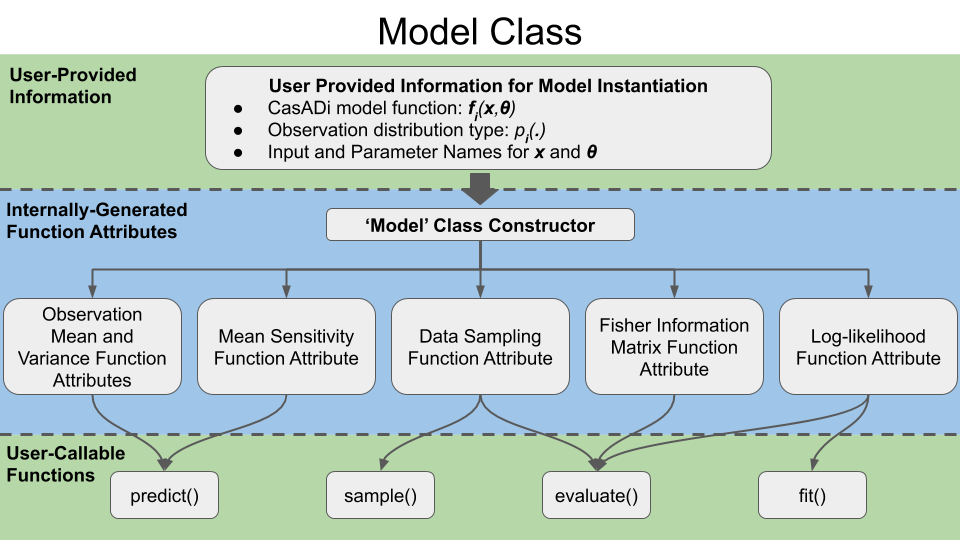
\includegraphics[scale=.4]{Images/ModelClass.png}
\caption{A diagram depicting the user-provided arguments, internal function attributes and user-callable functions of the NLOED \texttt{Model} class.}
\label{fig:model_class}
\end{figure}
At the top of the figure, the green section labeled \textit{User-Provided Information} illustrates the data a user needs to prepare in order to create an NLOED model. The required information includes the deterministic parts of the model $\bm{f}_i(\bm{x},\bm{\theta})$, encoded in a CasADi functions. It also includes the assumed observation distributions, $p_i(.)$ for each observation variable, as well as names for the model inputs and parameters. The user provides this information to the \texttt{Model} class constructor which creates the class instance. 

Instantiation is normally done in a single line of code and occurs almost instantaneously; however it hides several automated processes that generate internal \textit{function attributes} inside the class instance. These automatic processes are labelled as \textit{Internally-Generated Function Attributes} in Figure \ref{fig:model_class} and are shown in the blue region in the middle of the figure. During instantiation, the \texttt{Model} class uses the CasADi function, $\bm{f}_i(\bm{x},\bm{\theta})$, passed by the user, to auto-generate a variety of CasADi function attributes. These function attributes include atomic functions to compute the mean and variance of observations variables, the log-likelihood, the parametric sensitivities, the FIM and simulated data. These expressions are first generated symbolically and then encapsulated in a callable CasADi function stored within the \texttt{Model} class instance. The user will rarely interact with them directly, however they are used internally in many scenarios. These scenarios include when the \texttt{Model} instance is passed to the \texttt{Design} class for optimization or when the user invokes user-callable functions (discussed below) that use these auto-generated function attributes within their implementation.%Each function performs an elemental mathematical operation need for .
%These function attributes are generated quickly and silently in the background when the NLOED model is created. 

%After instantiation, the \texttt{Model} instance stores all of these new function attributes, attached to the model instance. 
The final section in Figure \ref{fig:model_class} is labelled \textit{User-Callable Functions} and it highlights various high-level functions the user can call directly to perform specific tasks using the model. For example the user can ask for predictions from the model using the \texttt{predict()} function, or the user can use the \texttt{fit()} function to fit the model parameters to a provided dataset. These high-level user-callable functions are designed to provide a simple means to perform common tasks efficiently, while hiding the more mathematical function attributes within the class. Thus the user will generally instantiate a model at the beginning of a script or session and then use that model, and its available high-level functions, to perform various computations such as designing experiments, fitting data and predicting new behaviour. In the following three subsections we go into more detail on 1) how to create a model, 2) the exact role of the auto-generated function attributes, and 3) explaining the usage of the high-level user-callable functions for fitting, predicting, sampling and evaluating designs.

\subsection{Creating a \texttt{Model} Object}

To create a \texttt{Model} class instance, the user first needs to encode the deterministic part of their model in CasADi symbolics. Recall, the deterministic part of the model are the mathematical relations, $\bm{f}_i(\bm{x},\bm{\theta})$, mapping the inputs, $\bm{x}$, and parameters, $\bm{\theta}$, to the sampling statistics, $\bm{\eta}_i$, of the observation variable, $Y_i$. Listing \ref{lst:casadi_symbols} demonstrates this process for a simple two-input, two-output, four-parameter model: \ref{eq:linear_model},
\begin{align}
\begin{aligned}
&\mu_{Y_1} = \theta_0 + \theta_1 x_1 + \theta_3 x_1 x_2,~~
\sigma^2_{Y_1} = 0.1,
&& Y_1 \sim \text{Normal}(\mu_{Y_1},\sigma^2_{Y_1}),\\
&\lambda_{Y_2} = \exp(\theta_0 + \theta_2 x_2 + \theta_3 x_1 x_2),
&& Y_2 \sim \text{Poisson}(\lambda_{Y_2}).
\end{aligned}
\label{eq:linear_model}
\end{align}
This model has a simple linear regression model for $Y_1$ and a Poisson regression model for $Y_2$.
To begin implementing this model in CasADi symbolics the \texttt{Model} class is imported from the NLOED package on line 1 of Listing \ref{lst:casadi_symbols}.
\begin{listing}[h!]
\begin{minted}[xleftmargin=\parindent,linenos,breaklines]{python}
from nloed import Model
#create casadi symbols for the inputs
x = cs.SX.sym('x',2)
#create casadi symbols for the parameters
theta = cs.SX.sym('theta',4)
#define y1 sampling statistics; mean and variance
mean_y1 = theta[0] + theta[1]*x[0] + theta[3]*x[0]*x[1] 
var_y1 = 0.1
#define y2 sampling statistics; mean and variance
rate_y2 = cs.exp(theta[0] + theta[2]*x[1] + theta[3]*x[0]*x[1])
#create a casadi function for y1 stats
eta_y1 = cs.vertcat(mean_y1, var_y1)
func_y1 = cs.Function('y1',[x,theta],[eta_y1])
#create a casadi function for y2 stats
eta_y2 = rate_y2
func_y2 = cs.Function('y2',[x,theta],[eta_y2])
\end{minted}
\caption{An example encoding a mathematical model in CasADi symbolics and creating a CasADi function, prior to instantiating a \texttt{Model} instance.}
\label{lst:casadi_symbols}
\end{listing}
Lines 3 and 5 declare CasADi symbols for the input vector, $\bm{x}$, as variable \texttt{x} and the parameter vector, $\bm{\theta}$, as variable \texttt{theta}. In lines 7 and 8 the mean, $\mu_{Y_1}$, and variance, $\sigma^2_{Y_1}$, of observation variable, $Y_1$, are defined in terms of the inputs and parameters as \texttt{mean\_y1} and \texttt{var\_y1}. In line 10 the Poisson rate, $\lambda_{Y_2}$, for observation variable, $Y_2$, is likewise defined. In line 12, the sampling statistics vector, $\bm{\eta}_1$, for observation $Y_1$ is defined as \texttt{eta\_y1}. In line 13 a CasADi function, \texttt{func\_y1}, mapping inputs and parameters to the sampling statistics for $Y_1$ is created; this CasADi function implements $\bm{f}_1(\bm{x},\bm{\theta})$. Likewise in line 15, the sampling statistic, $\bm{\eta}_2$, for observation variable $Y_2$ is defined as \texttt{eta\_y2} and in line 16 a CasADi function \texttt{func\_y2} corresponding to model function $\bm{f}_2(\bm{x},\bm{\theta})$ is also created. From the perspective of NLOED, the CasADi functions implementing $\bm{f}_i(\bm{x},\bm{\theta})$ are a computational black box and the user can use a wide range of CasADi modelling methods and different building blocks to construct these functions. Regardless of how they are built up, NLOED will auto-generate any required functionality internally. While this regression model is quite straightforward, symbolic construction can become more nuanced for dynamic models which is covered in the example section \ref{package_examples}. %Further casadi modelling examples can be found at (casadi github).

Having constructed the deterministic parts of the model as CasADi functions the user can now instantiate a \texttt{Model} object. The general call structure for the \texttt{Model} class constructor is;
\mint{python}|Model(observ_list, input_names, param_names, options={})|
\noindent The first argument, \texttt{observ\_list}, is a list of tuples, each tuple corresponds to an independent observation variable. The first entry in each tuple is the CasADi function for the sampling statistics (i.e. $\bm{\eta}_i=\bm{f}_i(\bm{x},\bm{\theta})$), the second entry is the name of the distribution assigned to that observation (i.e the type for $p_i(.)$, see Listing \ref{lst:model_constrct}). The list of observation tuples in \texttt{observ\_list} can be extended to accommodate dozens of observation variables, which becomes important for dynamic models with multiple states and time points. The second and third arguments to the \texttt{Model} constructor, \texttt{param\_names} and \texttt{input\_names}, are an input name list and parameter name list. These are both lists of strings, naming the parameters and inputs according to the order they are given to the CasADi function. Input and parameter names are required in NLOED so that any returned dataframes or graphics will be labelled intelligibly. Note that the names for the observation variables, $Y_i$, are inherited from their corresponding CasADi function strings, assigned as the first argument when the functions are created. In Listing \ref{lst:casadi_symbols} the names \texttt{y1} and \texttt{y2} were assigned in the creation of the CasADi functions \texttt{func\_y1} and \texttt{func\_y2} respectively. These names will be passed into the \texttt{Model} constructor via the CasADi functions when they are added to the \texttt{observ\_list} argument. 
\begin{listing}[h!]
\begin{minted}[xleftmargin=\parindent,linenos,breaklines,firstnumber=17]{python}
#create observation list
observ_list = [(func_y1,'Normal'),(func_y2,'Poisson')]
#creat input name list
input_names = ['x1','x2']
#create parameter name list
parameter_names = ['Theta0','Theta1','Theta2','Theta3']
#create NLOED Model
model_object = Model(observ_list, input_names, parameter_names)
\end{minted}
\caption{An example showing creation of a \texttt{Model} instance in NLOED.}
\label{lst:model_constrct}
\end{listing}
Listing \ref{lst:model_constrct} demonstrate the creation of the required \texttt{Model} constructor arguments and the calling of the \texttt{Model} class constructor. In line 18, an observation list, \texttt{observ\_list}, is constructed with a tuple for each observation variable: $y_1$ and $y_2$. The first element of each tuple is a CasADi function: \texttt{func\_y1} and \texttt{func\_y2}. The second element of each tuple is the assigned distribution; here we pass \texttt{Normal} assigning the normal distribution to $Y_1$, and \texttt{Poisson} assigning the Poisson distribution to $Y_2$. The other distribution options include; \texttt{Lognormal}, \texttt{Bernoulli}, \texttt{Binomial}, \texttt{Exponential}, and  \texttt{Gamma}. In lines 20 and 22, names are given in lists for the inputs and parameters. In line 24 the \texttt{Model} object is created with a call to the \texttt{Model} class constructor.

% Code listing \ref{lst:multiout_model_exmp} demonstrates building a model with two observations, each with a different sampling distribution. In this example we assume the experimenter has access to both mRNA and GFP measurements and that GFP is proportional to mRNA levels. It is assumed that mRNA has a lognormal distribution and that GFP is approximately normally distributed. Further we assume a quadratic model for the variance statistic, in that the variance staistics of both distributions are proportional to the square of the mean. In lines 7 and 8 we define the symbolic expressions for the mRNA sampling statistics, which are the log-mean and log-variance (more def??). Similar steps for the GFP measurments are given in lines 10 and 11. Lines 13 and 15 define the respective CasADi functions for each output and in line 20 they are both passed to the \texttt{Model} constructor with respective labels indicating the distribution they correspond to. 

% \begin{listing}[]
% \begin{minted}[xleftmargin=\parindent,linenos,breaklines]{python}
% import casadi as cs
% from nloed import Model
% #create casadi symbols for the inputs and parameters
% x = cs.SX.sym('x',1) parameters
% p = cs.SX.sym('p',6)
% #define the deterministic expression for mrna log mean and variance
% mrna_logmean = cs.exp(p[0]) + cs.exp(p[1])*x[0]**cs.exp(p[2])/(cs.exp(p[3])**cs.exp(p[2])+x[0]**cs.exp(p[2]))
% mrna_logvar = cs.exp(p[5])*mrna_mean**2
% #define the deterministic expression for GFP mean and variance
% gfp_mean = cs.exp(p[4])*mrna_mean
% gfp_var = cs.exp(p[5])*gfp_mean**2
% #create a casadi function for mrna lognormal statistics
% mrna_stats = cs.Function('mRNA',[x,p],[cs.vertcat(mrna_logmean, mrna_logvar)])
% #create a casadi function for GFP normal statistics
% gfp_stats = cs.Function('GFP',[x,p],[cs.vertcat(gfp_mean, gfp_var)])
% #define input and parameter names
% xnames = ['Inducer']
% pnames = ['Basal','Rate','Hill','HalfConst','GFPScale','VarScale']
% #define observation list
% obs_list = [(mrna_stats,'Lognormal'),(gfp_stats,'Normal')]
% #instantiate nloed model class
% model_object = Model(obs_list,xnames,pnames)
% \end{minted}
% \caption{Example encoding a multi-ouput mathematical model in CasADi symbolics and creating CasADi functions, followed by instantiating a multi-output \texttt{Model} instance.}
% \label{lst:multiout_model_exmp}
% \end{listing}



\subsection{Function Attributes of the \texttt{Model} Class}

After instantiating the model, several automatic process occur to create the previously mentioned \textit{function attributes}. The CasADi functions the user passes in the \texttt{observ\_list} argument implement the deterministic model components (i.e. $\bm{f}_i(\bm{x},\bm{\theta})$). Having the deterministic model component expressed as a CasADi function provides a powerful tool for auto-generating new mathematical expressions because CasADi functions have a dual nature as both symbolic and numeric functions. If we pass numerical values to the CasADi function, it will compute a numerical output. On the other hand, if we pass CasADi symbols to a CasADi function, the returned object is a symbolic expression. This means we can use CasADi functions to generate new symbolic expression. The expressions can then be algebraically combined as well as differentiated (via AD) to compute other new quantities symbolically. Any newly generated symbolic expressions can also be encapsulated in a CasADi function so that they can be used to generate numerical results when required. CasADi functions therefore allow this interleaving of symbolic expression building and numeric function generation which is ideal for constructing the mathematical infrastructure needed by the \texttt{Model} class. During instantiation of a \texttt{Model} object, this process is used to auto-generate and store mathematical function attributes used for experimental design, fitting and other higher-level tasks. These function attributes are available to the user but are not intended to be called directly. However they may be of use if the user wishes to perform certain model analyses that are not available as a higher-level user-callable function.
%Instead the autogenerated function attributes are used within in easier to use user-callable functions detailed later in the code. The autogenerate function attributes are also used internally within the \texttt{Design} class for structuring the design optimization problem. 
Below we give a brief overview of the auto-generated function attributes to give context for the package architecture and its internal capabilities. Note, there is a function attribute for each observation variable, $Y_i$, and the class fields where they are stored are therefore lists, indexed by the observation variable order. That is to say each field discussed below is a list of functions indexed by \texttt{[i]}, one function for each observation variable.

% \begin{itemize}
% \item \textbf{Model sampling and predictions}
%The user often needs to plot predictions from the model and understand the expected behaviour of the modeled system in a variety of scenarios after callibration.
\begin{itemize}
%\paragraph{Sampling statistics} 
\item \textbf{Sampling statistics} The CasADi functions passed by the user, implements $\bm{\eta}_i = \bm{f}_i(\bm{x},\bm{\theta})$
from the model definition. The original CasADi functions are therefore useful for predicting sampling statistics of each observation variable, conditional on the specified input and parameter values. The user provided CasADi functions are therefore stored as function attributes, one for each observation variable, in the \texttt{model[i](inputs,parameters)} field for use in other function attributes and user-callable functions. 
%\paragraph{Observation Mean and Variance} 
\item \textbf{Observation Mean and Variance }Given the conditional sampling statistics, $\bm{\eta}_i$, of each observation variable, it is also possible to compute the observations, $Y_i$'s, expected mean, $E[Y_i]$ and variance, $\textit{Var}[Y_i]$, algebraically from $\bm{\eta}_i$ at any given input and parameter value. (Note, the mean and variance are not the same as the sampling statistics for some non-normal distributions). Function attributes to compute the observation mean and variance for each observation variable, given an input and parameter vector, are auto-generated and stored in the \texttt{model\_mean[i](inputs,parameters)} and \texttt{model\_variance[i](inputs,parameters)} fields. 
%\paragraph{Mean Sensitivity} 
\item \textbf{Mean Sensitivity} Sensitivity functions for the mean observational responses, $E[Y_i]$, of each observation variable with respect to the parameters are also auto-generated. To do so we make use of CasADi's AD functionality via the \texttt{jacobian} function. The resulting function attributes returns a parametric sensitivity vector; the functions attributes are stored in the \texttt{model\_sensitivity[i](inputs,parameters)} field. 
%\item \textbf{Sampling data} Sampling data from the model is useful both for simulation studies and for Monte Carlo evaluations of different experimental designs. 
%\paragraph{Observation Sampling}
\item \textbf{Observation Sampling} Observations generated by the model are assumed to come from the conditional distribution $p_i(y_i|\bm{f}_i(\bm{x},\bm{\theta}))$. Sampling from this distribution requires the user-passed CasADi function, (i.e $\bm{f}_i(\bm{x},\bm{\theta})$), and the distributional information, (i.e. the type of $p_i(.)$). Given this information, the package can combine the correct distribution-specific random number generation from SciPy or Numpy and the \texttt{model[i](inputs,parameters)} function attributes to create a data sampling function attribute for each observation variable. These function attributes are stored in the  \texttt{observation\_sampler[i](inputs,parameters)} field. Each of these function attribute generates a single realization, $y_i$, of the given random observation variable, $Y_i$, conditioned on the input and parameter values passed.
%\item \textbf{Log-likelihood} 
%\paragraph{Log-likelihood} 
\item \textbf{Log-likelihood} The log-likelihood is needed for performing maximum likelihood fitting and is also useful in calibration diagnostics like profile likelihood intervals and traces (see the \texttt{fit()} function later in this section). The log-likelihood for an individual observation is defined as in Chapter \ref{background_chapter}, with the indices indicated there, such that
\begin{align}
l_i(y_i|\bm{x},\bm{\theta}) = \log \left[ p_i(y_i|\bm{\eta}_i{=}\bm{f}_i(\bm{x},\bm{\theta}))\right].
\end{align}
Using the type of distribution for $p_i(.)$ and the user passed CasADi function for $\bm{f}_i(\bm{x},\bm{\theta})$, the NLOED package will auto-generate a function for computing the log-probability of observing a specific observation value, $y_i$, given specified input and parameter values. The log-likelihood function attribute is stored in the class field named \texttt{loglik[i](observation,inputs,parameters)}, with one function for each observation variable.
%\item \textbf{Sensitivity and Fisher information} %Sensitivity of the model observables to the parameters often provides useful information in regarding system behaviour. In addition to sensitivity analysis for its own sake, parameteric sensitivities are also useful for propogating parameter uncertainty to prediction uncertainty via the delta method and in computing the Fisher information for experimental design. 
%\paragraph{Sensitivity and Fisher information.}
%\item \textbf{Fisher information matrix} 
%\paragraph{Fisher Information Matrix} 
\item \textbf{Fisher Information Matrix} The Fisher information matrix is a key entity used in experimental design. In evaluating a new design, each potential input-observation pair contributes an individual Fisher information matrix to the overall sum for the experiment, see Chapter \ref{background_chapter} for a full description. The Fisher information matrix for an individual input-observation pair is defined as
\begin{align}
I_i(\bm{x},\bm{\theta}) =  E_{y_i} [\nabla_{\bm{\theta}} l_i(\bm{\theta};y_i,\bm{x}) \cdot \nabla_{\bm{\theta}} l_i(\bm{\theta};y_i,\bm{x})^T ].
\label{eq:solo_fim_repeat}
\end{align}
The individual matrices, $I_i(\bm{x},\bm{\theta})$, are additive over input-observation pairs due to NLOED's assumption that all observations are independent. 
However NLOED uses the chain rule decomposition, discussed in Chapter \ref{background_chapter}, to separate the FIM computation into a sensitivity vector and a distribution-specific elemental matrix such that
\begin{align}
I_i(\bm{x},\bm{\theta}) = \nabla_{\bm{\theta}} \bm{f}_i(\bm{x},\bm{\theta}) ~\Psi(\bm{\eta}_i{=}\bm{f}_i(\bm{x},\bm{\theta})) ~\nabla_{\bm{\theta}} \bm{f}_i(\bm{x},\bm{\theta})^T.
\label{eq:element_fim_repeat}
\end{align}
Here $\nabla_{\bm{\theta}} \bm{f}_i(\bm{x},\bm{\theta})$ is the parametric sensitivity of the sampling statistics $\bm{\eta}_i$. The sensitivity vector can be computed using 
CasADi's automatic differentiation functionality applied to the user-passed model functions, $\bm{f}_i(\bm{x},\bm{\theta})$.
The elemental matrix, $\Psi(\bm{\eta}_i{=}\bm{f}_i(\bm{x},\bm{\theta}))$, is specific to each distribution \cite{fedorov2013optimal}, and can be computed algebraically from the sampling statistics, $\bm{\eta}_i$. Using this property the package is able to auto-generate a function that can compute the individual Fisher information for a given input-observation pair at a candidate parameter vector instance. 
%This function can be applied to each of inputs-observation pairs in a design and the resulting information matrices can then be summed to evaluate the experiments utility.
The FIM functions are stored in the \texttt{fisher\_info\_matrix[i](inputs,parameters)} field. These functions, like the other function attributes, are a CasADi functions and are therefore capable of both numeric and symbolic computation. The \texttt{Model} class uses this dual functionality both to compute evaluation metrics for candidate designs numerically and to construct symbolic expressions for the optimization problem solved in the \texttt{Design} class.
\end{itemize}

% Autogenerated math stuff, follows directly from casadi model function, is fast to generate on instantiation
% \begin{itemize}
%   \item Model function
%   \item Data Sampler
%   \item Log-likelihood
%   \item Sensitvitiy
%   \item FIM
% \end{itemize}

\subsection{User-callable \texttt{Model} Functions}

After instantiating a \texttt{Model} instance, the user will often follow the basic workflow outlined in Figure \ref{fig:workflow} and pass the model object into the \texttt{Design} class constructor to begin optimizing designs for the given system. However, the \texttt{Model} class provides a number of high-level user-callable functions that provide additional model building, calibration and diagnostic tools. Descriptions and usage examples for these functions are outlined below.

\paragraph{The \texttt{evaluate()} function} The NLOED package exists to optimize experimental designs for various models and objectives. In many workflows, it is reasonable to assume the user may wish to evaluate the performance of many designs for a given model using some common quantitative metrics. While the \texttt{Design} class can return the objective for its optimal (relaxed) design, this objective is generally scaled for numerical convenience and is a single number (i.e. the determinant) computed from the total Fisher information matrix. Thus the objective alone may not be interpretable or useful for intuitive comparison.
%also the user may not wish to optimize simply to get an evaluation metric, and the relaxed design's objective is only approximately related to the performance of any rounded design generated from the relaxed one.
In addition, the user may often wish to evaluate non-optimized designs implemented in existing datasets or prospective designs created using domain-specific knowledge rather than optimization. Motivated by these considerations, the \texttt{evaluate()} function accepts any candidate design (optimized or user-created) and can return interpretable comparison metrics for evaluating and comparing design performance. 

The \texttt{evaluate()} function specifically focuses on comparing designs on their prospective parameter calibration accuracy. NLOED generally assumes that all models are identifiable. Under this assumption, the \texttt{evaluate()} function gives approximate metrics about the estimate's distribution, given a design $\mathcal{D}$. 
%BPI:cite background or any ref needed therin, NEEDS a REWRITE
%The design influences $\hat{\bm{\theta}}$'s distribution by mediating the sensitivity of the estimate to sampling variability; an optimized design with a large sample size will desensitize the the estimate to the sampling error, concentrating the estimate's distribution near the true value. 
Metrics provided by \texttt{evaluate()} include the estimate's MSE, covariance and bias as well as the FIM (as discussed in Chapter \ref{background_chapter}).
Unfortunately it is impossible to compute these first three quantities exactly. However, these metrics can be approximated, either asymptotically or through simulation at a candidate point for the true parameter vector (i.e. a guess or estimate). The \texttt{evaluate()} function provides both asymptotic and Monte Carlo methods for computing these metrics for a given design. (Note, these approximations are always local and thus conditional on a nominal parameter estimate, as the true value is never actually known.) First-order asymptotic approximations for the covariance can be be computed as the inverse of the Fisher information matrix \cite{fedorov2013optimal}. As the asymptotic bias is zero at first order, the diagonal of the inverse of the FIM is an asymptotic approximation for the MSE as well (see discussion in Chapter \ref{background_chapter} for details) \cite{rilstone1996second}. The \texttt{Design} class performs all optimization using objectives based on the FIM, thus the asymptotic metrics generated by \texttt{evaluate()} are computed with similar assumptions to those used in the optimization. These methods are rapid and computationally efficient, especially with CasADi's AD tools, however they compromise on accuracy at smaller sample sizes.

Without using higher order methods, which are significantly more complicated \cite{rilstone1996second}, approximating the bias generally requires simulation-based approximations via Monte Carlo methods. The \texttt{evalutate()} method therefore also implements a parametric Monte Carlo algorithm for approximating the MSE, covariance and bias terms. The Monte Carlo method may yield greater precision than the asymptotic approach, especially at smaller sample size or with highly nonlinear models. In this method, a `true' nominal parameter vector is used to simulate a large number of datasets corresponding to the candidate design. These datasets are then each fit independently using maximum likelihood. The resulting set of estimated parameter vectors are then used to compute the MSE, covariance and bias empirically, using the nominal parameter vector as a stand-in for the unknown true values. This then provides a local approximation for the parameter accuracy metrics for the given design, conditional on the assumed true vector values. The Monte Carlo approximation is time consuming and the sample number used may need to be tuned to the design and model being evaluated in order to achieve stable approximations, as the algorithm is necessarily non-deterministic. These considerations make the Monte Carlo approach unsuitable for use in the \texttt{Design} class optimization, however Monte Carlo metrics can provide useful benchmarks to assess the suitability of asymptotically derived designs at small sample size. The Monte Carlo metrics are also valuable for comparing amongst several design candidates, allowing the user to accurately differentiate between subtle trade-offs in bias and variance components of parameter error. 

All design evaluation methods implemented in \texttt{evaluate()} are data-free, meaning they can be used to evaluate a design regardless of whether real data has been collected. This is because all of the metrics discussed here are computed as expectations, taken with respect to the data. Other comparison and diagnostic metric, such as profile likelihood-based methods, require real experimental observations and thus are not suitable for comparing existing datasets and prospective designs. Some data-dependent diagnostic tools, like profile-likelihoods, are implemented in the \texttt{fit()} function, described later in this section. 

\begin{figure}[htb!]
\centering
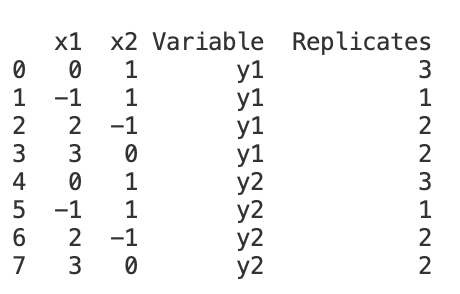
\includegraphics[scale=.7]{Images/design_examp.png}
\caption{An example of a dataframe containing an experimental design.}
\label{fig:example_design}
\end{figure}

In order to call the \texttt{evaluate()} function, the user needs to provide a design. Designs in NLOED are contained in dataframes which all follow the same format with specific naming conventions; an example of which is shown in Figure \ref{fig:example_design}. The first pair of columns each contain model input values and are named according to the input names passed by the user when the \texttt{model\_object} was instantiated. Here there are two inputs named \texttt{x1} and \texttt{x2} from the model shown in equation \ref{eq:linear_model}. To the right of the input columns is a column named \texttt{Variable} which contains the names of the observation variables to be observed at the input setting listed to the left. Here the observation variables are those from the model shown in equation \ref{eq:linear_model}; named \texttt{y1} and \texttt{y2}. The right most columns is named \texttt{Replicates} and it contains the number of observations to be taken at the given input and observation settings listed to the left. %Designs generated by NLOED will never contain duplicate rows with identical input-observation pairs. User provided designs can be passed with duplicate input-observation information in which case the replicate for the common conditions are treated cumulatively (i.e. total replicates taken at that condition are assumed to be the sum of the duplicate rows' replicate values). 

\begin{listing}[H]
\begin{minted}[xleftmargin=\parindent,linenos,breaklines]{python}
#define a design
design = pd.DataFrame({ 'x1':[0,-1,2,3]*2,
                        'x2':[1,1,-1,0]*2,
                        'Variable':['y1']*4 + ['y2']*4,
                        'Replicates':[3,1,2,2]*2})
#set nominal parameter values
param = [0.1, 2, 0.4, 1.3]
#declare specific options
eval_opts={'Method':'MonteCarlo',
           'FIM':True,
           'Covariance':True,
           'Bias':True,
           'MSE':True,
           'SampleNumber':100}
#call the evaluate() function
eval_info = model_object.evaluate(design, param, eval_opts)
#print the resulting evaluation
print(eval_info)
\end{minted}
\caption{Code example using the \texttt{evaluate()} function from the \texttt{Model} class.}
\label{lst:evaluate_call}
\end{listing}

The general call structure for the \texttt{evaluate()} function is:
\mint{python}|model_object.evaluate(designs, param, options={})|
\noindent Here the \texttt{designs} argument is a dataframe containing the candidate design to be evaluated. The \texttt{param} argument contains the nominal parameter vector at which the analysis is to take place. The \texttt{options} argument is optional and can be used to pass a dictionary of key-value pairs to alter the default \texttt{evaluate()} behaviour. An example of a call to the \texttt{evaluate()} function is shown in Listing \ref{lst:evaluate_call}. Lines 3-5 show the creation of a design dataframe and line 7 defines the nominal parameter values. In lines 9-13 various options are set in an options dictionary. The \texttt{Method} option can take two values; \texttt{Asymptotic} or \texttt{MonteCarlo} depending on which method is to be used. The \texttt{evaluate()} function by default computes metrics asymptotically, and the Fisher information matrix is always computed asymptotically. The options \texttt{FIM}, \texttt{Covariance}, \texttt{Bias}, and \texttt{MSE} accept booleans depending on whether or not the user wants the specific metric included in the returned dataframe. By default only the covariance matrix is returned. The \texttt{SampleNumber} option accepts an integer value for the samples used to generate the Monte Carlo estimates. In line 15 the \texttt{evaluate()} function is called with the previously declared arguments, and in line 17 the returned dataframe is printed.

\begin{figure}[htb!]
\centering
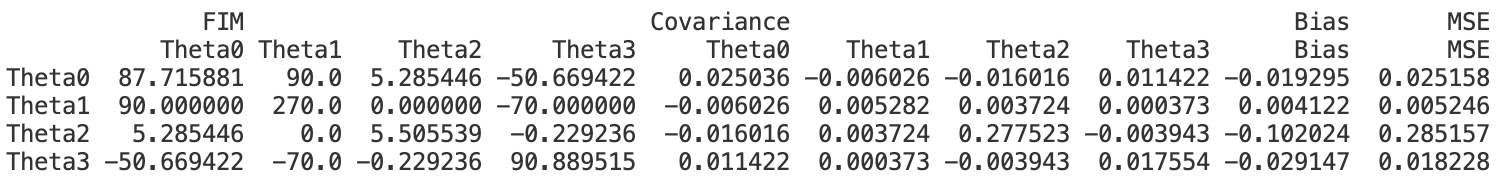
\includegraphics[scale=.56]{Images/evaluate_return.png}
\caption{An example of the dataframe returned by the \texttt{evaluate()} function, containing parameter accuracy metrics for the given design.}
\label{fig:evaluate_return}
\end{figure}

An example output for the multi-index dataframe returned by \texttt{evaluate()} is shown in Figure \ref{fig:evaluate_return}. Dataframe columns are grouped by the upper-levels \texttt{FIM}, \texttt{Covariance}, \texttt{Bias}, and \texttt{MSE}. Rows are named according to the parameter names passed by the user when the given model was instantiated. The \texttt{FIM} upper-level contains columns named for each parameter, mirroring the rows. Each entry in these columns gives the Fisher information matrix values for the model in the given experiment. The \texttt{Covariance} upper-level likewise contains columns for each parameter and gives the expected covariance matrix entries. The \texttt{Bias} upper-level contains a single column with values, in each row, for the bias of each parameter. The \texttt{MSE} level likewise contains a single column, with the expected MSE for each parameter with respect to the nominal true value in the given design.

The \texttt{evaluate()} function does not return Wald confidence intervals for the parameters. (Wald intervals are asymptotic intervals generally computed using the FIM, see \cite{seber2003nonlinear}. However, these are easily generated from the root of the diagonal of the covariance matrix, which yields the standard deviation for each parameter. Other similar metrics such as the generalized variance and alphabetic optimality criteria, can be easily computed from the returned metric (see Chapter \ref{background_chapter} for some discussion). The \texttt{evaluate()} function can also be run in a batch mode, where multiple designs are passed as a list to the \texttt{designs} argument. In this case the returned object is a list of dataframes, each structured like the previous example. The batch mode is useful for evaluating many design variants at once and automating the comparison process.
%(should add batch mode for parameters?!)

\paragraph{The \texttt{sample()} function}

%Optimal experimental design is often used in an iterative manner. The user often begins OED analysis with a candidate model and either some initial parameters estimates from the literature or some initial data used for preliminary fits. Starting from this point the package can be used to design experiments and refine model calibration in multiple rounds of optimal design, experiment, and calibration. However, between each stage of real world experimentation there is generally ample time for theoretical analysis of the model fit and the next round of experiments; an hour on the computer is generally requires less active involvement and is cheaper than an hour in the lab. 


The \texttt{sample()} function is provided in order to generate simulated data from the model.
This is useful for generating more detailed diagnostics about specific aspects of a design via simulation studies.
%Optimal designs are expected to perform well on the very specific metric they were optimized for but this performance often comes at the expense of other considerations, especially overall robustness to uncertainty. Evaluating these trade-offs is best done through simulation studies, where simulated experiments can be run comparing competing optimal designs, and their various performance trade-offs can be evaluated rigorously without as many approximations. 
Simulation studies involve simulating data for a given experimental design and performing batch fitting and evaluation on the resulting set of fits to study expected statistical properties of the fitting process.
%It is also useful in creating posterior predictive checks when large datasets are available (cite), a method developed for Bayesian models, where data is simulated from the model under prior uncertainty to qualitatively check if it looks like a real datasets in terms of its variance structure and general trend.
To this end, the \texttt{sample()} function can generate artificial datasets by sampling observations $y_i$ from the observation distribution $p_i(y_i|\bm{f}_i(\bm{x},\bm{\theta}))$ for each replicate specified in a given design, and at a given nominal parameter vector.

\begin{listing}[H]
\begin{minted}[xleftmargin=\parindent,linenos,breaklines]{python}
#define a design
design = pd.DataFrame({ 'x1':[0,-1,2,3]*2,
                        'x2':[1,1,-1,0]*2,
                        'Variable':['y1']*4 + ['y2']*4,
                        'Replicates':[3,1,2,2]*2})
#set nominal parameter values
param = [0.1, 2, 0.4, 1.3]
#call the sample() function
dataset = model_object.sample(design, param, design_replicates=1)
#print the resulting dataset
print(dataset)
\end{minted}
\caption{Example using the \texttt{sample()} function from the \texttt{Model} class.}
\label{lst:sample_func1}
\end{listing}

In order to call the \texttt{sample()} function, the user must provide a dataset in a dataframe, using the previously detailed naming convention (see Figure \ref{fig:example_design}). 
%This design can be manually created, or as is often the case, generated by the \texttt{Design} class. An example dataset was shown in figure \ref{fig:example_design}. 
The general call structure for the \texttt{sample()} function is:
\mint{python}|model_object.sample(designs, param, design_replicates=1,options={})|
\noindent The \texttt{design} argument accepts a dataframe with format depicted in Figure \ref{fig:example_design}. The \texttt{param} argument contains the nominal parameter values at which the samples are to be taken. The \texttt{design\_replicates} option is an optional argument that specifies the number of replicate datasets to generate from the design. The default value is a single dataset however when doing simulation studies it is useful to be able to generate batches of datasets for a given design and nominal parameter value. The \texttt{options} argument is optional and accepts a dictionary of key-value pairs that can modify the default behaviour of the the \texttt{sample()} function. An example call to \texttt{sample()} is shown in Listing \ref{lst:sample_func1}. In lines 2-5 an example design dataframe is created, and in line 7 nominal parameter values are listed. In line 8 the \texttt{sample()} function is called and a simulated dataset is created as a dataframe; in line 11 the returned dataframe is printed. The \texttt{sample()} function returns a dataframe containing the simulated dataset. All datasets in NLOED follow the same structure and naming convention; an example dataset is shown in Figure \ref{fig:fit_dataset}. The first pair of columns correspond to the model input settings and are named according to the string names passed during model instantiation; here they are \texttt{x1} and \texttt{x2} as per the model given in equation \ref{eq:linear_model}. Following the input columns there is the \texttt{Variable} column which contains the name of the observation variable, here \texttt{y1} and \texttt{y2} as per the model in equation \ref{eq:linear_model}. Finally, there is the \texttt{Observation} column which contains the numeric values of the observed samples.
\begin{figure}[htb!]
\centering
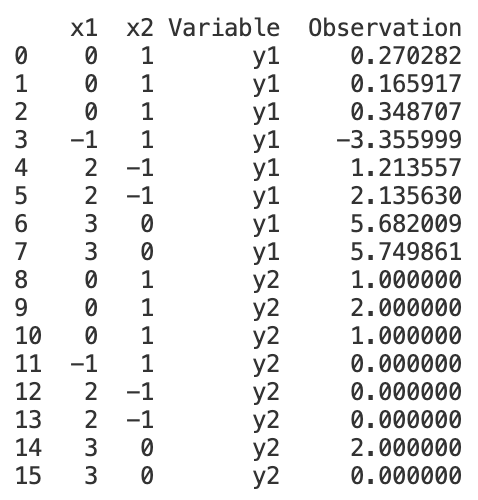
\includegraphics[scale=.7]{Images/Fit_exmp_dataset.png}
\caption{An example dataset generated from the \texttt{sample()} function.}
\label{fig:fit_dataset}
\end{figure}

The \texttt{sample()} function can also be run in a batch mode for generating datasets from multiple designs at the same time. To run a batch of designs, each design should be added to a list which is then passed in as the \texttt{designs} argument. This can be coupled with the \texttt{design\_replicates} argument to generate a specified number of replicates of each design. In batch mode the returned object is a list of dataframes for each dataset. When replicates are also included, the returned object is a list of lists, where the first dimension indexes the design and the second indexes the replicate number. 
%should provide option to have replicates sampled under a prior?? (with optional return type listing the parameter values used for each replicate?)

%fit paragraph
\paragraph{The \texttt{fit()} function} Model fitting is an important part of the workflow when generating model-based optimal experimental designs. Fitting is needed for estimating parameters from real data; data that can be preliminary or the result of optimal experiments. It is also valuable for performing simulation studies before experiments are run to give users an idea of the true expected utility of their experimental plans. All fitting functionality in the package is provided via the \texttt{fit()} function. The \texttt{fit()} function is also provided as a matter of convenience, as the type of fitting algorithm to be used for a given optimized design is not arbitrary. The \texttt{Design} class performs experimental optimization using various objectives based on the Fisher information matrix. The primary justification for using the FIM is that it provides an asymptotic estimate of the parameter uncertainty that can be achieved after fitting with maximum likelihood. The FIM and other information matrices are asymptotic for the specific model, at the guessed parameter values and \textit{for the given fitting method} \cite{fedorov2013optimal}. This means that the optimized experiment should be paired with its appropriate fitting method for the best results. Using \texttt{fit()} for fitting the user's model ensures the appropriate maximum likelihood fitting algorithm is used in all cases.

In order to fit data using the \texttt{fit()} function, the user needs to provide a dataset as an argument. Datasets passed to the \texttt{fit()} function follow the same format as other datasets in NLOED, see Figure \ref{fig:fit_dataset} for an example.
The general call structure for the \texttt{fit()} function is shown below. 
\mint{python}|model_object.fit(datasets, start_param=None, options={})|
\noindent The \texttt{datasets} arguments accept a dataframe, structured as in Figure \ref{fig:fit_dataset}. The \texttt{start\_param} argument is optional, but can be used to initialize the optimization to a specific initial parameter point. The \texttt{options} argument, is a dictionary with various key-value pairs that can be used to override specific default behaviours of the fitting algorithm, some of which are outlined below. The \texttt{fit()} function solves for the maximum likelihood estimate with a call to the nonlinear programming package IPOPT via the CasADi interface.  In order to set up the log-likelihood optimization for the IPOPT call, \texttt{fit()} uses the log-likelihood function attributes that are auto-generated in the \texttt{Model} object's instantiation. The overall likelihood objective is constructed by iterating through the rows of the passed dataset, applying the appropriate log-likelihood function attribute to each input-observation pair, and summing the result. This produces a CasADi symbol for the overall fitting objective (see Chapter \ref{background_chapter} for further discussion of maximum likelihood),
\begin{align}
l_{Tot}(\bm{\theta};\bm{y}_\mathcal{D},\mathcal{D}) = \sum_j^N \sum_i^M \sum_k^{\beta_{i,j}} l_i(y_{i,j}^{(k)};\bm{x}_j,\bm{\theta}).
\end{align}
%Here $j$ indexes the sample in the dataset, each of which has a specific observation variable index $j(i)$. 
%BPI: NEED TO MAKE CONSISTENT WITH INTRO, j(i) specifically
As the objective is a symbolic expression, when it is passed to IPOPT via the CasADi interface, any required derivative information for the interior-points algorithm is automatically generated. This ensures the maximum likelihood fitting implemented in \texttt{fit()} occurs rapidly in a few iterations for most models.

\begin{listing}[H]
\begin{minted}[xleftmargin=\parindent,linenos,breaklines]{python}
# set specific fitting options
fit_opts={'Confidence':'Intervals',
          'InitParamBounds':[(-1,1),(-1,1),(-1,1),(-1,1)],
          'InitSearchNumber':7}
#call the fit() function
fit_info = model_object.fit(dataset, options=fit_opts)
#print the fitting information
print(fit_info)
\end{minted}
\caption{Example using the \texttt{fit()} function from the \texttt{Model} class.}
\label{lst:fit_func1}
\end{listing}

A generic call to the \texttt{fit()} function is shown in Listing \ref{lst:fit_func1}, this code assumes \texttt{dataset} contains an existing dataset like the one shown in Figure \ref{fig:fit_dataset}. In lines 2-4, several options for the \texttt{fit()} function are modified. The \texttt{Confidence} option has been set from the default value of \texttt{None} to \texttt{Intervals} which signals to the fitting algorithm that it should generate profile likelihood-based confidence intervals for all fitted parameters after fitting \cite{kreutz2013profile}.
%(Likelihood-based confidence intervals are based on asymptotic properties of the log-likelihood ratio; while both likelihood-based and Wald intervals have asymptotic justifications, likelihood-based intervals require observed data where as Wald intervals do not (cite).)
The \texttt{InitParamBounds} option has been set with a list of tuples specifying a range for each parameter over which a coarse fitting pre-search is performed. The \texttt{InitSearchNumber} option specifies the number of evaluations to perform in the \texttt{InitParamBounds} ranges; here we have set it to seven but its default value is three. The pre-search procedure is performed to ensure the starting parameter vector is reasonable and the pre-search is a good recourse if a suitable \texttt{start\_param} cannot be specified \textit{a priori}. If a \texttt{start\_param} value is specified and the pre-search option \texttt{InitParamBounds} is also passed, the \texttt{start\_param} is appended to the pre-search evaluation list but it may not actually be used as the start value for IPOPT's maximum likelihood optimization as a more suitable starting value may be found during the pre-search. Note, that \texttt{InitParamBounds} are not bounds for IPOPT's optimization, only the pre-search, and that \texttt{fit()} does not allow bounded or constrained maximum likelihood fitting. The user is expected to use parameter transformations to ensure models are specified properly (examples of this are given in Section \ref{package_examples}). As maximum likelihood estimates are invariant under parameter transformation, any required re-parameterization should not effect the resulting fits \cite{pawitan2001all}. In lines 6 the \texttt{fit()} function is called for the provided dataset and in line 8 the fitting information is printed to the console.

An example output of the dataframe returned by the \texttt{fit()} function is shown in Figure \ref{fig:fit_ouput}. The returned value is a multi-index dataframe, which is organized by the upper level labels \texttt{Estimate}, \texttt{Lower}, and \texttt{Upper}. The \texttt{Estimate} level contains columns for each parameter, named according to the names passed when the model was instantiated. These columns contain the maximum likelihood estimates for the model parameters. The \texttt{Lower}, and \texttt{Upper} levels also contain columns for each parameter with the corresponding upper and lower bounds for the requested likelihood-based intervals. These columns are only returned if the \texttt{Confidence} option is set to something other than \texttt{None}, such as \texttt{Intervals} in this example. By default a 95\% confidence interval is returned.

\begin{figure}[htb!]
\centering
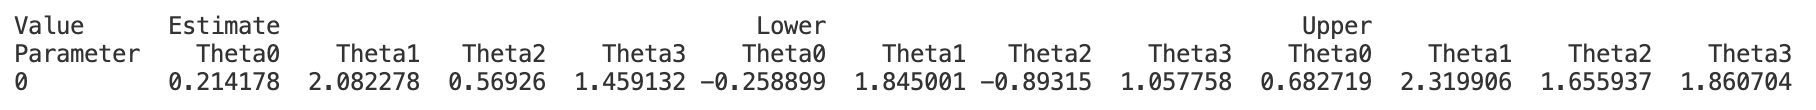
\includegraphics[scale=.48]{Images/fit_output.png}
\caption{An example of the dataframe output from a call to the \texttt{fit()} function.}
\label{fig:fit_ouput}
\end{figure}

The intervals returned via a call to the \texttt{fit()} function are computed using the profile likelihood with the observed data \cite{kreutz2013profile,pawitan2001all}. Profile likelihood confidence intervals are based on asymptotic properties of the likelihood ratio, defined as $-2L_{Tot}(\bm{\theta}_o)/L_{Tot}(\hat{\bm{\theta}})$ \cite{pawitan2001all}. Using properties of the likelihood ratio, it can be shown that  
 \begin{align}
 -2[l_{Tot}(\bm{\theta}_o)-l_{Tot}(\hat{\bm{\theta}})]\leq   \chi^2_{p,(1-\alpha)}.
 \end{align}
 Here the expression on the left of the inequality is equivalent to the likelihood ratio. The $l_{Tot}(.)$ function is the overall log-likelihood for the dataset, $\hat{\theta}$ is the MLE parameter estimate and $\theta_o$ is the unknown true parameter value. The $\chi^2_{p,(1-\alpha)}$ term is the $1-\alpha$\% percentile of a Chi-square distribution, with $p$ degrees of freedom where $p$ is the number of dimensions of $\bm{\theta}$. Effectively, the above inequality states that the likelihood ratio between the unknown true parameter vector and the MLE estimate should be less than $\chi^2_{p,(1-\alpha)}$ with a probability of $1-\alpha$\% \cite{seber2003nonlinear,bates1988nonlinear}. To construct intervals for each parameter dimension using the above result, each dimension is \textit{profiled}. Profiling each dimension allows the confidence intervals for a single dimension to properly account for uncertainty in the other parameters (see \cite{kreutz2013profile,pawitan2001all} for further discussion). Profiling a given dimension, $\theta_i$, involves incriminating its value away from the MLE value; first in an increasing direction and then a decreasing directions, although the order is arbitrary. At each increment of $\theta_i$ the other marginal parameter dimensions are re-optimized to yield a new conditional MLE for the marginal parameters given the fixed incremented value of $\theta_i$. The resulting parameter vector, including the current value of $\theta_i$ and the conditionally optimized marginal parameters, is notated $\bar{\bm{\theta}}(\theta_i)$. As the value, $\theta_i$, of the profiled dimension is adjusted away from the MLE the conditional estimate $\bar{\bm{\theta}}(\theta_i)$ traces out a curve in parameter space, this is known as the \textit{profile trace} \cite{bates1988nonlinear}. The likelihood ratio,
  \begin{align}
 -2[l_{Tot}(\bar{\bm{\theta}}(\theta_i))-l_{Tot}(\hat{\bm{\theta})}],
 \end{align}
 between the MLE, $\hat{\bm{\theta}}$, and the conditional vector, $\bar{\bm{\theta}}(\theta_i)$, will grow until it reaches the Chi-square threshold, $\chi^2_{p,(1-\alpha)}$. The values of $\theta_i$, both in the positive and negative directions, that make the Chi-squared inequality strict are considered the bounds of the the $1-\alpha$\% confidence interval for dimension $\theta_i$. The value of the log-likelihood, $l_{Tot}(\bar{\bm{\theta}}(\theta_i))$, for each value of $\theta_i$ is known as the \textit{likelihood profile} \cite{kreutz2009systems}; its maxima occurs when $\theta_i$ is at its MLE value. The profiling procedure can be performed for each parameter dimension in the parameter vector, yielding an interval, trace and profile for every dimension.
 
%  This statement can be used to construct approximate intervals by replacing the unknown true parameter, $\theta_o$, with the the variable $\theta$ and finding the values of $\theta$ that bracket the estimate, $\hat{\theta}$, and make the non-strict inequality an equality. These bracketing value of $\theta$ are the extrema in parameter space that satisfy the inequality and form the bounds on the 95\% confidence interval. The above approach can be applied with the substitution of $p$ degrees of freedom on the Chi-square distribution, and by holding all parameters but the target dimension for the confidence interval fixed at their MLE values. When dealing with multi-parameter models, the likelihood ratio statistic inequality becomes;
%  To account for this interaction effect in the multi-dimensional case, intervals can instead be computed using \textit{profile likelihoods} \cite{kreutz2013profile}. In the multi-dimensional case, the likelihood ratio statistic inequality is now;
%  Profile likelihood confidence intervals for a given profiled dimension, $\theta_i$, still involve finding extreme points that satisfy a likelihood ratio statistics inequality, however now the marginal parameters are allowed to vary from the MLE values. 
%   \begin{align}
%  -2[l_{Tot}(\bar{\bm{\theta}}(\theta_j))-l_{Tot}(\hat{\bm{\theta})}] = \chi^2_p(0.95)
%  \end{align}
%  are re-optimized to yield a new maximum likelihood estimate, $\bar{\bm{\theta}}(\theta_i)$, but with profiled dimension, $\theta_i$, held fixed at the incremented value. This sequence of conditional maximum likelihood estimates corresponds to a sequence of decreasing likelihood values, in both the positive and negative directions. The sequence of estimates constitute the \textit{log-likelihood trace} and the sequence of log-likelihood objective values corresponding to each point constitutes the \textit{log-likelihood profile}. The upper and lower bounds for $\theta_j$ are found when;
% , i.e. when the profile intersects the Chi-square bound. 
%  Likelihood profiling involves iterating over each parameter dimension, $\theta_i$, in the parameter vector estimate $\bm{\theta}$; 

When the \texttt{Intervals} value is passed as the \texttt{Confidence} option, the \texttt{fit()} function currently uses a bisection search to find the profile likelihood interval boundary points rather than completing a full incremental profile.
%BPI: DONE NEED TO REMOVE OR CLEARLY NOT AS OPTIONAL, NEWTONS ETC.
%but Newton's method and other higher-order root finding procedures are also available for certain problems via CasADi's ability to differentiate the solution of the profile likelihood optimization.
Beyond intervals, the \texttt{fit()} function can also generate other useful diagnostic information. The \texttt{Confidence} field can also be set to the value \texttt{Profiles} to generate graphical plots of the likelihood profiles and 2D projections of the profile traces for the given dataset. Examples of the profiles and trace projections are shown in \ref{fig:fit_profiles_traces}. 
\begin{figure}[htb!]
\centering
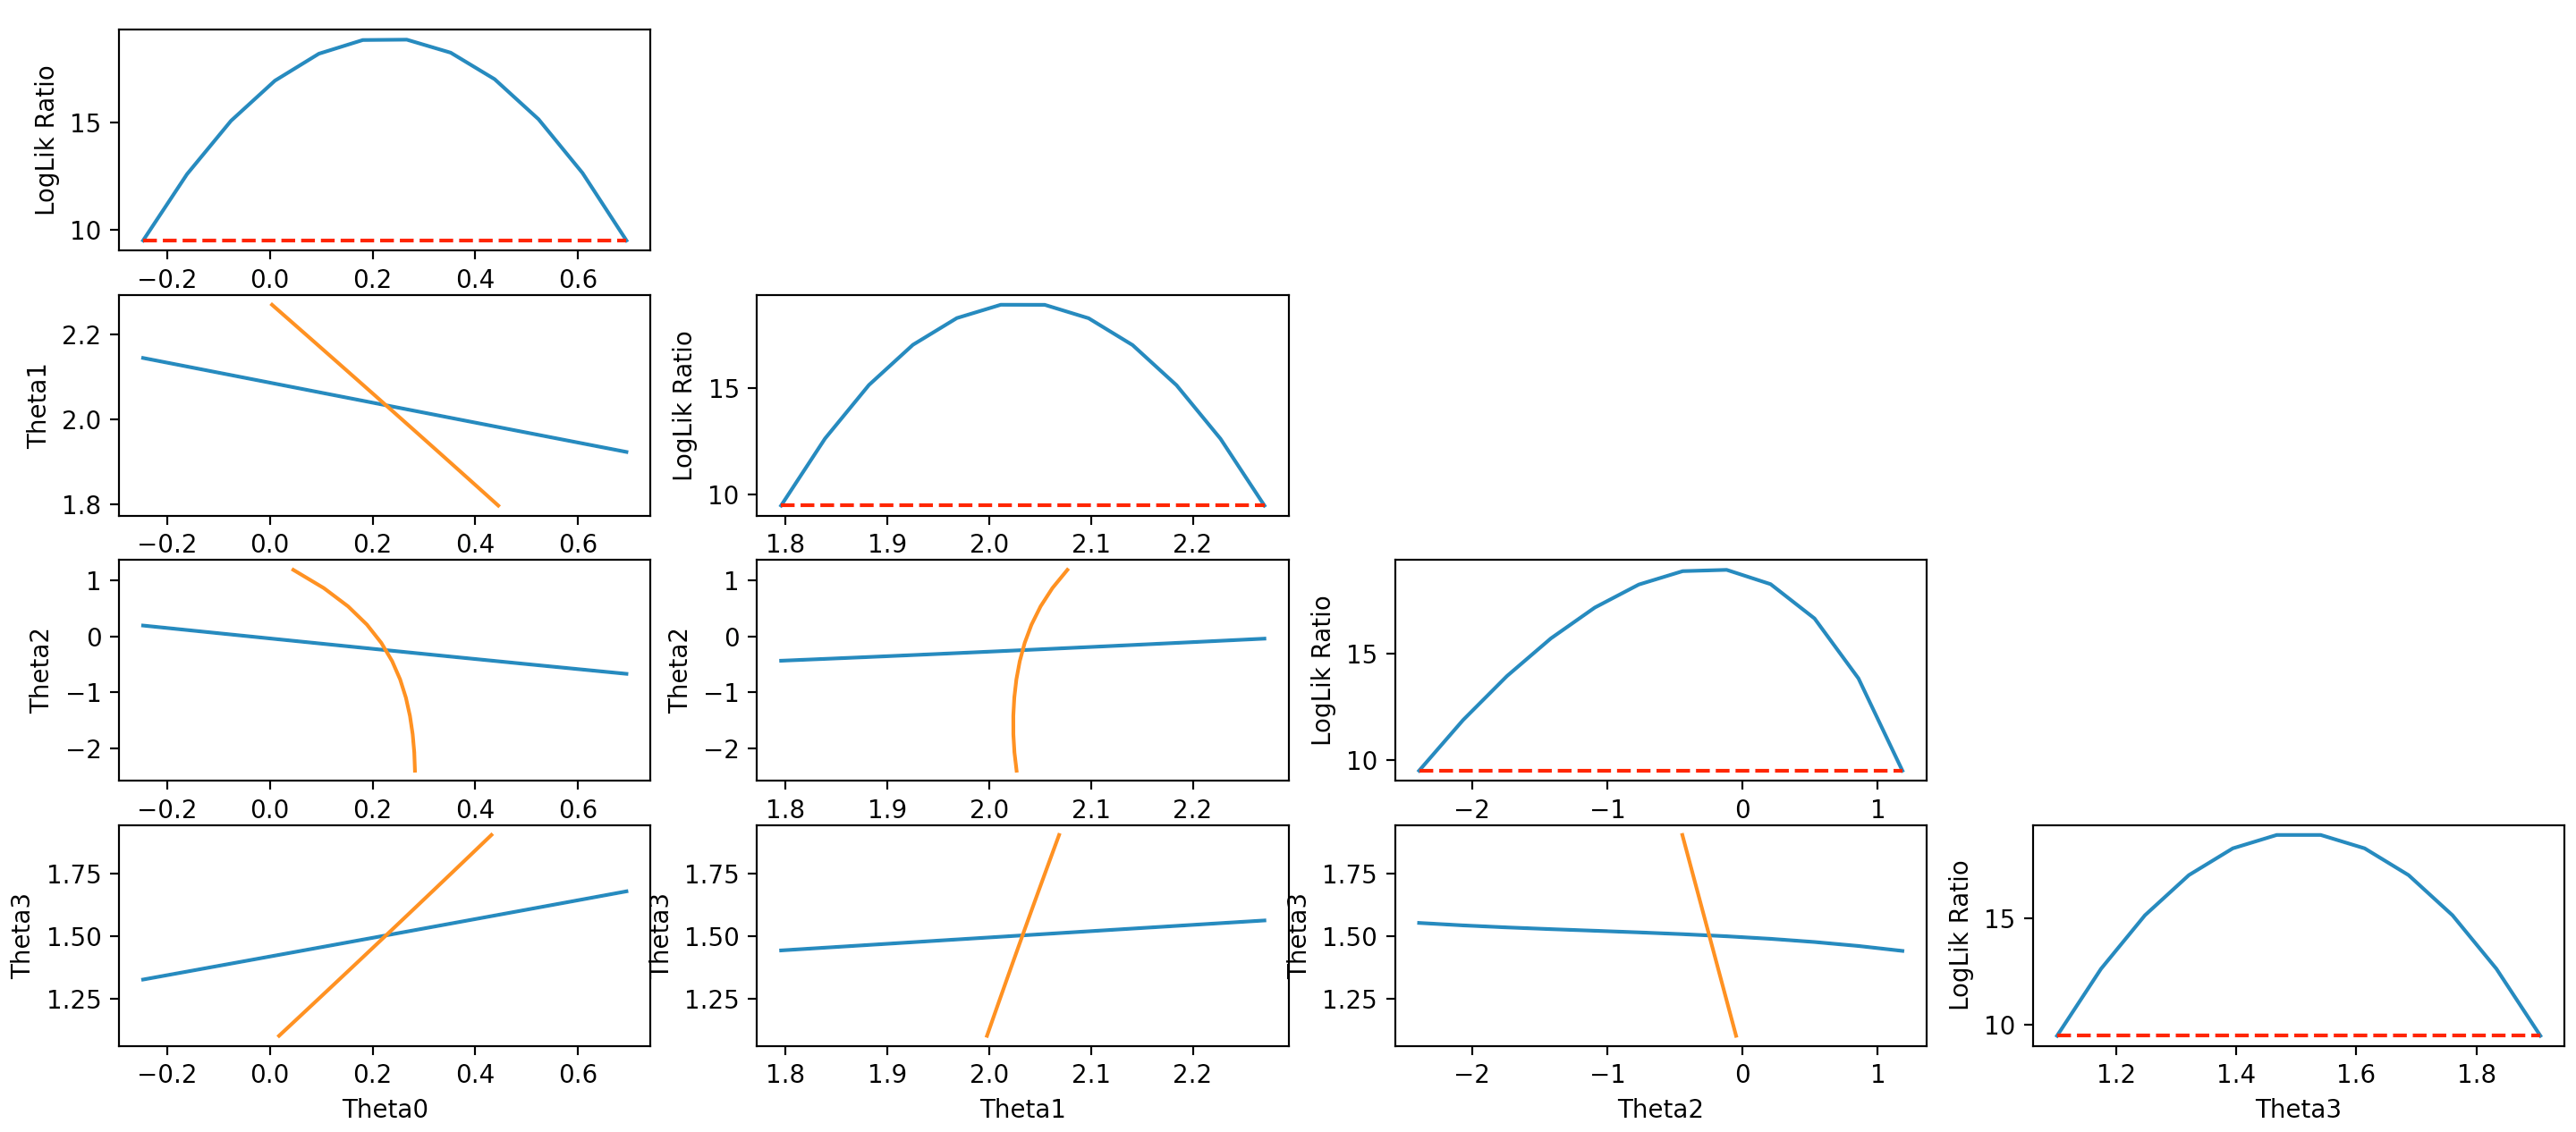
\includegraphics[scale=.33]{Images/profile_plots.png}
\caption{Example of the \texttt{fit()} functions graphical output of likelihood profiles and 2D trace projections generated when the \texttt{Confidence} option is set to \texttt{Profiles}.}
\label{fig:fit_profiles_traces}
\end{figure}
The plots on the diagonal show each parameter's profile likelihood plot, with the log-likelihood values for the profile shown on the y-axis and the the value of the profiled parameter, $\theta_i$, on the x-axis. The MLE value of the profiled parameter occurs at the profile maximum. The red dashed line indicates the log-likelihood value at which the Chi-squared threshold is reached (the default is for a 95\% interval). The intercepts between the likelihood profile and the threshold line denotes the confidence interval end points. In the lower triangular plots, a plane for each pair of the parameters is shown in which 2D projections of each parameter's profile trace are plotted as lines; the blue line belongs to parameter in the given column (profile plot above) and the orange line belongs to the parameter in the given row (profile plot to the right). The trace projections are terminated at the confidence interval boundaries, and their intersection marks the MLE estimate. Returning profiles and trace projections is useful because the shape of the log-likelihood profile, when plotted with respect to the corresponding parameter as in Figure \ref{fig:fit_profiles_traces}, should be asymptotically quadratic; significant deviations from this trend can indicate poorly identified parameters \cite{pawitan2001all}. Specifically, a blunt peak to the profile can indicate that the current data is insufficient to constraint the parameter values \cite{kreutz2009systems}. In addition, the projections of the profile traces for each parameter should be asymptotically `X' shaped, with the MLE estimate at the intersection point \cite{bates1988nonlinear}. Curvature of the trace projections as they move away from the intersection can indicate significant non-linear effects and the breakdown of the asymptotics. In addition, the profile trace projections should ideally intersect at near right angles, with highly oblique angles indicating significant correlation between parameter pairs and possible deficiencies in the experimental design.

%BPI: need to add some external cite for contour alg, its not in background anymore
 The \texttt{fit()} function can also compute likelihood \textit{contour projections} by setting the \texttt{Confidence} option to \texttt{Contours}. Likelihood contour projections consist of a closed curve surrounding the maximum likelihood estimate in a 2D projection of the parameter space \cite{bates1988nonlinear}. These curves mark the extreme points that the given pair of parameters can extend out from their MLE value before the log-likelihood ratio increases to the asymptotic Chi-square threshold, assuming the marginal parameters have been conditionally optimized (i.e. profiled) \cite{bates1988nonlinear}. The profiling algorithm used for the confidence interval computation can be modified to find likelihood contour projections in 2D parameter-pair planes by profiling along non-axial parameter vectors rather than along parameter axes. 
 %Now instead of computing $\bar{\bm{\theta}}(\theta_i)$, we instead compute \bar{\bm{\theta}}(\theta_i,\theta_j), where both $\theta_i$ $\theta_j$
 %Computing contour projections is essentially the same process as computing the boundary points of the profile likelihood intervals, except the profiling is now done with pairs of parameters along a given vector. 
 Just like the profile trace, the algorithm begins at the MLE vector, but rather than selecting an individual parameter, a pair are selected; $\theta_i$ and $\theta_j$. This pair forms a 2D plane in the parameter space. Next a grid of angles is selected from $0$ to $2\pi$ radians, each angle corresponds to a direction vector in the parameter-pair plane emanating from the MLE vector. The parameter pair, $\theta_i$ and $\theta_j$, are incremented along this vector for each angle in the grid, and the remaining marginal parameters are optimized at each point yielding a conditional MLE vector $\bar{\bm{\theta}}(\theta_i,\theta_j)$, given the fixed values of $\theta_i$ and $\theta_j$. When the a parameter pair is found along the current direction vector that satisfies the equality,
\begin{align}
-2[l_{Tot}(\bar{\bm{\theta}}(\theta_i,\theta_j))-l_{Tot}(\hat{\bm{\theta})}] = \chi^2_{p,(1-\alpha)},
\end{align}
the position in parameter space is recorded as a member of the $1-\alpha$\% profile contour projection for that parameter pair. This is repeated for each angle and parameter pair to build a set of 2D contour projections for each parameter pair. Some interpolation of the recorded contour points is used to generate smooth curves during plotting. When the \texttt{Confidence} option is set to \texttt{Contours}, contour projection plots are added to the profile and trace projection plots previously discussed. An example of the profile and trace plots with added contours is shown in Figure \ref{fig:fit_profiles_contours}.
\begin{figure}[h!]
\centering
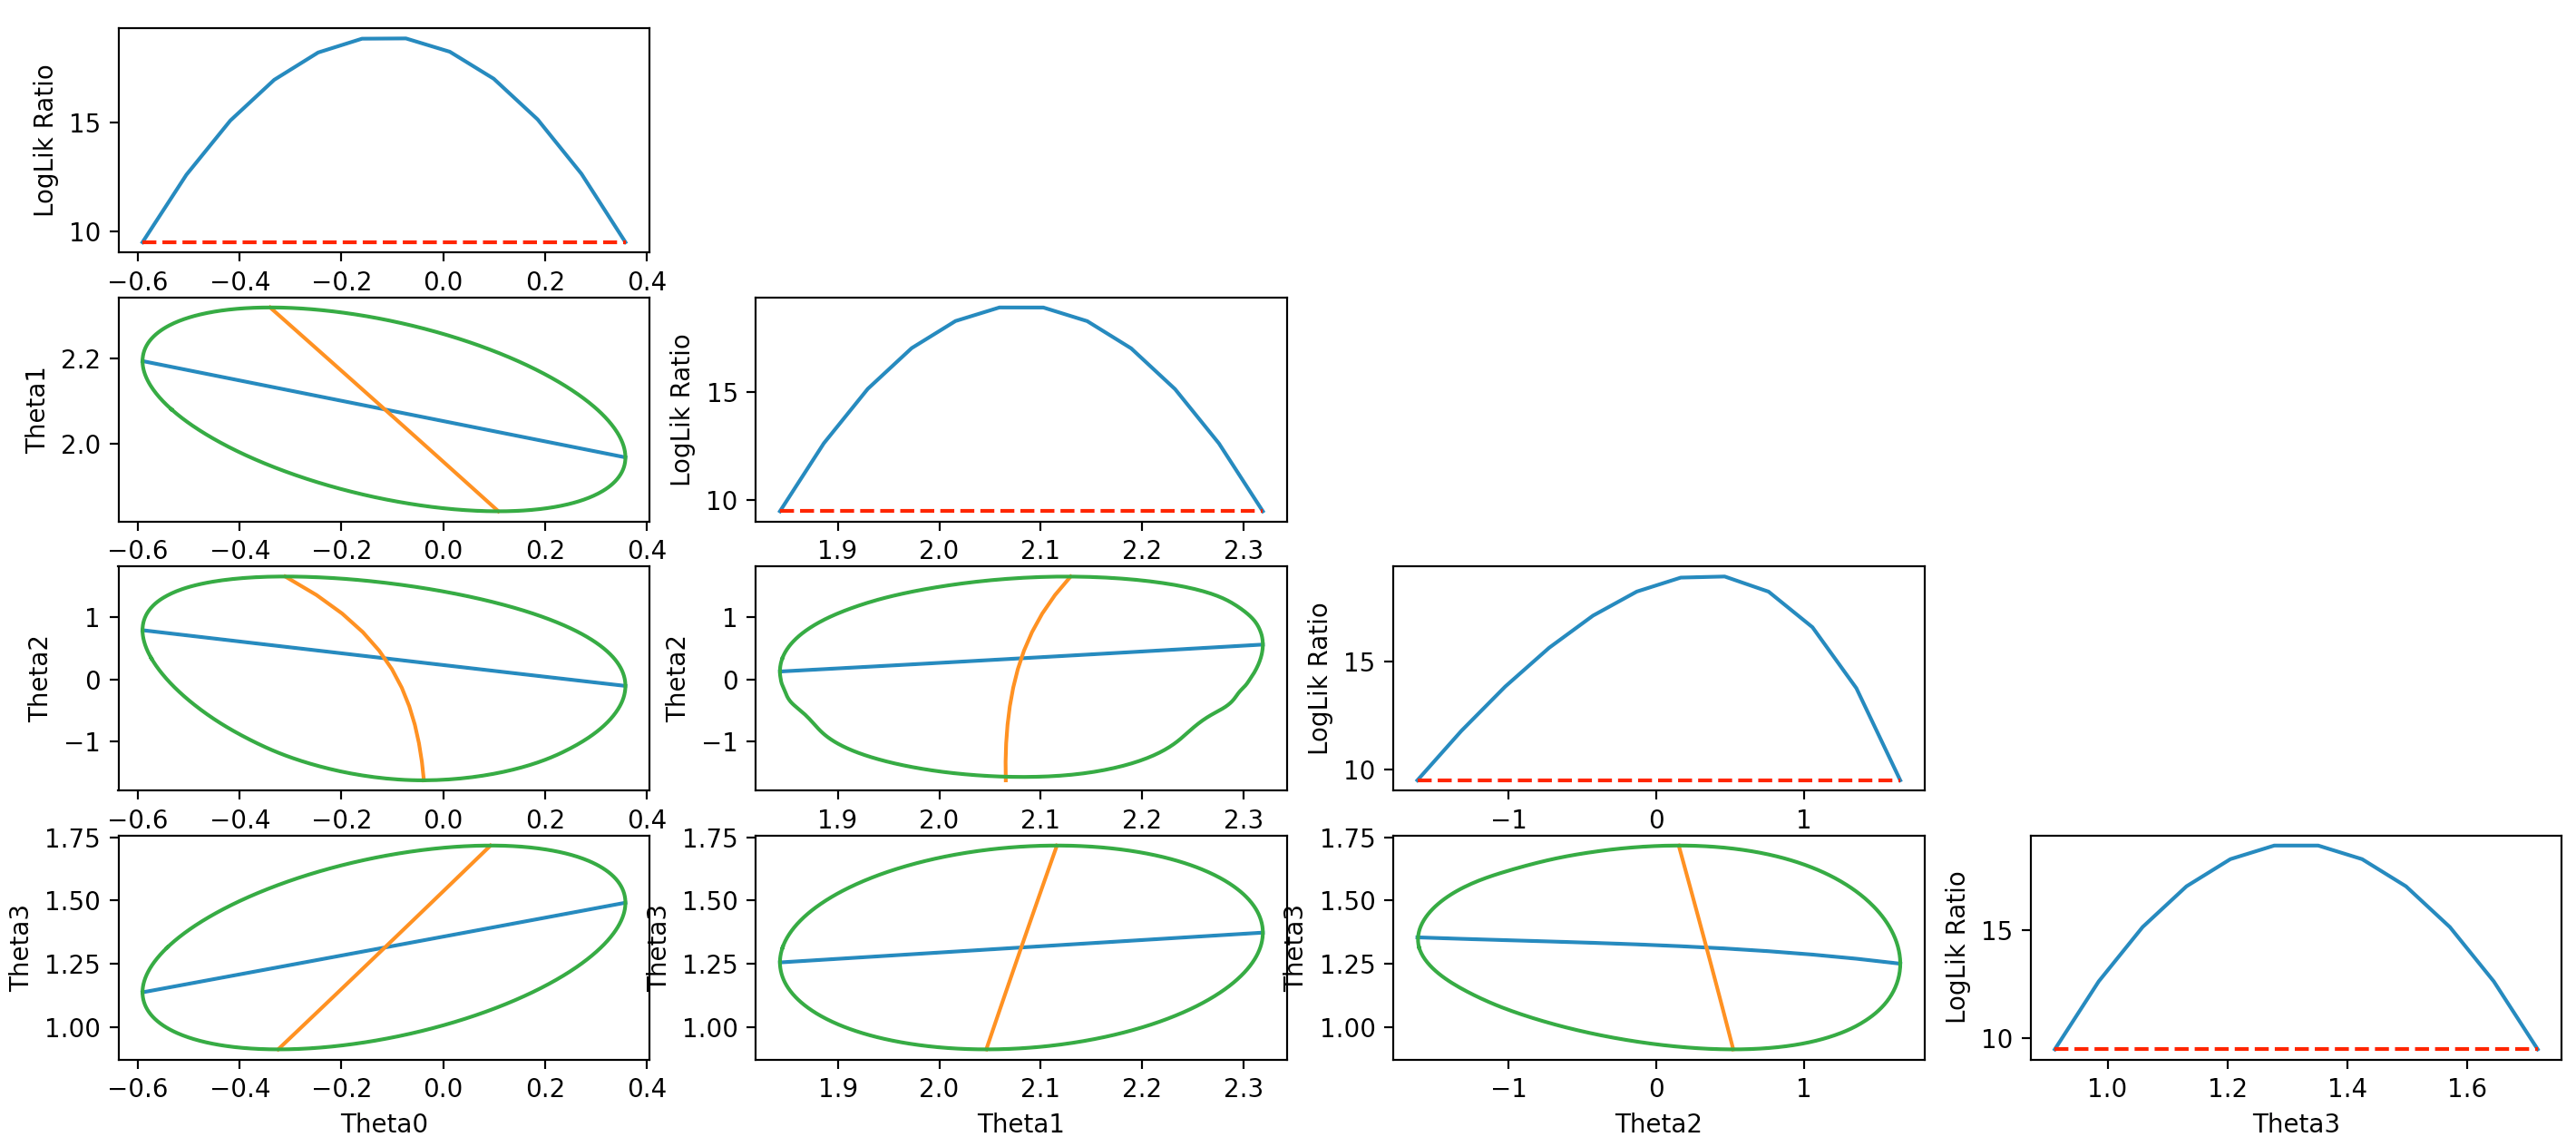
\includegraphics[scale=.31]{Images/contour_plots.png}
\caption{Example of the \texttt{fit()} function's graphical output of likelihood contour projections generated when the \texttt{Confidence} option is set to \texttt{Contours}. The contour projections are shown along with the profiles and trace projections previously shown in figure \ref{fig:fit_profiles_traces}. }
\label{fig:fit_profiles_contours}
\end{figure}
%Note the contour projections, not just slices of the confidenc cvregion occurring in the parameter pair plane fixed at the origin.
By computing contour projections for each pair of parameters, we can gain an understanding of what parameter sets are feasible given a certain confidence level. The contour projections are asymptotically ellipsoidal but model non-linearity and weak experimental designs can lead to eccentric shapes. Computing the contour projections will generally fail if the region is so eccentric that it contains large concave sections in its boundary. Computing contour projections can be time consuming, especially for large and dynamic models. Currently \texttt{fit()} uses a bisection search along each angle to find the contour points, similar to the search used for interval computation.

%For large models, the profile trace projections can be used to efficiently get a sense for the shape of the overall contour without necessarily computing them, as the trace projection endpoints always lie on the contour. 
%In such cases the ray tracing approach will intersect the boundary twice, possibly destabilizing the numerical search and leading to inaccurate boundaries. In such cases it may be possible to get an accurate boundary for a smaller percentile than the default 95\% confidence.

 %The generated plots are ordered similar to those generated when \texttt{Profiles} was requested. However, now each parameter pair plot has a contour boundary shown in green which has been interpolated from the contour points found by the algorithm. 

\begin{listing}[H]
\begin{minted}[xleftmargin=\parindent,linenos,breaklines]{python}
#create three datasets
data1, data2, data3 = dataset = model_object.sample(design, param, design_replicates=3)
#combine datasets into a single list
datasets = [data1, data2, data3]
# set up specific options for fitting
fit_opts={'Confidence':'Intervals'}
#call the fitting procedure
fit_info = model_object.fit(datasets,options=fit_opts)
#print the fitting information
print(fit_info)
\end{minted}
\caption{Example using a batch call of the \texttt{fit()} function from the \texttt{Model} class.}
\label{lst:fit_batch_fit}
\end{listing}

The intervals and graphical diagnostics generated by the \texttt{fit()} function are data-dependent, in that the intervals, profiles and contours require data in order to compute. This is in contrast to the data-free diagnostics that are provided in the \texttt{evaluate()} function, and which are used in the \texttt{Design} class for experiment optimization. The data-free methods involve an expectation and so are suitable to apply before or after data is collected but they are less useful for generating visual diagnostics and they lack the interpretive richness of the data-required methods implemented in the \texttt{fit()} function. 

%intervals approx agree with CI's from fisher info asymptotically)
%profiles for their shape (approx quadratic asymptotically)
%advanced profiles in given vector directions (cite nonlin %regression text), trace regions (approx ellipses asymptotically)
% figure showing possibility of getting further along before hitting chi square level axis off of a direct trace of axis
% \begin{figure}[htb!]
% \centering
% \includegraphics[scale=.4]{Images/}
% \caption{Caption text}
% \label{fig:blob_loglik_profile}
% \end{figure}
% profile likelihoods and confidence region details 
% sketch of algs for
% intervals  \_\_confidence\_intervals -- loglike search along axis to find boundaries, currently bisection search athough higher order newton over the optimization problem is availailable via CasADi dervatives. (cite regression book)
% profiles \_\_profileplot -- find boundaries with loglik search, perform profile trace on each parameter
% contours \_\_contourplot -- loglik search along angled rays out of the MLE in 2d plane (cite regression book)
% some options 

\begin{figure}[htb!]
\centering
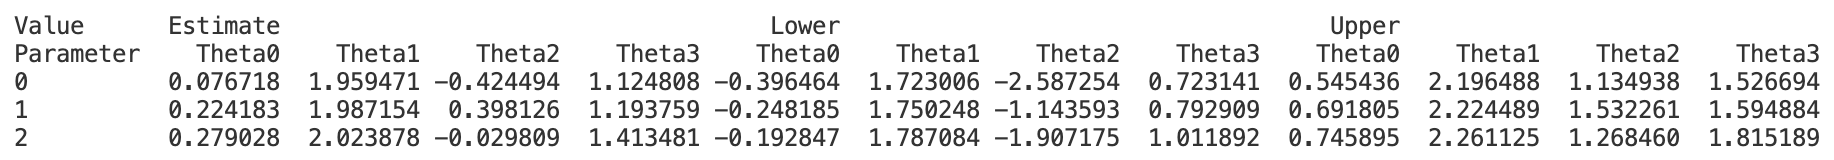
\includegraphics[scale=.5]{Images/batch_fit_frame.png}
\caption{Example dataframe returned with a batch call to the \texttt{fit()} function.}
\label{fig:batch_fit_frame}
\end{figure}

The \texttt{fit()} function can be used in batch mode by passing a list of datasets rather than a single dataframe. In this mode each dataset is fit independently yielding its own parameter estimate. This batch fitting is generally not useful for fitting to real experimental data but it is valuable for fitting to collections of simulated datasets in simulation studies. (Note, to fit multiple datasets simultaneously to achieve a single estimate, the user can simply vertically concatenate their respective dataframes and pass them as a single dataset.) Listing \ref{lst:fit_batch_fit} shows an example of a batch call with three datasets. In line 2 three datasets are simulated with a call to \texttt{sample()} and on line 4 they are bundled into a list. On line 6 options are set to return confidence intervals for each fit and on line 8 the datasets and options are passed to \texttt{fit()}. Line 10 prints the resulting dataframe containing all of the estimates and intervals. Figure \ref{fig:batch_fit_frame} shows an example of the returned dataframe from a batch call to fit. Each additional dataset adds an extra row to the returned frame. In simulation studied we are often interested in checking if true values fall in the intervals near the desired percentile rate or if the estimates exhibit a similar covariance structure to the covariance matrix predicted by the FIM. This information can easily be extracted from the returned dataframe. For example to compute the covariance of all the estimates, the user can use the expression:
\mint{python}|np.cov(fit_info['Estimate'].to_numpy().T)|
\noindent To check the fraction of datasets for which a given parameter (named \texttt{'Par'}) falls within its interval the user can call:
\begin{minted}[breaklines]{python}
sum(fit_info['Estimate','Par'].between(fit_info['Lower','Par'], fit_info['Upper','Par']))/len(fit_info)
\end{minted}

%predict paragraph
\paragraph{The \texttt{predict()} function} Generating model predictions is often the final goal of the modeling building process. However predictions are also useful during model calibration to understand expected model behaviour in various experimental scenarios as well as to understand how parameter uncertainty and sampling variability propagate to model prediction uncertainty. The \texttt{predict()} function can be used to generate model predictions for specific input settings and parameter values. The \texttt{predict()} function by default provides predictions for the mean behaviour of the observation variable, $E(Y_i)$. In addition to the mean behaviour the \texttt{predict()} function can also provide various confidence intervals for the observation variables, $Y_i$, given parameter uncertainty. This uncertainty propagation can be done using the delta method \cite{pawitan2001all} or through Monte Carlo simulation. In addition, the \texttt{predict()} function can also generate parametric sensitivities for the mean response.

\begin{figure}[htb!]
\centering
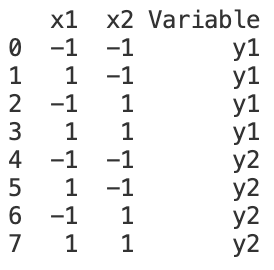
\includegraphics[scale=.7]{Images/Input_frame.png}
\caption{Example of an input dataframe used to generate predictions with the \texttt{predict()} function.}
\label{fig:predict_inputs_frame}
\end{figure}
In order to call the \texttt{predict()} function, the user must first create a dataframe containing the input and observation combinations at which they desire predictions. An example of this dataframe is shown in Figure \ref{fig:predict_inputs_frame} for a two input model with inputs names \texttt{x1} and \texttt{x2}. The last column is always named \texttt{Variable} and specifies for which observation variables predictions should be made. Here eight predictions are asked for at different input settings for one of two observation variables \texttt{y1} and \texttt{y2}.

\begin{listing}[H]
\begin{minted}[xleftmargin=\parindent,linenos,breaklines]{python}
#define the inputs for predict()
predict_inputs = pd.DataFrame({ 'x1':[-1,1,-1,1]*2,
                                'x2':[-1,-1,1,1]*2,
                               'Variable':['y1']*4 + ['y2']*4})
#specify the parameter values
params = [0.1, 2, 0.4, 1.3]
#call predict()
predictions = model_object.predict(predict_inputs, params)
#print the predictions
print(predictions)
\end{minted}
\caption{Example of a simple call to the \texttt{predict} function from the \texttt{Model} class.}
\label{lst:predict_func1}
\end{listing}

The general function call for \texttt{predict()} takes the following format;
\mint{python}|model_object.predict(input_struct, param, covariance_matrix=None, options={})|
\noindent The \texttt{input\_struct} argument accepts the previously mentioned dataframe, shown in Figure \ref{fig:predict_inputs_frame}, specifying the input and observation variables. The \texttt{param} argument accepts a list containing the parameter values at which the prediction is to be made. The \texttt{covariance\_matrix} argument is an optional argument that can be passed if the user has a parameter covariance matrix generated from an existing fit to data or a theoretical prior, this is used for computing certain prediction intervals. The \texttt{options} argument is a Python dictionary of string-value pairs that can be used to adjust default options in the prediction method, some of the more useful options are highlighted below.

\begin{figure}[htb!]
\centering
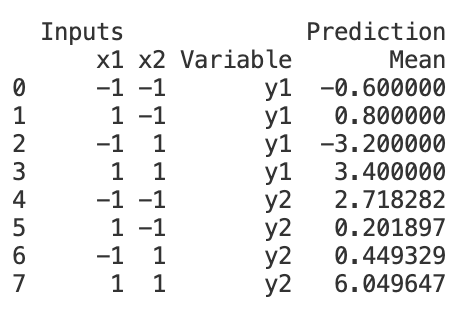
\includegraphics[scale=.7]{Images/Predict_output.png}
\caption{Example of the returned dataframe from a call to the \texttt{predict()} function.}
\label{fig:predict_ouput_frame}
\end{figure}

An example of \texttt{predict()} function call is shown in Listing \ref{lst:predict_func1}. In lines 2-4 we define the input dataframe, specifying for which inputs and observations we want predictions. In line 6 we set numerical values for the parameters and in line 8 we call the \texttt{predict()} function. In line 10 we print the predictions, the return object \texttt{predictions} is a multi-index dataframe, an example of the printed output for which is shown in Figure \ref{fig:predict_ouput_frame}. Here the columns that were passed as part of the input dataframe, specifying the inputs and observation variables, have been grouped under the upper index \texttt{Inputs}. The returned predictions for the mean response are listed under the upper index \texttt{Prediction} in the columns named \texttt{Mean}. This column lists the predicted mean observation response, $E(Y_i)$ for each condition.

\begin{listing}[H]
\begin{minted}[xleftmargin=\parindent,linenos,breaklines]{python}
#define a covariance matrix for the parameters
cov_mat = np.diag(params*0.05)
#specify desired option values
predict_opts = {'Method':'MonteCarlo',
                'PredictionInterval':True,
                'ObservationInterval':True,
                'Sensitivity':True}
#generate the predictions
predictions = model_object.predict(input_frame, params, cov_mat,predict_opts)
#display the predicted outputs
print(predictions)
\end{minted}
\caption{A more advanced example using the \texttt{predict()} function from the \texttt{Model} class to return prediction intervals and sensitivity information.}
\label{lst:predict_func2}
\end{listing}

A more advanced call to \texttt{predict()} can be used to generate intervals and sensitivity data. Listing \ref{lst:predict_func2} gives an example where the user requests both prediction and observation intervals (defined below) via Monte Carlo, as well as sensitivity data. This additional information is requested by using the \texttt{options} dictionary, see lines 4-7. Prediction intervals require the user to pass a parametric covariance matrix, which is specified in line 2 as a diagonal matrix with parameter variances set at 5\% of their nominal values. This covariance matrix defines a multivariate normal parametric prior over the parameter vector. The mean of this prior distribution is located at the parameter vector passed via the \texttt{param} argument.

Both \textit{prediction intervals} and \textit{observation intervals} are requested in Listing \ref{lst:predict_func2}. Prediction intervals are percentile-based intervals on the mean of the observation variable, $E(Y_i)$, given uncertainty in the parameters. Observation intervals are percentile-based intervals on the random observation variables, $Y_i$, itself, given both observation variability and, if a prior is provided, parameter uncertainty. For the prediction intervals, $E(y_i)$ is an expectation with respect to the observation variability of $Y_i$, and therefore the randomness inherent in each observation has been integrated out. However, the mean response, $E(Y_i)$, can still be considered random when parameter estimate uncertainty, in the form of a prior distribution, is considered. To be more precise, let the mean observation response of $Y_i$ as a function of fixed inputs and parameter values be defined as
\begin{align}
\hat{y}_i(\bm{x},\bm{\theta}) = \int_y y_i p(y_i|\bm{\eta}_i{=}\bm{f}_i(\bm{x},\bm{\theta})) dy_i.
\end{align}
Let it be emphasized that $\hat{y}_i(\bm{x},\bm{\theta})$ is a deterministic function of $\bm{x}$ and $\bm{\theta}$.
 For all of the parametric distributions used in NLOED, $\hat{y}_i(\bm{x},\bm{\theta})$ can be computed algebraically from the statistics $\bm{\eta}_i$.
 %Function attributes for computing $\hat{y}_i(\bm{x},\bm{\theta})$ are generated during instantiation of the \texttt{Model} object from the user-passed CasADi function $\bm{f}_i(\bm{x},\bm{\theta})$.
 However, when uncertainty in the parameter vector, $\bm{\theta}$, is assumed, the parametric uncertainty propagates to the mean response, $\hat{y}_i(\bm{x},\bm{\theta})$. The distribution of $\hat{y}_i(\bm{x},\bm{\theta})$ under the parameter uncertainty then depends on the prior distribution, $p(\bm{\theta})$. The \texttt{predict()} function defines the prior to be a multivariate normal distribution, centered at the value passed in argument \texttt{param} and with covariance matrix passed in argument \texttt{covariance\_matrix}. Prediction intervals are computed such that interval bounds enclose the true mean response, $\hat{y}_i(\bm{x},\bm{\theta}_o)$, of the true parameter vector, $\bm{\theta}_o$, with the prescribed confidence probability, by default 95\%. This computation obviously assumes the prior correctly reflects the uncertainty about the location of the true parameter vector. Observation intervals, on the other hand, are computed so that their bounds contain realizations, $y_i$, of the observation variable at the prescribed probability, by default 95\%. Observation intervals are computed so as to include both sampling variability, as well as parameter uncertainty if a covariance matrix has been passed. Mathematically the distribution of yet to be observed values of the observation variables, $y_i$ can be expressed as follows:
\begin{align}
p(y_i|\bm{x}) = \int_{\bm{\theta}} p_i(y_i|f_i(\bm{x},\bm{\theta}))p(\bm{\theta}) d\theta.
\end{align}
The observation interval bounds are determined from the percentiles of this distribution. Without parameter uncertainty this distribution just reduces to the observation distribution $p_i(y_i|\bm{f}_i(\bm{x},\bm{\theta}))$.  

An example of the returned \texttt{predictions} dataframe from Listing \ref{lst:predict_func2}, containing both types of intervals and sensitivity data, is shown in Figure \ref{fig:predict_advanced_return}. Several additional columns are now included, grouped by upper indices. The upper index \texttt{Prediction} now includes columns \texttt{Lower} and \texttt{Upper} which mark the lower and upper bounds of the prediction interval for each input-observation combination. A new upper index \texttt{Observation} has been added, containing \texttt{Lower} and \texttt{Upper} bound columns for the 95\% observation intervals. Note that under parameter uncertainty the predicted mean response, $E_{\bm{\theta}}(\hat{y}_i)$, and the mean observation, $E_{y,\bm{\theta}}(y_i)$, should be the same and so only the predicted mean is returned (i.e. $E_{\bm{\theta}}(\hat{y}_i)$). Sensitivities of the prediction mean (taken at the value passed via the \texttt{param} argument) are shown in the third upper index grouping named \texttt{Sensitivities}. Here each column is named according to the parameter names the user originally passed to the \texttt{Model} class during instantiation.
%-Should maybe change name prediction, to expectation??
\begin{figure}[htb!]
\centering
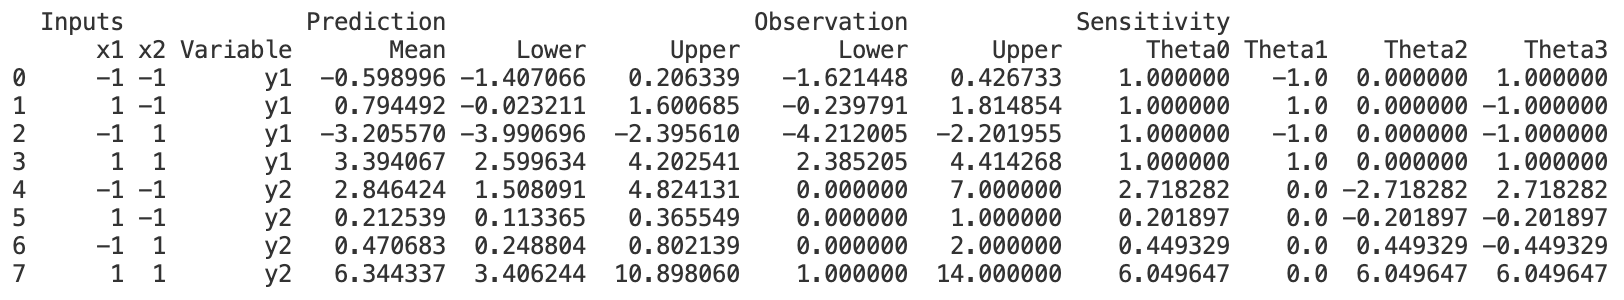
\includegraphics[scale=.56]{Images/Adv_predict_output.png}
\caption{An example of the returned dataframe from the \texttt{predict()} function, including prediction and observation intervals as well as sensitivity information.}
\label{fig:predict_advanced_return}
\end{figure}

When computing the mean response, prediction intervals, and observation intervals, the user has a choice of method options: \texttt{Exact}, \texttt{Delta} and \texttt{MonteCarlo}. Only one method can be used in a given call to \texttt{predict()}, and all returned information will be computed using the selected method. The \texttt{Exact} method is the default method, and it ignores any parameter uncertainty. The \texttt{Exact} method returns $E(Y_i)$ computed algebraically from the statistics, $\bm{\eta}_i$, computed at the nominal parameter values passed. The \texttt{Exact} method cannot compute prediction intervals as the propagation of a normal prior through a non-linear model cannot be computed exactly, at least for arbitrary models. The observation intervals can be computed exactly, ignoring any parameter uncertainty, by using the cumulative distributions function of the observation probability distribution, $p_i(y_i|\bm{f}_i(\bm{x},\bm{\theta}))$. The \texttt{Delta} method propagates parameter uncertainty using local parametric sensitivities and a normal approximations for the prediction and observation intervals \cite{pawitan2001all}. Using the \texttt{Delta} method, the \texttt{predict()} function can compute mean, prediction intervals, and observation intervals, but these may be inaccurate for observation distributions that are not well approximated by the normal distribution and for highly nonlinear models. For example, due to the normal approximation in the \texttt{Delta} method, interval bounds can be negative even if the observation variable is strictly positive. The \texttt{MonteCarlo} method uses Monte Carlo sampling from the parameter prior, $p(\bm{\theta})$, and the observation distribution, $p_i(y_i|\bm{f}_i(\bm{x},\bm{\theta}))$, to compute the mean response and intervals. The Monte Carlo method can be accurate for most scenarios but can be slow and may require the user to increase the default number of samples via the options dictionary to ensure stable estimates. 

%Do we have a batch call for fitting to multiple datasets and getting single overall param est (guess its just concat datasets together) should note this in text

% User callable/Output stuff
% \begin{itemize}
%   \item Predict
%   \subitem prediction intervals; delta/MC CI's
%   \subitem item sensitivity 
%   \item Sample (batch etc.)
%   \item Fit
%   \subitem profile liklihoods and confidence regions
%   \item Evaluate
%   \subitem Asymptotic vs Monte Carlo features
% \end{itemize}

% screen shots of data frames for designs predictions etc.

\section{The \texttt{Design} Class}

%\textbf{This section introduce the Design class, which is used for generating optimal design. We give a brief outline of its role in the package. We the discus figure \ref{fig:Design_Class}, walking the reader through 1) the objects creation (and the data needed for that), 2) through the internal automatic processes, 3) then to the user-callable functions that the user can use at the end. Each of the following subsections will discuss these in detail.}

The \texttt{Design} class is used to generate optimal designs in the NLOED package. Design optimization is conditional on the model and parameter values at which the design is optimized, but also depends on experimental constraints encoded in the optimization, and on how the optimization problem is structured computationally. Each of these factors can alter the resulting optimal design structure. Therefore it may often be the case that the user will want to create multiple optimal designs under various scenarios, and then compare their performance. This motivates having designs encapsulated in a specific class object, so that multiple designs can be created in a modular fashion by instantiating a \texttt{Design} object for each scenario the user wishes to consider. Another reason for having designs encapsulated in a \texttt{Design} object, is that the output of any design optimization problem in NLOED is a relaxed design which requires additional processing to generate an exact design. This processing is not necessarily unique and involves some user choices. The \texttt{Design} class therefore stores relaxed solutions internally and provides users an easy functional interface to generate various exact designs from the relaxed solution. 

\begin{figure}[htb!]
\centering
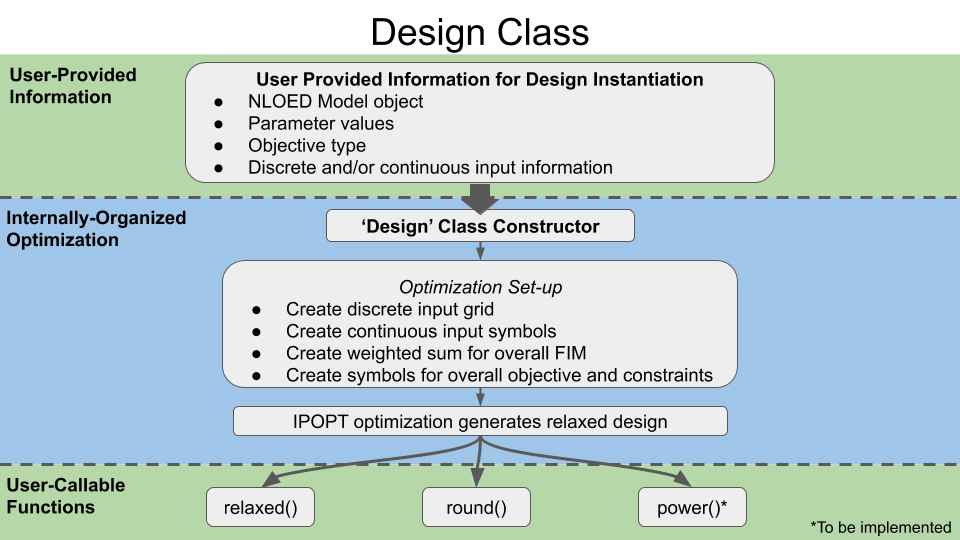
\includegraphics[scale=.4]{Images/DesignClass.png}
\caption{Caption text}
\label{fig:Design_Class}
\end{figure}

Figure \ref{fig:Design_Class} outlines the basic process for creating a \texttt{Design} object. Here, as in Figure \ref{fig:model_class}, the green areas indicate user-controlled passing of data or calling of functions. The blue area indicates automatic processes performed during object instantiation. The upper green area is labelled as \textit{User Provided Information}, this area indicates the various data and options the user needs to provide to the \texttt{Design} class constructor for object creation. This information includes which model and parameter value are going to be used, as well as which objective is optimized, how each input variable is to be handled by the optimization algorithm, and choices about sampling flexibility for models with multiple observation variables. Together this information determines the exact nature of the optimization problem and will influence the resulting design considerably. Once this information is properly encoded and passed to the class constructor, instantiation of the \text{Design} object commences. 

Instantiation of the \texttt{Design} class will only take a single line of code to initiate, but as the instantiation process contains a call to IPOPT for optimization, this can take some time to complete. During this process several automated actions are taken within the \texttt{Design} class constructor. These automated processes are labelled as \textit{Internally-Organized Optimization} in Figure \ref{fig:Design_Class}. These processes are primarily split into two parts, 1) optimization set-up and 2) the IPOPT call for optimization that generates the relaxed design. During optimization set-up the specific information passed during instantiation, especially function attributes within the passed models, are used to construct a CasADi symbol for the optimization problem and its constraints. Once this symbolic structure is prepared, it is passed to IPOPT via CasADi's interface; the optimizer then runs and returns an optimal solution which is parsed and stored within the resulting design object. 

After optimization completes, the design object will be fully instantiated and the user can interact with it using various user-callable functions. These are shown in the bottom green section and are labeled \textit{User-Callable Functions} in Figure \ref{fig:Design_Class}. These functions can be used to create exact designs from the optimal relaxed archetype or to compare various exact designs' performance depending on user's choice regarding the sample size. Specifically, the \texttt{round()} function can be used to return an exact design as a dataframes in NLOED's default design format. The exact designs can be used directly with the \texttt{Model} class's user-callable functions like \texttt{sample()} and \texttt{evaluate()} for further analysis, or to guide real experimentation. The following subsections give detailed descriptions of each of the three phases outlined in Figure \ref{fig:Design_Class}, including sample code and call structures where appropriate.

\subsection{Creating a \texttt{Design} Object}

%\textbf{This subsection explains how to create a Design object. It gives sample code, explains the various input choices and how the design problem is posed. It also discusses different objects (i.e. a Model class object) that need to be created before hand to create a Design object. }
In order to create a \texttt{Design} object the user needs to call the \texttt{Design} constructor. The general call structure for the \texttt{Design} class constructor is;
%\mint{python}|Design(models, parameters, objective, discrete_inputs=None, continuous_inputs=None, observ_groups=None, fixed_design=None, options={})|
\begin{minted}[breaklines]{python}
Design(models, parameters, objective, discrete_inputs=None, continuous_inputs=None, observ_groups=None, fixed_design=None, options={})
\end{minted}
The first three arguments; \texttt{models}, \texttt{parameters}, and \texttt{objective} are always required. The \texttt{models}, argument accepts a model object of the \texttt{Model} class created previously by the user. 
%BPI, NEED TO SEPARATE FUTURE FROM CURRENT SOMEHOW
 %The \texttt{models} argument accept a \texttt{Model} instance for which an optimal design is desired.
 %In the current implementation, the \texttt{models} argument can also accept a list of \texttt{Model} instances as along as they have the same input structure.With a list of \texttt{Model} instances passed, the design is then optimized for the mean objective value of each model. This feature ensures robustness across model uncertainty, however it is still being tested and its use is not fully described  here. 
 The \texttt{parameters} argument accepts a the nominal parameter values at which the optimal design is computed. %In future releases, this local analysis will also be supplemented with pseudo-Baysian methods which allow for design optimization over a weighted average of several candidate parameter points \cite{schenkendorf2009optimal}.
%In future releases, this local analysis will also be supplemented by allowing \texttt{parameters} to also accept either mean and covaraiance information for a normal prior, or a list of equally-likely candidate parameter values. Averaged optimal designs can then be generated with respect to the given parameter uncertainty by using the sigma-point method \cite{schenkendorf2009optimal} or related approaches  -- these features are also still in development. 
The \texttt{objective} argument accepts a string specifying the objective function type. Currently this argument only accepts \texttt{D} for D-optimal designs (the determinant of the Fisher information matrix). %Other objectives will be added in future releases.
%In future releases this argument will accept other FIM based objectives such as D$_s$-optimal and A-optimal objectives. Each of these prospective features are near completion and expected to be included in the initial release.

The remaining input arguments: \texttt{discrete\_inputs}, \texttt{continuous\_inputs}, \texttt{observ\_groups}, \texttt{fixed\_design}, and \texttt{options}, are optional to varying degrees. The user exerts significant control over the posing of the design problem in specifying these remaining arguments. The \texttt{discrete\_inputs} and \texttt{continuous\_inputs} arguments control how the inputs to the model are handled. 
%Both \texttt{discrete\_inputs} and \texttt{continuous\_inputs} are Python dictionaries with multiple possible key-value fields controlling the \texttt{Design} constructor handles the various model inputs during design optimization.
%These arguments allow the user to trade computational costs against degrees of approximation for a given design problem. 
At least one of these two input-related arguments must be passed, as all inputs must be treated as either discrete or continuous. 
%The user uses these two arguments to partitions all the inputs of a model into one of the two types; \textit{discrete} and \textit{continuous}.
Discrete inputs are dimensions for which the optimization algorithm will only consider discrete levels of the input in the design. Continuous inputs are treated as real-valued and thus can be varied accordingly.
The \texttt{observ\_groups} argument accepts information about which observation variables must be sampled together. By default the \texttt{Design} class assumes all observations can be replicated with complete flexibility and independence, sometimes this is not possible and \texttt{observ\_groups} allows the user to force additional structure on which observation variables can be measured together in a given input condition. The argument \texttt{fixed\_design} allows the user to pass an existing fixed design to the \texttt{Design} class. This is useful if the user has certain observations that need to be taken regardless of the optimal design (i.e. based on domain specific knowledge) or to optimize the current design conditionally on past data. The \texttt{options} arguments is optional and accepts a dictionary of key-value pairs to modify default settings of the \texttt{Design} constructor and optimization. 

%BPI; BRIAN SAYS THIS IS HARD TO READ, MAYBE ORGANIZE BY SUBHEADING RATHER THAN INLINE PARAGRAPHS
To help explain the behaviour of the optional arguments of the \texttt{Design} constructor, assume an existing model object, \texttt{model\_object}, has been passed to the \texttt{Design} constructor. Also assume that \texttt{model\_object} has four inputs, and two observation variables. Let the input names be: \texttt{x1}, \texttt{x2}, \texttt{x3}, and \texttt{x4}
%; the parameter names be: `\texttt{Par1}', `\texttt{Par2}', `\texttt{Par3}', and `\texttt{Par4}'
, and the observation variable names be: \texttt{y1} and \texttt{y2}. In the subsequent paragraphs this example model will be used to explain the usage of the various optional arguments. As the descriptions are quite lengthy, the topics are outlined here for clarity:
\begin{itemize}
    \item \textbf{Discrete Inputs} Using the \texttt{discrete\_inputs} argument to handle all model inputs.
    \item \textbf{Continuous Inputs} Using the \texttt{continuous\_inputs} argument to handle all model inputs.
    \item \textbf{Mixed Inputs} Using a both the \texttt{discrete\_inputs} and \texttt{continuous\_inputs} argument to handle different model input subsets as either discrete or continuous.
    \item \textbf{Observation Groups} Using the \texttt{observ\_groups} argument to force observation variables to be sampled together. 
    \item \textbf{Fixed Design Aspects} Using the \texttt{fixed\_design} argument to pass in an existing or fixed aspect of the experimental design for conditional optimization.
\end{itemize}

\paragraph{Discrete Inputs}  Both the \texttt{discrete\_inputs} and \texttt{continuous\_inputs} arguments are dictionaries, each with multiple fields. The user must create them prior to passing them to the \texttt{Design} constructor. To assign all four inputs to be discrete, the user can use the code in Listing \ref{lst:discreet_only}.
\begin{listing}[H]
\begin{minted}[xleftmargin=\parindent,linenos,breaklines]{python}
#discrete_input argument creation
discrete_dict ={'Inputs':['x1','x2','x3','x4'],
                'Grid':[[-1,-3,-6,3],[0,0,0,0],[4,1,2,-1],
                        [3,8,-3,7],[9,7,-7,9],[0.1,0.3,-0.2,1]]}
#declare parameters
param = [2, 3.3, 0.5, 1]
#call Design constructor
design_object = Design(model_object, param, 'D', discrete_inputs=discrete_dict)
\end{minted}
\caption{Example of the \texttt{discrete\_inputs} argument creation and passage, assigning four model inputs to be handled discretely.}
\label{lst:discreet_only}
\end{listing}
\noindent The \texttt{Inputs} key must be passed for \texttt{discrete\_inputs}, its value is a list of strings naming the inputs to be treated discretely. Here all inputs are listed in the \texttt{Inputs} field of the dictionary, which means all inputs are handled discretely and the \texttt{continuous\_inputs} argument can be ignored. When inputs are discretized the optimization algorithm only considers discrete levels of each input, permuted to create a grid of candidate input points in the discrete input domain. The remaining keys in \texttt{discrete\_inputs} determine the layout of the discrete grid for the specified inputs. The user can specify the grid in three ways; 1) with \texttt{Grid} key, 2) with the \texttt{Candidates} key, and 3) with the \texttt{Bounds} and \texttt{NumPoints} keys. As shown in Listing \ref{lst:discreet_only}, the user can specify the exact set of grid points using the \texttt{Grid} key, which is followed by a list of lists; the outer list contains all of the grid points, the inner list specifies the input values at each point. Values in the inner lists are assumed to be ordered in the same way the discrete input names were passed via the \texttt{Inputs} key. Passing the exact set of grid points gives the user complete control over which input combinations are considered, but it can be time consuming to construct. In the case where the user requires specific discrete levels of each input to be considered but faces no other limitation, they can use the \texttt{Candidates} key. Here the user passes a list of lists again, but the outer list is the same length as the number of discrete inputs. Each inner list contains the unique candidate values of the corresponding input to be consider. The inner lists can be of different lengths. An example of this type of dictionary is shown below:
\begin{minted}[xleftmargin=\parindent,breaklines]{python}
#discrete input argument creation
discrete_dict ={'Inputs':['x1','x2','x3','x4'],
                'Candidates':[[-1,0,1],
                              [1,5,10,15,20],
                              [.1,.7,12,200]],
                              [0,1,2,3,4,5,6,7,8,9,10]}
\end{minted}
 The \texttt{Design} constructor will generate all possible permutations of the provided candidate lists and use this permutation set as the grid of potential input points. Finally, in some experiments the user may wish to simply distribute points evenly through some region of the discrete input space. To do so they can use the \texttt{Bounds} and \texttt{NumPoints} keys. When passing the \texttt{Bounds} key, the user gives the lower and upper bounds for each discrete input dimension as a list of tuples. The \texttt{Design} constructor then creates a grid of candidate points in this hyper-rectangle defined by the bounds, with the integer passed via the \texttt{NumPoints} key determining the number of points per dimension. The points within each dimension are distributed in an equidistant manner and all permutations within the hyper-rectangle defined by the bounds are considered. If \texttt{NumPoints} is not passed, the number of values along each dimension defaults to 5. The \texttt{Bounds} and \texttt{NumPoints} keys are useful for quickly generating an equidistant candidate grid if the exact value of the discrete levels do not matter. 
 %this should maybe allow for different number of points per dimension...
An example dictionary using the \texttt{Bounds} and \texttt{NumPoints} keys is given below:
\begin{minted}[xleftmargin=\parindent,breaklines]{python}
#discreet input argument creation
discrete_dict = {'Inputs':['x1','x2','x3','x4'],
                 'Bounds':[(-1,1),(-1,1),(-1,1),(-1,1)],
                 'NumPoints':10}
\end{minted}

There are a number of reasons the user would consider using discrete inputs. Real experimental inputs to a system, when implemented in the lab, are always restricted to discretely distinguished levels by experimental measurement accuracy and equipment limitations. Even if an input such as temperature could in theory be resolved down to an infinitesimal scale, an experimental apparatus in the lab can only maintain temperature consistently in a bounded range, determined by measurement accuracy and the apparatus control resolution. Some experimental inputs cannot be varied from a few discrete levels (i.e. growth rate on various carbon sources), and some inputs are simply numerical encodings of categorical factors that have no ordering (i.e. background strain, antibiotic type etc.). In certain models it can be advantageous to discretize an input, despite its fine experimental resolution, either because the model is relatively insensitive to the given input or greater optimization efficiency can be achieved via discretization. Discrete inputs impose a higher upfront computational cost and a create a larger overall optimization problem (with higher memory overhead) but discretization leads to faster iterations of the optimization solver due to increased convexity and a simpler overall problem structure. The problem size and upfront cost scale with the number of discrete candidate points considered in the input space. As the grid generally grows exponentially with the number of input dimensions, it is generally difficult to handle high-dimensional problems with all inputs treated discretely. 

\paragraph{Continuous Inputs} In order to treat inputs continuously the user passes the \texttt{continuous\_inputs} argument, which accepts a dictionary with somewhat similar structure to its discrete counterpart, \texttt{discrete\_inputs}. An example of a call to the \texttt{Design} constructor with all inputs treated continuously is shown in Listing \ref{lst:continuous_only};
\begin{listing}[H]
\begin{minted}[xleftmargin=\parindent,linenos,breaklines]{python}
#continuous input argument creation
continuous_dict = {'Inputs':['x1','x2','x3','x4'],
                   'Bounds':[(-1,1),(-1,1),(-1,1)],
                   'Structure':[['x1_lvl1','x2_lvl1','x3_lvl1','x4_lvl1'],
                               ['x1_lvl2','x2_lvl2','x3_lvl2','x4_lvl2'],
                               ['x1_lvl3','x2_lvl3','x3_lvl3','x4_lvl3']]}
#declare parameters
param = [2, 3.3, 0.5, 1]
#call Design constructor
design_object = Design(model_object, param, 'D', continuous_inputs=continuous_dict)
\end{minted}
\caption{Example of the \texttt{continuous\_inputs} argument creation and passage, assigning four model inputs to be handled continuously.}
\label{lst:continuous_only}
\end{listing}
\noindent Here, the \texttt{Inputs} key maps to a list of input names that are to be treated continuously. In Listing \ref{lst:continuous_only}, all four inputs are listed in the \texttt{Inputs} field of \texttt{continuous\_dict} and so the \texttt{discrete\_inputs} argument can be ignored. Similar to the discrete case, the \texttt{Bounds} key for continuous inputs are also specified as a list of tuples containing lower and upper bounds for each input. All continuous inputs must have boundaries specified. These input bounds are necessary as they ensure well-posedness of the optimization problem; the objective value can increase indefinitely with the increase of some combinations of input dimensions for certain models. Also, it is generally infeasible or impractical to vary the input values beyond some natural limits within the laboratory. Bounds can be imposed based on limitations of experimental equipment or based on restrictions on the input ranges for which the model assumptions hold. When discrete inputs are used, the candidate grid points are fixed and the optimization selects inputs by adding them to the solution based on their utility. When using continuous inputs, the input points are treated as the optimization variable themselves, and the user must specify how many unique points the optimizer should consider within the bounded input space. The \texttt{Structure} key allows the user to specify how many unique input points to consider and any common dimensional values they may need to share. The \texttt{Structure} key must be passed with a list of lists as its value. The outer list corresponds to the number of unique input points that will be considered in the continuous input space. Each inner list has the same number of dimensions as the number of continuous inputs. The inner lists each contain a set of string symbols, one for each continuous input dimension. Each unique string symbols specifies a unique level for the corresponding continuous input.

In the example shown in Listing \ref{lst:continuous_only}, we have specified three unique points in the continuous input space; each point has complete freedom in each of the four input dimensions. This scenario is encoded with three inner lists, one for each point. The independence of every point and dimension is indicated by the use of a novel symbol string for every list entry (i.e. `\texttt{x1\_lvl1}', `\texttt{x2\_lvl2}', etc.). However using the \texttt{Structure} key we can also specify more constrained experimental design problems. For example, we may consider six input points, but for all six, \texttt{x1} can only have one unique value. We may also wish to restrict input \texttt{x2} to one level in the first three points and another in the later three points. Inputs \texttt{x3} and \texttt{x4} are assumed to be free in all six input points. An example of the \texttt{continuous\_inputs} dictionary encoding such restrictions is shown in Listing \ref{lst:continuous_restrict}.
\begin{listing}[H]
\begin{minted}[xleftmargin=\parindent,breaklines]{python}
#continuous input argument creation
continuous_dict = {'Inputs':['x1','x2','x3','x4'],
                   'Bounds':[(-1,1),(-1,1),(-1,1),(-1,1)],
                   'Structure':[['x1_lvl','x2_lvl1','x3_lvl1','x4_lvl1'],
                                ['x1_lvl','x2_lvl1','x3_lvl2','x4_lvl2'],
                                ['x1_lvl','x2_lvl1','x3_lvl3','x4_lvl3'],
                                ['x1_lvl','x2_lvl2','x3_lvl4','x4_lvl4'],
                                ['x1_lvl','x2_lvl2','x3_lvl5','x4_lvl5'],
                                ['x1_lvl','x2_lvl2','x3_lvl6','x4_lvl6']]}
\end{minted}
\caption{Example of the \texttt{continuous\_inputs} argument that uses the \texttt{Structure} field to encode candidate points with shared dimensional values.}
\label{lst:continuous_restrict}
\end{listing}
\noindent Note how the first element of each inner list is now the same string; `\texttt{x1\_lvl}', indicating that input \texttt{x1} has a single value, shared across all points to be optimized. The second element of each inner list is either `\texttt{x2\_lvl1}' (in the first three) or `\texttt{x2\_lvl2}' (in the latter three), indicting input \texttt{x2} will only take two unique values after optimization. Lastly, every element corresponding to inputs \texttt{x3} and \texttt{x4} has a unique string, indicating unique levels for each point.

The \texttt{Structure} field will often be used as shown in Listing \ref{lst:continuous_only}, with all points free, and the main choice being how many inputs points to consider. However the more complicated points structure shown in Listing \ref{lst:continuous_restrict} are required in certain experiments. For example consider a time series experiment where the initial conditions are a model input and all replicates share the same initial conditions. In such a case, the initial condition input will need to be restricted to a single value for all replicates, just like \texttt{x1} above. Another example may be that limited capacity of a laboratory, like the number of incubators, may necessitate certain input dimensions, such as temperate, can only take a finite number of unique values in each experiment, just like input \texttt{x2} above only has two levels. 

When using continuous inputs, the \texttt{Design} constructor will optimize the placement of the input points and will also attempt to optimize the quantity of replicates taken at each point (this is also done for discrete inputs). However for continuous inputs the user may wish to specify that each input point in the structure gets exactly the same number of observations. This option is ideal for optimizing design with smaller sample sizes. To do so the user can pass the option '\texttt{LockWeights}' as \texttt{True} in the \texttt{options} argument. This option is only available if all inputs are handled continuously.

Choosing to treat inputs continuously rather than discretely depends on the model and the experimental context. Generally, real world experimental levels are discrete up to the tolerance of measurement and control, and thus continuous inputs are an approximation. However, it is generally practical to approximate inputs as continuous if the number of discrete levels achievable in the laboratory is numerous and the experimental control is very fine relative to the model's input sensitivity. Continuous inputs can also be used for computational reasons as they generally lead to smaller problems that are quick to initialize. However continuous inputs generally result in an optimization problem that is more nonlinear leading to more optimizer iterations, more intensive computation on each iteration, and greater chances of getting stuck in local optima. In addition for continuous inputs, the user needs to specify the number of unique input points the algorithm should consider in the design; this information can be difficult to set \textit{a priori}. 

\paragraph{Mixed Inputs} In certain situations it is desirable to handle some inputs discretely while treating others as being continuous. This can be for both experimental or computational considerations. For example, adding some discrete inputs tends to make a design problem more convex and easier to solve, but adding some continuous inputs can make the overall problem smaller with respect to memory requirements. When dealing with very complex models or input spaces, blending the input types can allow the user to tackle problems that may be difficult to handle with a single input type. Listing \ref{lst:mixed_inputs} shows an example where input \texttt{x1} and \texttt{x2} have been handled continuously, with similar restrictions to those imposed in Listing \ref{lst:continuous_restrict}. Inputs \texttt{x3} and \texttt{x4} have been discretized. In this case both the \texttt{discrete\_inputs} and \texttt{continuous\_inputs} arguments are passed, with the model's four inputs split between both input structures.
\begin{listing}[H]
\begin{minted}[xleftmargin=\parindent,linenos,breaklines]{python}
#continuous input argument creation
continuous_dict = {'Inputs':['x1','x2'],
                   'Bounds':[(-1,1),(-1,1)],
                   'Structure':[['x1_lvl','x2_lvl1'],
                                ['x1_lvl','x2_lvl1'],
                                ['x1_lvl','x2_lvl1'],
                                ['x1_lvl','x2_lvl2'],
                                ['x1_lvl','x2_lvl2'],
                                ['x1_lvl','x2_lvl2']]}
#discrete input argument creation
discrete_dict ={'Inputs':['x3','x4'],
                'Candidates':[[-1,-.5,0,.5,1],
                              [-1,-.5,0,.5,1]]}
#declare parameters
param = [2, 3.3, 0.5, 1]
#call Design constructor
design_object = Design(model_object, param, 'D', discrete_inputs=discrete_dict,continuous_inputs=continuous_dict)
\end{minted}
\caption{Example calling the \texttt{Design} constructor using a mixture of discrete and continuous inputs.}
\label{lst:mixed_inputs}
\end{listing}

\paragraph{Observation Groups} The \texttt{observ\_groups} argument to the \texttt{Design} constructor is optional. By default each observation variable is handled independently meaning that during optimization, outputs \texttt{y1} and \texttt{y2} could have different replicate quantities assigned to them even in the same input conditions. In certain conditions this is not practical, for example in a costly destructive sampling experiment where a replicate is destroyed on observation. In this case the user will likely measure any relevant observation variables they are able to whenever a replicate is destroyed. In this case it is useful to assign the relevant observation variables to a group that will be sampled together. The \texttt{observ\_groups} argument accepts a list of lists, each inner list contains the names of observation variables that are measured in an observation group. For example if \texttt{y1} and \texttt{y2} needed to be measured together in any observation, one could use the example shown in code listing
\ref{lst:observe_struct}.
\begin{listing}[H]
\begin{minted}[xleftmargin=\parindent,linenos,breaklines]{python}
#discreet input argument creation
discrete_dict = {'Inputs':['x1','x2','x3','x4'],
                 'Bounds':[(-3,3),(-3,3),(-3,3),(-3,3)],
                 'NumPoints:10}
#declare parameters
param = [2, 3.3, 0.5, 1]
#observation grouping
observ_group_lst = [['y1','y2']]
#call Design constructor
design_object = Design(model_object, param, 'D', discrete_inputs=discrete_dict, observ_groups = observ_group_lst)
\end{minted}
\caption{Example of the \texttt{observ\_groups} argument being used to group observation variables \texttt{y1} and \texttt{y2}.}
\label{lst:observe_struct}
\end{listing}
\noindent The \texttt{observ\_groups} list is constructed in line 8 and is passed in line 10. This will force both observations \texttt{y1} and \texttt{y2} to be treated as a single unit when the algorithm considers the number of samples to assign to them. %In future release this argument will also be able to handle observations that must not be made 

\paragraph{Fixed Design Aspects} The \texttt{fixed\_design} argument is also optional and can be used to pass fixed design aspects or the design used in existing data. The \texttt{fixed\_design} argument accepts a dictionary containing an existing design along with a weight indicating what fraction of the overall sample size dedicated to the fixed design aspects. For example if the user has already collected 5 observations and plans to collect another 15 with an optimal design, the user would pass the \texttt{fixed\_design} argument with a weight of 0.25. A coded example using the \texttt{fixed\_design} argument is shown in Listing \ref{lst:fixed_design}. Here in lines 6-11, the initial design is declared. In practice this design can come from a previous optimal design or past datasets. In line 13 the initial design is inserted into a dictionary under the key name \texttt{Design}. In the same dictionary we also include the key name \texttt{Weight} whose value specifies the fraction (between 0 and 1) of the overall sample size dedicated to the initial design. In this case the value of 0.25 is passed as the weight and so the designed experiment is expected to have a sample size three times that of the initial experiment. Passing in fixed aspects of an overall experimental effort is important in order for the optimal design to perform well. Optimal designs created without conditioning on fixed design aspects will ignore information contained in the fixed aspects. This may lead to some observations in the optimal design being inefficiently placed. 

\begin{listing}[H]
\begin{minted}[xleftmargin=\parindent,linenos,breaklines]{python}
#discrete input argument creation
discrete_dict = {'Inputs':['x1','x2','x3','x4'],
                 'Bounds':[(-3,3),(-3,3),(-3,3),(-3,3)],
                 'NumPoints:10}
#declare initial design
init_design = pd.DataFrame({'x1':[-2,-1,1,2]*4,
                            'x2':[2,-2,-1,1]*4,
                            'x3':[1,2-2,-1]*4,
                            'x4':[-1,1,2,-2]*4,
                            'Variable':['y1']*4+['y2']*4,
                            'replicates':[3]*8}) 
#create the fixed design dictionary
fixed_dict = {'Weight':0.25,'Design':init_design}
#declare parameters
param = [2, 3.3, 0.5, 1]
#observation grouping
observ_group_lst = [['y1','y2']]
#call Design constructor
design_object = Design(model_object, param, 'D', discrete_inputs=discrete_inputs, fixed_design = fixed_dict)
\end{minted}
\caption{Example of a call to the \texttt{Design} constructor with the \texttt{fixed\_design} argument used to pass an existing aspect of the overall design.}
\label{lst:fixed_design}
\end{listing}

%\texttt{options} Should may discuss options here.

% \begin{itemize}
%   \item List of models
%   \item Prior information or fixed portion of the design
%   \item Input constraints, mixed input structure
% \end{itemize}

% \begin{itemize}
%   \item Basic inputs to model class:
%   \subitem Model instance
%   \subitem Parameter values
%   \subitem Objective
%   \subitem Input ranges and whether they are handled discreetly or continuously 
%   \item Additional controls
%   \subitem List of models
%   \subitem Prior information or fixed portion of the design
%   \subitem Continuous input archetype structure
%   \subitem Discrete input, user provided candidate grid or auto-generation
%   \subitem Input constraints, mixed input structure
%   \subitem Observation structure; fixed co-observation eg, mrna and prot, or dynamic experiments where all time points must be taken
% \end{itemize}

\subsection{\texttt{Design}'s Automatic Optimization Set-up}

%\textbf{This subsection discusses what happens internally after the user actually runs the line of code that creates a Design object. All of this happens automatically so the goal is to give a high-level understanding of what the Design class does to set up the optimization problem. We may borrow some graphics from the SIAM slides showing different FIMs being added and weighted.}


After the \texttt{Design} constructor is called, instantiation of the \texttt{Design} object begins with the automatic organization the optimization problem for passage to IPOPT. The main challenge in setting up the optimization problem is in creating the CasADi symbol for the overall design objective. In order to create the objective symbol, the optimization variables need to be linked to the total Fisher information matrix for the experiment. All objectives used by the NLOED package for optimization are computed as simple algebraic functions from the elements of the experiment's Fisher information matrix; computing the total FIM for a design is therefore the main computational hurdle. %For example the default D-optimal objective is equivalent to maximizing the determinant of the Fisher information matrix computed across all of the observations.

As observations in NLOED are assumed to be independent, the Fisher information matrix for an experiment can be computed as a weighted sum of individual matrices at each observation. For a multi-output model the FIM sum can be written as (see Chapter \ref{background_chapter} for details)
\begin{align}
I_{Tot}(\mathcal{D},\bar{\bm{\theta}}) = \sum_j^N \sum_i^M \beta_{i,j} I_i(\bm{x}_j,\bar{\bm{\theta}}).
\end{align}
Here there are $M$ observation variables, $Y_i$, indexed by $i$, and $N$ support points $\bm{x}_j$, indexed by $j$. The support of the design consists of the set of all unique input vectors such that $\bm{x}_j\in\mathcal{X}$. The FIM at a given input point, $\bm{x}_j$, for the observation variable $Y_i$ is $\mathcal{I}_j(\bm{x}_i,\bar{\bm{\theta}})$. The vector $\bar{\bm{\theta}}$ is the nominal parameter vector at which the design is optimized. Each replicate allocation, $\beta_{i,j}$, corresponds to a support point $\bm{x}_j$ and an observation variable $Y_i$. Together the replicate allocations for each observation and input condition form the set $\beta_{i,j}\in\mathcal{B}$, which defines the design's replication structure. For an exact design the weights are restricted to be non-negative integers. The sum of the weights adds to the overall sample size $N_{Tot}$ such that; $N=\sum_i^{M}\sum_j^{N}\beta_{i,j}$. The overall information matrix, $\mathcal{I}_{Tot} (\mathcal{D},\bar{\bm{\theta}})$, is therefore a function of the design, $\mathcal{D} $, where the design consists of the support point set, $\mathcal{D}$, and weight set, $\mathcal{B}$, such that; $\mathcal{D} =\{\mathcal{X},\mathcal{B}\}$. The integer constraint makes the above problem very difficult. In the \texttt{Design} class the integer constraint on the replicates is relaxed, and the integer replicate allocations, $\beta_{i,j}$, are replaced with real-valued continuous weights, $\xi_{i,j}$, which are constrained so that $1=\sum_i^{M}\sum_j^{N}\xi_{i,j}$. The relaxed design problem can then be written as
\begin{align}
I_{Tot}(\mathcal{D}_R,\bar{\bm{\theta}}) = \sum_j^N \sum_i^M \xi_{i,j} I_i(\bm{x}_j,\bar{\bm{\theta}}).
\end{align}
For the relaxed formulation, all the weights, $\xi_{i,j}$, now form the weight set $\xi_{i,j}\in\mathcal{Z}$, and the relaxed design is defined as $\mathcal{D}_R =\{\mathcal{X},\mathcal{Z}\}$. The problem in the relaxed form remains nonlinear but it is now possible to pass to a solver such as IPOPT and expect reasonable solution times for many models of interest. %That said, this approximation is already layered ontop of the significant approximations to the parameter fit distribution assumed by using the FIM as the objective in the first place.  FIM is only an asymptotic expectation at first order for a random vector.)

%BPI; ADD EQUATION NUMBERS AND REFER IN TEXT WHERE NEEDED, ESPECIALLY HERE (I.E. 'ABOVE')
In order to compute the FIM sum for a given experiment, the \texttt{Design} constructor uses the FIM function attributes of the \texttt{Model} object passed to the \texttt{Design} constructor. These function attributes are able to compute $\mathcal{I}_i(\bm{x}_j,\bar{\bm{\theta}})$ and can therefore compute the individual FIM's symbolic dependence on each of the candidate support points. The total FIM sum, listed previously, is generated as a CasADi symbolic function with $\xi_{i,j}$ and $\bm{x}_j$ as the symbolic inputs.  The total FIM is then used to generated a CasADi symbol for the overall optimization objective symbol, $\Psi(I_{Tot}(\mathcal{D}_R,\bar{\bm{\theta}}))$. The resulting objective symbol, $\Psi(I_{Tot}(\mathcal{D}_R,\bar{\bm{\theta}}))$, effectively encodes the entire optimization problem in a CasADi symbolic structure, linking the objective symbol to symbols for each of the optimization variable symbols; $\bm{x}_j$ and $\xi_{i,j}$. This whole CasADi symbolic structure can then be passed to IPOPT via the CasADi interface, along with any required constraints. The CasADi interface then uses the symbolic structure to auto-generate objective and constraint derivatives for use in IPOPT's interior points solver. Much of the actual optimization is handled automatically by CasADi and IPOPT. NLOED specifically manages the problem formulation, controlling how the overall FIM is computed and how the optimization problem is structured. 

\begin{figure}[htb!]
\centering
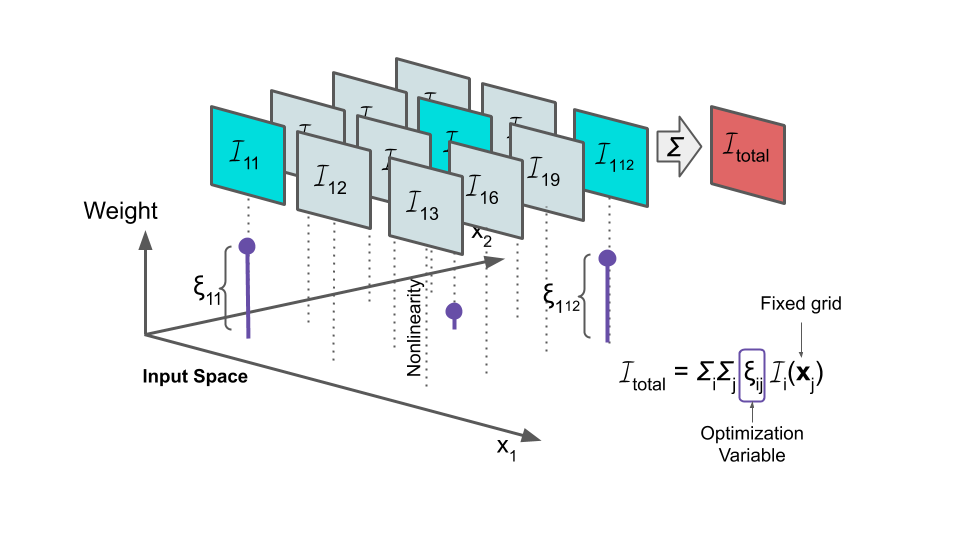
\includegraphics[scale=.4]{Images/discrete_graphic.png}
\caption{A depiction of NLOED design optimization problem structure with two discretized  inputs and a single observation variable.}
\label{fig:discrete_opt}
\end{figure}

The input settings the user provides in \texttt{discrete\_inputs} and \texttt{continuous\_inputs} during instantiation of the \texttt{Design} object significantly influence the optimization problem's computational structure. For example when only discrete inputs are used, the candidate grid specified by the user effectively becomes the support points set $\bm{x}_j\in\mathcal{X}$. As these points are fixed at specific levels in the grid, the input points, $\bm{x}_j$, are not included as free optimization variables in the optimization problem. Instead, the weights, $\xi_{i,j}$, become the only optimization variables. This results in a large sparse convex optimization problem, because the individual FIMs, $\mathcal{I}_i(\bm{x}_j,\bar{\bm{\theta}})$, for each candidate grid point, $\bm{x}_j$, can be pre-computed numerically before calling the solver. However, the weights, $\xi_{i,j}$, then control the exact convex combination of these matrices that make up the total FIM. The optimal support points will be indicated by the non-zero replicate weights after optimization. Non-zero replicate weights also indicate which observation variables are to be measured. As each FIM is semi-positive definite, the overall problem is convex (at least for the default D-optimal objective) \cite{atkinson1992optimum}. However, the discrete handling of inputs requires the \texttt{Design} class to compute a FIM for every input grid point, which can be time consuming if there are many inputs and the grid points consist of all permutations of the candidate input levels. Figure \ref{fig:discrete_opt} visually depicts the optimization problem formulated with a discretized two dimensional input space and a single observation variable. This scenario would correspond to a \texttt{discrete\_inputs} dictionary structured as;
\begin{minted}[xleftmargin=\parindent,breaklines]{python}
discrete_dict = {'Inputs':['x1','x2'],
                 'Candidates':[[1,2,3],[1,2,3,4]]}
\end{minted}
In the figure, three levels of \texttt{x1} and four levels of \texttt{x2} are permuted to create a candidate grid over which the sampling weights serve as optimization variables. In summary, the optimizer has flexibility in assigning sampling weights and observation variables and will easily converge to a global optima, up to numerical precision, but the optimizer has no flexibility to adjust the grid of input points.

\begin{figure}[htb!]
\centering
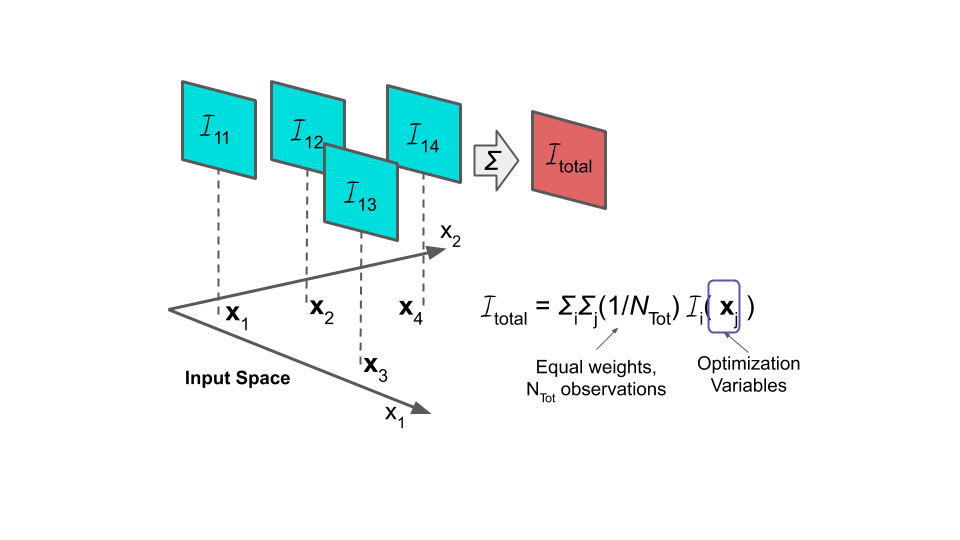
\includegraphics[scale=.4]{Images/locked_continuous_graphic.png}
\caption{A depiction of an NLOED design optimization problem structure with two continuously handled inputs and the \texttt{LockedWeights} constraint activated.}
\label{fig:continuous_opt_locked}
\end{figure}
A complimentary scenario to the discretized input grid optimization problem can be achieved, where the weights, $\xi_{i,j}$, are fixed and only the input points, $\bm{x}_j$, are optimized. This occurs when only continuous inputs are used, and the \texttt{LockWeights} option is set to \texttt{True}, so that each input point gets the same fixed weighting. In this case the user controls the number of unique support points, $N$, by specifying the size of the support set using the \texttt{Structure} field of the \texttt{continuous\_inputs} argument. Figure \ref{fig:continuous_opt_locked} depicts this optimization set up for a two input scenario. This would correspond to a \texttt{continuous\_inputs} argument structured as;
\begin{minted}[xleftmargin=\parindent,linenos,breaklines]{python}
continuous_dict = {'Inputs':['x1','x2'],
                   'Bounds':[(0,1),(0,1)],
                   'Structure':[['x1_lvl','x2_lvl1'],
                                ['x1_lv2','x2_lvl2'],
                                ['x1_lv3','x2_lvl3'],
                                ['x1_lv4','x2_lvl4']]}
\end{minted}
In the figure there are four support points free to vary within the bounded domain, each with a fixed identical sampling weight. Here, if the model is nonlinear in its parameters, then the input points, $\bm{x}_j$, are nonlinearly related to the optimization objective. This means the optimization becomes a fully nonlinear programming problem but it tends to be smaller as the number of optimization dimensions is the product of the input dimension size of $\bm{x}$ and the number of support points, $N$. Here the optimizer has great flexibility in moving the support points around the input space, but designs may be sensitive to the starting locations of the support points and no flexibility in re-weighting the support points is possible. In this scenario, the only way for the optimizer to replicate a support point is to locate two support points at an identical position, meaning the user will generally need to provide a large number of support points (potentially on the same order as their intended sample size) in order to understand the optimal replication structure. However, the resulting designs derived with locked weights are easily implemented exactly with small sample sizes. 

\begin{figure}[htb!]
\centering
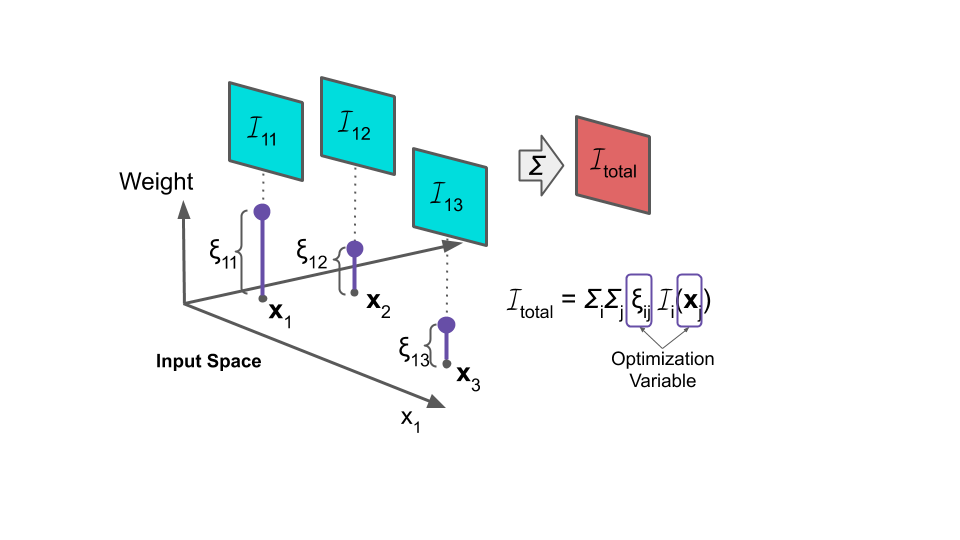
\includegraphics[scale=.4]{Images/continuous_graphic.png}
\caption{A depiction of NLOED design optimization problem structure with two continuously handled inputs, optimized sampling weights, and a single observation variable.}
\label{fig:continuous_opt}
\end{figure}
When continuous inputs are used in the default manner, without locked weights, both the weights, $\xi_{i,j}$, and the input points, $\bm{x}_j$, are treated as optimization variables. This scenario is depicted in Figure \ref{fig:continuous_opt} and would equate with a \texttt{continuous\_inputs} argument structured as:
\begin{minted}[xleftmargin=\parindent,linenos,breaklines]{python}
continuous_dict = {'Inputs':['x1','x2'],
                   'Bounds':[(0,1),(0,1)],
                   'Structure':[['x1_lvl','x2_lvl1'],
                                ['x1_lv2','x2_lvl2'],
                                ['x1_lv3','x2_lvl3']]}
\end{minted}
This setup gives the optimizer flexibility in both the location of the support points and in the distribution of samples amongst support points as both points and weights are optimization variables. In the figure there are three support points, each with its own sampling weight. The resulting problem is still highly nonlinear in the support points but the use of the weights means that user can allot less candidate support points and still discover the optimal replication structure. This can lead to a smaller optimization problem but the resulting design may be more suited to a large sample size for implementation. 

\begin{figure}[htb!]
\centering
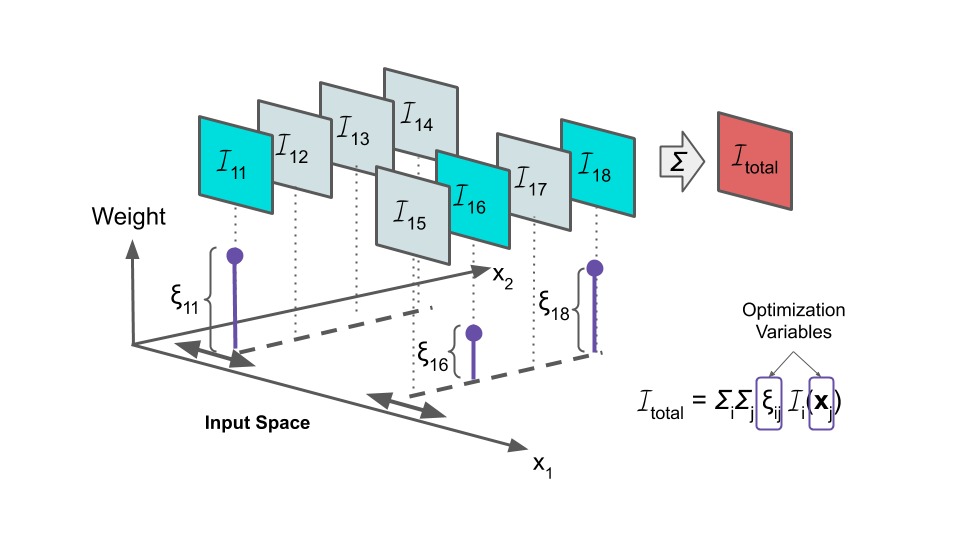
\includegraphics[scale=.4]{Images/mixed_graphic.png}
\caption{A depiction of NLOED's design optimization problem structure with the first input dimension handled continuously and the second input dimension handled discretely, and with a single observation variable.}
\label{fig:mixed_opt}
\end{figure}
Mixing continuous and discrete inputs can lead to complicated structures which are difficult to visualize. In the continuous subspace of the overall input space, a certain number of candidate support points are free to vary during optimization, as specified by the \texttt{Structure} key in the \texttt{continuous\_inputs} argument. (Recall these `points' are technically in a lower dimensional sub-space of the overall input space which consists of only the continuously assigned dimensions). Along the remaining discretely handled input dimensions, a candidate set of levels is available via the discrete grid. An example of this scenario is depicted in Figure \ref{fig:mixed_opt}. This scenario would correspond to the \texttt{discrete\_inputs} and \texttt{continuous\_inputs} arguments structured as;
\begin{minted}[xleftmargin=\parindent,linenos,breaklines]{python}
#discreet_inputs argument
discrete_dict ={'Inputs':['x2'],
                'Candidates':[[1,2,3,4]]}
#continuos_inputs argument
continuous_dict = {'Inputs':['x1'],
                   'Bounds':[(0,1)],
                   'Structure':[['x1_lvl1'],
                                ['x1_lvl2']]}
\end{minted}
Here two unique levels of input \texttt{x1} are available to the optimizer. At each of these two levels, in the second dimension, \texttt{x2}, a four level grid is available for selection via the sampling weights. The optimal set of support points that are selected is a function of the location of the continuous dimension points and which discrete grid locations receive non-zero weights. This type of problem formulation allows the user to accommodate specific experimental limitations, for example if \texttt{x2} can only be set to four discrete levels in the available equipment, and if \texttt{x1} can only be run with at most two unique levels in the given round of experimentation. The mixed formulation can also decrease the non-linearity of a problem, as the input dimensions that are handled continuously are the only ones that are fully nonlinear with respect to the objective. 


\begin{figure}[htb!]
\centering
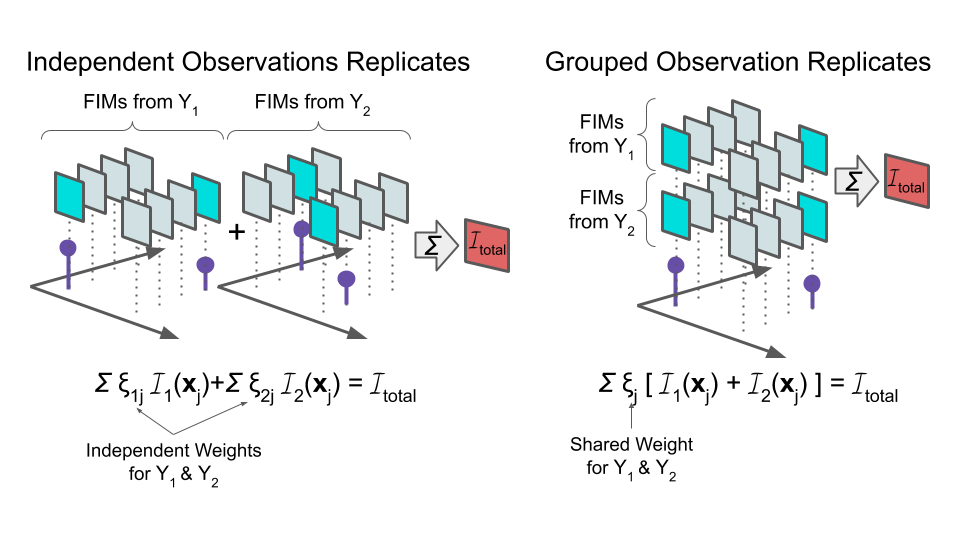
\includegraphics[scale=.4]{Images/obs_opt.png}
\caption{A depiction of NLOED's method for observation selection as part of its optimization structure. On the left, the default method is used, where observation variables \texttt{y1} and \texttt{y2} are each given a separate set of weights over the same input structure. On the right, the \texttt{observ\_struct} has specified that \texttt{y1} and \texttt{y2} must be observed together in any given input conditions.}
\label{fig:obs_opt}
\end{figure}
For models with multiple observation variables, output selection is performed in a similar manner to discrete input selection. Non-zero weights, $\xi_{i,j}$, are used to decide which outputs are measured. Figure \ref{fig:obs_opt} shows the default handling of multiple observation variables for a two input model on the left. In this case each of the outputs, \texttt{y1} and \texttt{y2}, has its own FIM with its own weight but they both share the same underlying input points, regardless of whether inputs are handled continuously, discretely, or in a mixed fashion. When the user groups outputs together using the \texttt{observ\_struct} argument, the FIMs are automatically summed within the group before they are weighted, implying that they are always observed as a group. This situation is shown on the right in Figure \ref{fig:obs_opt} for a two output model where both outputs, \texttt{y1} and \texttt{y2} have been grouped together.

Based on the provided inputs to \texttt{Design} constructor NLOED will implement the appropriate optimization scenario. Each scenario results in different symbolic structures, which are then passed to IPOPT. Some experimentation may be necessary with a given experimental design problem in order to find a structure which works well in IPOPT and satisfies experimental constraints. After optimization, the relaxed design is parsed from IPOPT's output and stored within the \texttt{Design} object. The user can then view the relaxed design with its continuous weights or generate an exact design using the objects user-callable functions described in the next section. While NLOED provides extensive flexibility in formulating the optimal design problem, not all experimental limitations can be implemented. In these scenarios, the optimal relaxed design can often provide qualitative information about which input conditions provide the most desirable information about the model parameters. The user can then use the \texttt{Model} class's \texttt{evaluate()} function and simulation tools to assess design modifications and find a reasonable design.

% Internal Workings
% \begin{itemize}
%   \item FIM is additive over observations, goal of optimizer is to choose optimal inputs and weights for best objective of the fim.
%   \item Discrete inputs are treated as options from a grid of candidates, optimizer chooses weighting
%   \item Continuous inputs, each row in archetype is a possible unique point in continuous subspace, each unique variable in row is a degree of freedom for that point
%   \item Example: mixed formulation, one discrete one cont.
%   \item Example: shared variable across columnbs in archetype 
%   \item prior info on parameter or multiple models just replicate computation
%   \item Design automatically sets up optimization problem and sovles relaxed version: end result is an unrounded design, given example.
% \end{itemize}

%As all observations in NLOED are assumed to be independent, the computation of the Fisher information matrix is additive over all candidate observations. 

% FIM is additive, we solve relaxed problem so optimize weights,

% Mulitple observation types are each given their own weights, hence how observation selection is implemented.

% user controls this primarily in specifying which inputs are handled continously and which are handled discretly

% This in turn influences the convexity of the problem; whether it is convex or fully nonlinear.

% This also influences the resolution or discretness of the optimal solution in the control space i.e. if input is treated discretely the optimal solution can only contain certain levels of the input (this is good if those levels are real, but an approximation with fixed resolution if the input is actually continuous and it has been discretized as an approximation.

% Specifying input as discrete implies lots of upfront comp of FIM's at each discete point but optimization is done over weights for each pre-computed fim, is fairly easy and convex. Better for...
% (Discrete input essential breaks the problem up and treats every possible input and observation pair like a separate possible obseravtion variable that can or cannot be included in the final design)

% If inputs are treated as continous, the individual points in the input space are optimized, this is much more nonlinear and requires the user to specify the number of unique points to be considered. Less upfront computation but more required at each iteration, better for...

% Given some objective $D(.)$
% \begin{align}
% \begin{aligned}
% \mathcal{I}_{Tot} = \sum_i^M \beta_i \mathcal{I}_i(\bm{x_i},y_i)
% \end{aligned}
% \label{eq:nloed_objective}
% \end{align}


\subsection{User-callable \texttt{Design} Functions}

%\textbf{This subsection discusses what functions are available from a Design class object after it is created. Users can round the relaxed design into an exact design. We can explain the rounding procedure. The user can also do some power analysis and post-hoc optimization via two other functions that will be described.}

Once the user has instantiated a \texttt{Design} object instance, they can use the object to examine the optimal design structure and to generate exact designs that can be implemented in practice or be simulated by the \texttt{Model} class. The user can perform these actions by calling functions available within the \texttt{Design} class object. Here we explain the calling procedure for the available functions and discuss some planned extensions. 

\paragraph{The \texttt{relaxed()} function}

The \texttt{relaxed()} function can be used to return the relaxed optimal design as a dataframe. Relaxed designs resemble exact designs however instead of a \texttt{Replicates} column containing the integer count of replicate allocations, $\beta_{i,j}$, they have a \texttt{Weight} column that contains the real valued weights, $\xi_{i,j}$. The sum of the \texttt{Weight} column values will be one, up to the numerical precision of the optimization algorithm. 
The \texttt{relaxed()} function does not accept any input arguments. An example call is shown in Listing \ref{lst:relaxed_func_exmp}.
\begin{listing}[H]
\begin{minted}[xleftmargin=\parindent,linenos,breaklines]{python}
#extract the relaxed design from the design object
relaxed_design = design_object.relaxed()
#print the relaxed design
print(relaxed_design)
\end{minted}
\caption{An example call to the \texttt{Design} class's \texttt{relaxed()} function.}
\label{lst:relaxed_func_exmp}
\end{listing}
\noindent Line 2 returns the relaxed design dataframe and in line 4 the dataframe is printed to the output. An example of a relaxed design that has been printed is shown in Figure \ref{fig:relaxed_return}.
\begin{figure}[htb!]
\centering
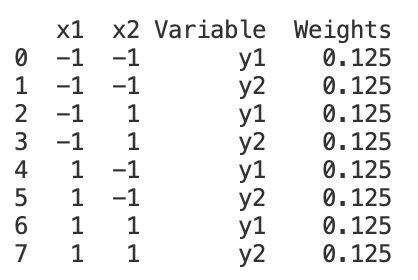
\includegraphics[scale=.7]{Images/relaxed_example.png}
\caption{An example of a dataframe containing an relaxed design returned by the \texttt{relaxed()} fucntion.}
\label{fig:relaxed_return}
\end{figure}
Here we can see that there are only four unique support points, with different input values of \texttt{x1} and \texttt{x2}, each with even weighting across both observation variables \texttt{y1} and \texttt{y2}. This result is typical for linear models with normal errors and symmetric bounds on the input domain. Returning the relaxed design is not generally necessary but as the relaxed design is used to generate all exact designs via rounding, it can be useful for visualizing the underlying relaxed structure. In addition, depending on how the design optimization problem was structured, the relaxed design may be guaranteed to satisfy certain equivalence theorems \cite{atkinson1992optimum}, and thus can be used to verify a global optima has been achieved. This will only work in special cases, for more information the user may refer to \cite{atkinson1992optimum}.

\paragraph{The \texttt{round()} function}

In order to create an exact design with a finite sample size, $N_{Tot}$, the user must discretize the exact design in some manner, converting real-valued weights, $\xi_{i,j}$ to integer valued allocations, $\beta_{i,j}$, so that $N_{Tot}=\sum_j^N\sum_i^M \beta_{i,j}$. There are a number of rounding methods available, each with various trade-offs \cite{pukelsheim1992efficient,wilhelm1996obtain,imhof2001efficiencies}. The \texttt{round()} function implements the Adam's apportionment rounding procedure as a default method for performing this task. Adam's apportionment has been noted in previous works as having a number of ideal properties for rounding experimental designs \cite{pukelsheim1992efficient,wilhelm1996obtain,imhof2001efficiencies}. The general call structure for the \texttt{round()} function is;
\begin{minted}[xleftmargin=\parindent,breaklines]{python}
round(sample_size, options={})
\end{minted}
The \texttt{sample\_size} argument accepts the desired number of sample size for the experiment. The \texttt{options} argument is optional and can be used to override the default behaviour of the rounding algorithm. An example call to the \texttt{round()} function is shown in Listing \ref{lst:round_func_exmp}.
\begin{listing}[H]
\begin{minted}[xleftmargin=\parindent,linenos,breaklines]{python}
#set the sample size
sample_size = 10
#generate the rounded design
exact_design = design_object.round(sample_size)
#print the resulting exact design
print(exact_design)
\end{minted}
\caption{An example call to the \texttt{Design} class's \texttt{round()} function.}
\label{lst:round_func_exmp}
\end{listing}
\noindent In line 2, the sample size, $N_{Tot}$, is set to 10, and in line 4 the exact design is generated with a call to the \texttt{round()} function of the \texttt{design\_object}. In line 6 the exact design is printed to the console output. An example of a exact design returned by the  \texttt{round()} function for the relaxed design shown in Figure \ref{fig:relaxed_return} is shown in Figure \ref{fig:round_return}.
\begin{figure}[htb!]
\centering
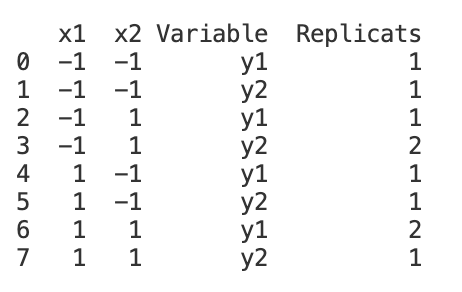
\includegraphics[scale=.7]{Images/rounded_example.png}
\caption{An example of an exact design dataframe returned by the \texttt{round()} function.}
\label{fig:round_return}
\end{figure}
The \texttt{round()} function here is called with a sample size of 10, however, the relaxed design has 8 unique input-observation pairs, each with equal weighting. As an equal weighting of 8 points is not achievable with 10 observations, the rounding procedure will allocate these additional points randomly. As in the above case Adam's method does not always yield a unique apportionment, in which case currently a random selection is made. In future versions of the package the \texttt{rounding()} function will be extended to allow more rounding methods as well as further analysis in cases where non-unique rounding occurs. %In future versions, the number of rounding methods will be extended, along with options to return the set of designs generated by a rounding method that terminates with a non-unique design. Tools to rank and quantify the various designs according to their loss in optimality compared to the relaxed design will also be included. 

\paragraph{The \texttt{power()} function}

Often the user's ultimate goal is to constrain parameter values within reasonable confidence bounds of a prescribed width. Experimental equipment or cost may place some upper bound on the sample size in a given experiment, and in cases where this is quite restrictive the user will use the maximum sample size as the input for the \texttt{round()} function. If the design achieves the desired accuracy than the task is achieved, and if not the experimenter may be forced to iterate over multiple rounds of experimentation.

However, in some cases there may not be a restrictive upper bound on the sample size, but rather observations may be costly in either time or resources and the user may prefer smaller sample sizes but has no firm upper limit. In this context the user needs a method to examine trade-offs in sample size and confidence interval width across a range of feasible sample sizes. This type of analysis is similar to \textit{power analysis} done for traditional regression models in empirical studies for social and medical sciences \cite{cohen2013statistical}. Power analysis can demonstrate how confidence intervals or other diagnostic metrics converge as the sample size increases.

The \texttt{power()} function is nor currently implemented but its intended role is to allow the user explore rounding of the optimal relaxed design for multiple sample sizes within a range. This process will allow the user to understand performance trade-offs across this range for the given design and to determine at what sample size threshold certain accuracy objectives are expected to be achieved. It is important to note that the same underlying relaxed design is used for each sample size to generate an exact design, however the exact designs will differ in replicate allocation. As the sample size increases the exact design can better approximate the optimal weights in the relaxed design. This generally results in a monotonic increase in performance for exact designs created with larger sample sizes; a larger sample size is almost always better. However, for some relaxed designs, certain integer sample sizes more accurately approximate the relaxed weights than other nearby, even larger, sample sizes. The larger sample sizes will always perform better, but the gains may be marginal relative to the cost for the experimenter. The \texttt{power()} function will provide graphical and quantitative methods to assess these trade-offs.

% can add citation here for certain type of diagnostic curve

%For example in an optimal relaxed design with three evenly weighted support points, a sample size of three will perfectly implement the relaxed design, with one sample for each support. If the user then tries to use a sample size of four, the resulting exact design will be better but only marginally so because the exact design samples are not allocated near the optimal weighting. If the user increases by another two, to have a sample size of six, the exact design will again replicate the relaxed design perfectly. Most of the gains in increasing the sample size from three to six are attained in the jump from 5 to 6. This type of analysis can be useful in deciding a good trade-off between sample size cost and design performance.
% User callable/ output
% \begin{itemize}
%     \item Print (relaxed design)
%   \item Round
%   \item Power (mention)
%   \item Optimize (mention)
% \end{itemize}

%Ds optimal design for model selection

% [In EXAMPLES?] ambiguity about certain inputs/conditions e.g. time/space can be treated as input or as diff observations, redundant somewhat for static models, but important for models that require numerical simulation. Always relevant for numerics, ie implies different things to be optimized in conjunction with discrete/continuous inputs.

\section{Examples}\label{package_examples}

In this section, we give a description of the package workflow using specific models. These examples include code snippets and sample output, and specifically focus on how models are encoded in CasADi's symbolics, and how the experimental constraints are passed to the \texttt{Design} class. These example, among other, will serve as prototypes for first-time users in the package documentation so that those new to the package have several working examples to start from and modify when they seek to implement their own projects.

%\textbf{This section is all about specific model examples and generating designs for them. We have already introduce all the different lines of code used here so most of it is about 1) setting the model up in Casadi, and 2) linking various parts of the Model and Design class together in a workflow. }

\subsection{Optimal Design for Static Models}

%\textbf{I want to start with a simple one-input, one-output steady state model, probably a Hill function. Then if there is time/space do a multi-input, multi-output steady state model with two error distributions (i.e. normal and Poisson). Most of this will be blocks of code with explaining text in between. If there is time I'll include code for plotting the design and data/predictions.}
%\paragraph{Optogenetic Dose-response Curve}
Here we begin by describing the NLOED package applied to a static model; one that does not require any numerical integration and therefore does not involve ODEs. As a first example we begin with a simple optogenetic dose response curve. Recall from previous chapters that an optogenetic system is one where gene expression can be activated by a the light intensity of a specific color. Here a Hill function is used to describe the expression of GFP as a function of the light intensity such that
\begin{align}
\textit{GFP}=\alpha_0+\alpha \frac{\textit{Light}^n}{K^n+\textit{Light}^n}.
\end{align}
Here $\alpha_0$, $\alpha$, $K$ and $n$ are the parameters of interest, \textit{Light} is the single experimental input and \textit{GFP} is the observed expression of GFP and the single model observable. We assume some past experimental data has been collected for this model but that the user wishes to improve the accuracy of the confidence intervals as efficiently as possible. We assume the user is also confident enough to assert that the distribution of the GFP expression level is normally distributed with a standard deviation of about 5\% of the mean expression level.

The user begins by starting their preferred Python interface and importing the required packages. Listing \ref{lst:ss_lst0} shows the the required commands in lines 1-6.
\begin{listing}[H]
\begin{minted}[xleftmargin=\parindent,linenos,breaklines]{python}
import numpy as np
import pandas as pd
import casadi as cs
import matplotlib.pyplot as plt
from nloed import Model
from nloed import Design
\end{minted}
\caption{Import statements for using the NLOED package, including the \texttt{Model} and \texttt{Design} class as well as other common Python numerical libraries.}
\label{lst:ss_lst0}
\end{listing}
\noindent Next in Listing \ref{lst:ss_lst1}, the user creates CasADi symbols for the input and parameters. This occurs in lines 8 and 9, note that the names here can be arbitrary. These lines make use of CasADi's \texttt{cs.SX.sym()} function to create two symbol vectors. The call to \texttt{cs.SX.sym()} for creating the experimental input has a single dimension (second argument omitted). The second call to \texttt{cs.SX.sym()} for the parameters has four dimensions, one for each parameter of interest. In lines 11-14 we define the named parameters used in the model definition to be the exponentiated values of the parameters in the \texttt{parameters} vector. This is a log transformation and it ensures that the named parameter values are always positive.  This type of transformation is an important consideration when working with bounded parameter ranges. Asymptotic expressions for parameter variability, like the Fisher information matrix, are more cumbersome to compute for bounded parameter domains and thus NLOED assumes the user either transforms their parameters to avoid the need for bounding or that the feasible parameter range is so distant from the bounds they can safely be ignored during model calibration. Here we have chosen a simple transformation to avoid the need for bounds. A log transformation can also sometimes improve the numerical performance of the design and fitting algorithms. The named parameters are given for clarity but the user could choose to perform the transformation and model definition together for brevity. 
\begin{listing}[H]
\begin{minted}[xleftmargin=\parindent,linenos,breaklines,firstnumber=last]{python}
#define input and parameter symbols
inputs = cs.SX.sym('inputs')
parameters = cs.SX.sym('parameters',4)
#log-transormation of the parameters
alpha0 = cs.exp(parameters[0]) 
alpha = cs.exp(parameters[1]) 
n = cs.exp(parameters[2]) 
K = cs.exp(parameters[3]) 
#define the deterministic model for the GFP mean
gfp_mean = alpha0 + alpha*inputs**n/(K**n+inputs**n)
#assume some hetroskedasticity, std_dev 5% of mean expression level
gfp_var = (0.05*gfp_mean)**2
#link the deterministic model to the sampling statistics (here normal mean and variance)
gfp_stats = cs.vertcat(gfp_mean, gfp_var)
#create a casadi function mapping input and parameters to sampling statistics (mean and var)
gfp_model = cs.Function('GFP',[inputs,parameters],[gfp_stats])
\end{minted}
\caption{An example of building a CasADi function for the deterministic component of the optogenetic dose-response model, before making a call to the \texttt{Model} constructor.}
\label{lst:ss_lst1}
\end{listing}
\noindent In line 16, the mean GFP response, \texttt{gfp\_mean}, is defined in terms of the named parameters and the input. In line 18 the variance of the GFP observations, \texttt{gfp\_var}, is defined to be the square of 5\% of the mean GFP expression. In line 20 the mean and variance are concatenated into a single vector, this is mainly done for clarity and it could be merged into the following line. In line 22, a CasADi function, \texttt{gfp\_model}, is defined using CasADi's \texttt{cs.Function()} constructor, this function maps the input and parameters to the GFP sampling statistics. Up to this point the naming of all variables and CasADi symbols was arbitrary, however now the string passed to the \texttt{Function()} constructor (in this case `\texttt{GFP}') will become the name of the observation variable within the NLOED Model. 

Having created a CasADi symbol for the GFP observation variable, the user can now construct an NLOED \texttt{Model} instance. Listing \ref{lst:ss_lst2} demonstrates this process. In line 24, the \texttt{gfp\_model} function is tupled with the label \texttt{Normal} indicating that it describes the sampling statistics of a normal random variable. This tuple is placed in the list \texttt{observ\_list}. If the model had more observation variables they would also be entered as tuples in the same list, however as the current model has a single observation dimension, the list is a singleton. In lines 26 and 28, names for the input and parameters are given in vectors \texttt{input\_names} and \texttt{parameter\_names} respectively. In line 30, the NLOED model constructor is called with the three preceding lists as arguments. The \texttt{model\_object} variable now contains an instance of an NLOED \texttt{Model} class encoding the dose-response model.
\begin{listing}[H]
\begin{minted}[xleftmargin=\parindent,linenos,breaklines,firstnumber=last]{python}
# create observation list, add model function with 'Normal' label as tuple 
observ_list = [(gfp_model,'Normal')]
#create names for inputs
input_names = ['Light']
#create names for parameters
parameter_names = ['log_Alpha0','log_Alpha','log_n','log_K']
#instantiate nloed model class
model_object = Model(observ_list,input_names,parameter_names)
\end{minted}
\caption{Code showing the instantiation of an NLOED \texttt{Model} instance for the optogenetic dose-response model.}
\label{lst:ss_lst2}
\end{listing}

We assume the user has some preliminary data describing the GFP-intensity does response relationship, shown as a dataframne in Figure \ref{fig:ss_init_data}. Here there are triplicate observations at four different light intensities 0.1, 3.0, 6.0 and 10.0. (We use this dataset as a stand in for real experimental data, however it was actually generated using the \texttt{sample()} function from the \texttt{Model} class using parameter vector $[2,10,2,3]$ which we pretend we do not know for this analysis.) We assume this initial data is contained in the dataframe \texttt{init\_data}.
\begin{figure}[htb!]
\centering
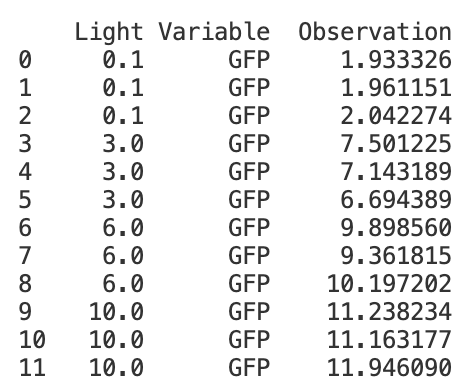
\includegraphics[scale=.7]{Images/ss_init_data.png}
\caption{An example dataset for the optogenetic dose-response model, with triplicate measurements of GFP taken at four different light levels.}
\label{fig:ss_init_data}
\end{figure}
The user can perform an initial fit to the preliminary data using the \texttt{Model} class's \texttt{fit()} function. Listing \ref{lst:ss_lst3} demonstrates this procedure. In lines 32-33, fit options are set, specifying a range for the parameter pre-search. Here a $7^4$ element grid of initial parameters vectors are distributed over the region in parameter space specified by the bound tuple list. The pre-fitting search evaluates each of these points for a good candidate starting point for the maximum likelihood optimization. Using the pre-search is ideal when an initial parameter guess is not possible, as in this case. In line 35, the \texttt{fit()} function of the \texttt{model\_object} is used to fit the model to the data in \texttt{init\_data}. In line 37, we extract the fit parameter values into a Numpy array, numerically they correspond to $[1.87,12.20,1.31,3.72]$
\begin{listing}[H]
\begin{minted}[xleftmargin=\parindent,linenos,breaklines,firstnumber=last]{python}
#set options to use a simple initial search
fit_options={'InitParamBounds':[(-1,2),(1,3),(-1,2),(-1,2)],
             'InitSearchNumber':7}
#fit the model to the initial data
fit_info = model_object.fit(init_data, options=fit_options)
#extract the parameter values
fit_params = fit_info['Estimate'].to_numpy().flatten()
\end{minted}
\caption{Code showing the optogenetic dose-response being fit to an initial dataset using the \texttt{fit()} function.}
\label{lst:ss_lst3}
\end{listing}
To get a sense for the initial uncertainty in the parameter values we can use the \texttt{evaluate()} function in the \texttt{Model} class to generate the asymptotic covariance matrix for the inital data's design. Listing \ref{lst:ss_lst4} shows this process, in line 39-41 we enter the design information for the initial dataset. In lines 43-44, the covariance matrix is requested and the method for computing the matrix is specified in the options dictionary. In line 46 the \texttt{evaluate()} function is called from the \texttt{model\_object}, using the fit parameters values stored in the \texttt{fit\_params} array.  In lines 48-49, we compute the approximate Wald confidence interval bounds.
\begin{listing}[H]
\begin{minted}[xleftmargin=\parindent,linenos,breaklines,firstnumber=last]{python}
# enter the initial design information
init_design = pd.DataFrame({'Light':[.1,3,6,10],
                            'Variable':['GFP']*4 ,
                            'replicates':[3]*4})
#request the asymptotic covariance matrix
eval_options={'Method':'Asymptotic',
              'Covariance':True}
# call evaluate() to compute the asymptotic covariance
asymptotic_covariance = model_object.evaluate(init_design,fit_params,eval_options)
#compute the asymptotic upper and lower 95\% bounds
asymptotic_lower_bound = fit_params - 2*np.sqrt(np.diag(asymptotic_covariance))
asymptotic_upper_bound = fit_params + 2*np.sqrt(np.diag(asymptotic_covariance))
\end{minted}
\caption{Code showing the use of the \texttt{evaluate()} function to generate the asymptotic covariance matrix and Wald confidence interval bounds for the initial dataset.}
\label{lst:ss_lst4}
\end{listing}
The resulting confidence intervals are printed in Figure \ref{fig:ss_init_bnds}. As we know the `true' values from which the data was generated, we can see the intervals contain the data-generating parameter vector, however the point estimate could certainly be improved. The user, who only has experimental data, would not know the true error, however the width of the confidence intervals is an indicator that accuracy could be improved.
\begin{figure}[htb!]
\centering
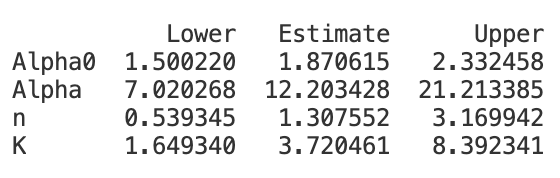
\includegraphics[scale=.7]{Images/ss_init_bnds.png}
\caption{A print out of the returned 95\% Wald confidence bounds for the optogenetic dose-response model fit to the initial dataset.}
\label{fig:ss_init_bnds}
\end{figure}

The parameter uncertainty captured in the asymptotic covariance matrix can also be used to approximate how much prediction uncertainty there is conditioned on our uncertainty in the parameter values and our knowledge of the sampling statistics. Listing \ref{lst:ss_lst5} demonstrates how this is done using the \texttt{Model} class's \texttt{predict()} function; in line 51 the asymptotic covariance matrix is converted to a Numpy matrix. In line 53-54, we specify the model predictions that are desired for plotting. We request 100 light levels linearly spaced between 0.1 and 10, all of which are of the \texttt{GFP} observation variable. In lines 56-57, we specify that the \texttt{predict()} function should return both prediction and observation intervals in the options dictionary. In lines 59-62, the \texttt{predict()} function is called at the estimated parameter values.
\begin{listing}[H]
\begin{minted}[xleftmargin=\parindent,linenos,breaklines,firstnumber=last]{python}
#convert the covariance matrix to a Numpy array
covariance_matrix = asymptotic_covariance.to_numpy()
#select prediction intputs
prediction_inputs = pd.DataFrame({'Light':np.linspace(0.1,10,100),
                                  'Variable':['GFP']*100})
#request prediction and observation intervals
prediction_options = {'PredictionInterval':True,
                      'ObservationInterval':True}
#call predict()
predictions = model_object.predict(prediction_inputs,
                                   fit_params,
                                   covariance_matrix = covariance_matrix,
                                   options=prediction_options)
\end{minted}
\caption{Code showing the use of the predict function to generate the mean dose response given the parameter estimates, along with 95\% prediction and observation intervals using the asymptotic covariance matrix.}
\label{lst:ss_lst5}
\end{listing}
The result of the call to the \texttt{predict()} function is shown in Figure \ref{fig:ss_init_pred}. Here the predicted mean GFP level at the parameter estimates is shown in dark blue. The blue region surrounding the prediction indicates the asymptotic approximation of the 95\% confidence region for the mean GFP response given the parameter uncertainty. Here we can see that a large amount of uncertainty regarding model behaviour is concentrated in the light intensity ranges between 0 and 2. This indicates that the constraints the initial data places on the model leaves this region subject to great uncertainty and future experiments will ideally provide better constraints on this region. The orange region indicates the approximate 95\% bounds on the data, meaning that given uncertainty in both the parameters and sampling error we would expect, approximately, that 95\% of the data would fall in this region.
\begin{figure}[htb!]
\centering
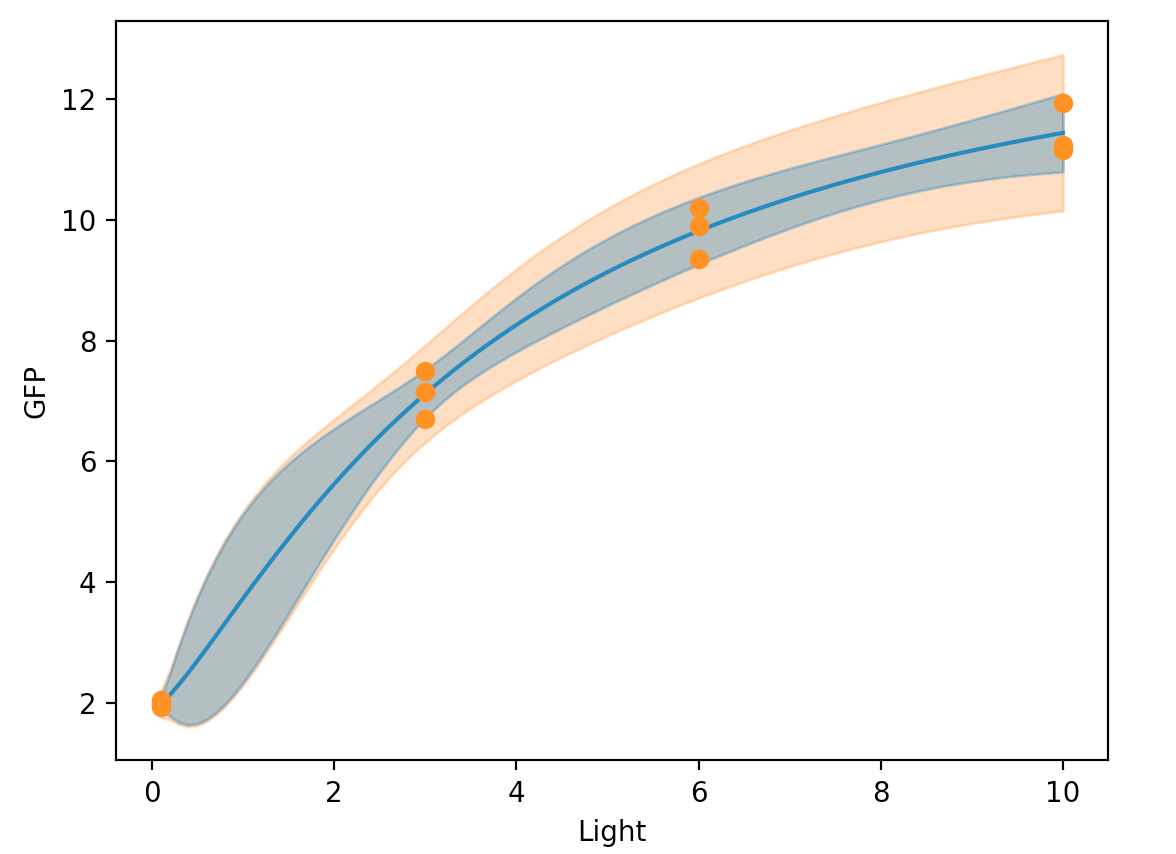
\includegraphics[scale=.7]{Images/ss_init_pred.png}
\caption{Mean GFP response (blue line), 95\% prediction intervals (blue region) and 95\% observation intervals (orange region) for the optogenetic model after fitting to the initial dataset (orange dots).}
\label{fig:ss_init_pred}
\end{figure}


Given the analysis of the initial uncertainty in the parameter estimates and the prediction accuracy, the user will likely wish to improve model fit in the next round of planned experiments. Listing \ref{lst:ss_lst6} shows the process of defining a \texttt{Design} class instance to generate an optimal design for the next set of measurements. Here we choose to treat the light level as continuous as the intensity can be varied to a fine degree in the lab relative the model's sensitivity over that range. In lines 64-67, we initialize the continuous input options so that we consider four unique light levels, just like in the initial experiment, that are free to be set between the light intensity bounds of 0.1 to 10. We assume these bounds are the limits of the experimental equipment. In line 68, we specify the initial design as having a weight of 0.33. Given the initial dataset contained 12 measurements, this assumes the next round of experiments will make approximately 24 GFP measurements. Here \texttt{init\_design} contains the design for the initial dataset; it is a dataframe similar to the \texttt{init\_data} but specifying replicate counts instead of observations. In lines 70-72, the \texttt{Design} class constructor is called and an instance is returned named \texttt{design\_object}. 
\begin{listing}[H]
\begin{minted}[xleftmargin=\parindent,linenos,breaklines,firstnumber=last]{python}
#set 'Light' as a continuous input with 4 unique levels
continuous_inputs={'Inputs':['Light'],
                   'Bounds':[(.01,10)],
                   'Structure':[['x1'],['x2'],['x3'],['x4']]}
#set fixed design dictionary with init design and weight
fixed_dict ={'Weight':0.33,'Design':init_design}
# generate the optimal design object
design_object = Design(model_object,fit_params,'D',
                       fixed_design = fixed_dict,
                       continuous_inputs = continuous_inputs)
#extract the relaxed design structure
relaxed_design = design_object.relaxed()
#set the sample size to 30
sample_size = 24
#generate a rounded exact design 
exact_design = design_object.round(sample_size)
\end{minted}
\caption{Code showing the process of creating an optimized \texttt{Design} object for the optogenetic dose-response model. Here the relaxed design is also returned and an exact design is generated through rounding.}
\label{lst:ss_lst6}
\end{listing}
\noindent In line 76, we use the \texttt{relaxed()} function of the \texttt{Design} class to return the relaxed design. This dataframe is shown in Figure \ref{fig:ss_relaxed}. We can see that the optimal relaxed design consists of four unique light levels with asymmetric weights. It is not surprising that approximately 40\% of the sampling weight is concentrated at a light level of 0.66, an input that is within the uncertainty bulge in the prediction interval plot in Figure \ref{fig:ss_init_pred}.
\begin{figure}[htb!]
\centering
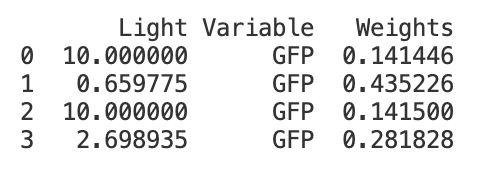
\includegraphics[scale=.7]{Images/ss_relaxed.png}
\caption{Output of the relaxed design from the \texttt{relaxed()} function for the optogenetic dose-response model.}
\label{fig:ss_relaxed}
\end{figure}
In line 76 of Listing \ref{lst:ss_lst6}, we set the sample size to 24 and in line 78 the \texttt{round()} function of the \texttt{Design} class is used to generate an exact design. The exact design is shown in Figure \ref{fig:ss_exact}. 
\begin{figure}[htb!]
\centering
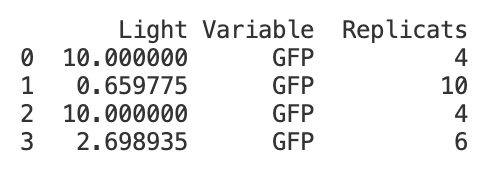
\includegraphics[scale=.7]{Images/ss_exact.png}
\caption{Output showing the exact design for the optogenetic dose-response model generated from the \texttt{round()} function.}
\label{fig:ss_exact}
\end{figure}

Before implementing the exact design in the laboratory it is useful to assess what the optimal designs expected utility is when combined with the initial data. This can be done by concatenating the initial and optimal design dataframes as follows:
\begin{minted}[xleftmargin=\parindent,breaklines,firstnumber=last]{python}
combined_design = pd.concat([init_design, exact_design], ignore_index=True)
\end{minted}
The \texttt{combined\_design} dataframe can then analysed using the same code shown in Listings \ref{lst:ss_lst4} and \ref{lst:ss_lst5}. The resulting expected asymptotic confidence intervals for the combined data are shown in Figure \ref{fig:ss_fim_bnds}. Here we see that the intervals are expect to shrink considerably after adding the optimal data. 
\begin{figure}[htb!]
\centering
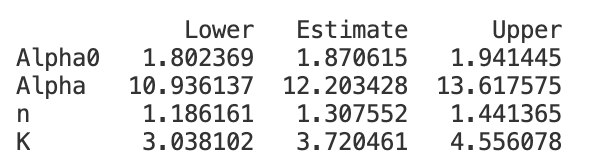
\includegraphics[scale=.7]{Images/ss_fim_bnds_update.png}
\caption{Expected 95\% confidence intervals for the optogenetic dose-response model parameters computed using the \texttt{evaluate()} function after combining the initial and optimal designs. }
\label{fig:ss_fim_bnds_update}
\end{figure}
In addition, we can generate prediction and observation intervals with the expected asymptotic convariance matrix of the combined data in a similar manner to that used for the initial data.  The prediction intervals are also expected to shrink considerably after implementing the optimal design, as shown in Figure \ref{fig:ss_pred_update}
\begin{figure}[htb!]
\centering
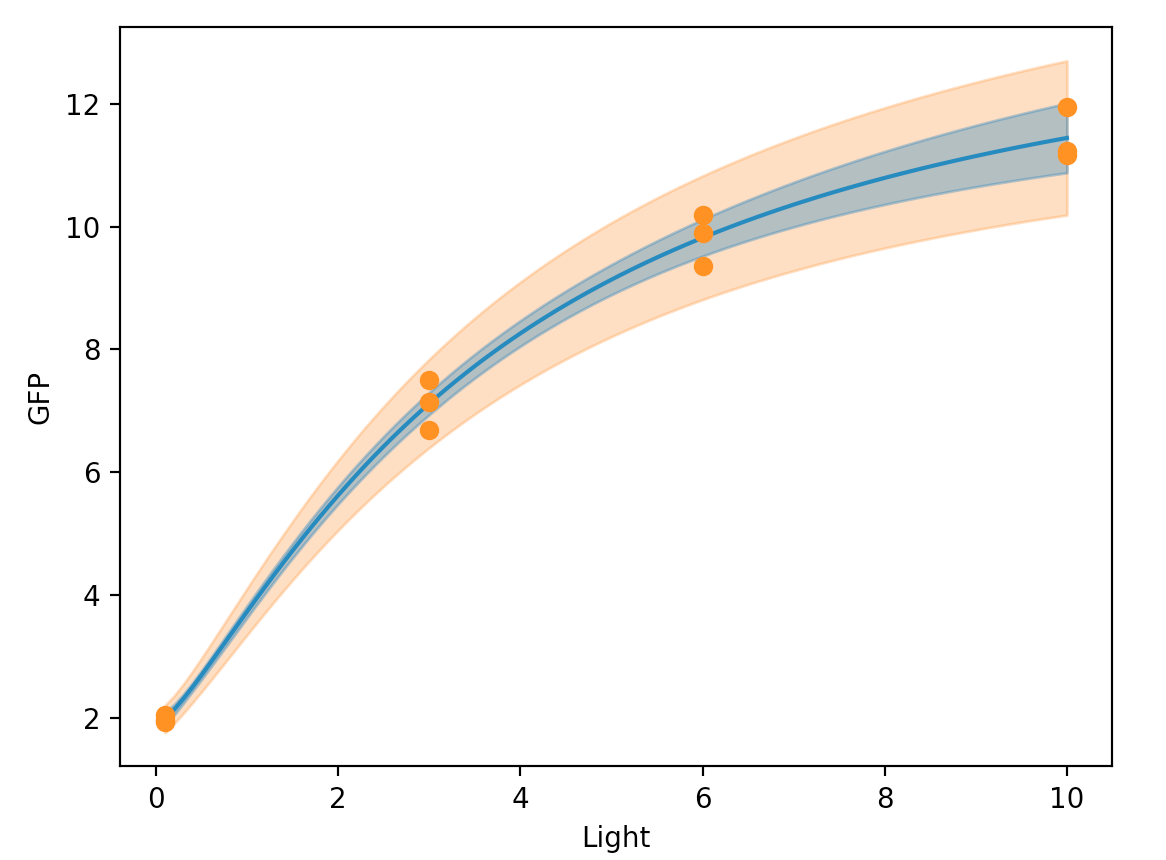
\includegraphics[scale=.7]{Images/ss_pred_update.png}
\caption{A plot of the 95\% prediction and observation intervals under the asymptotic covariance matrix from the combined initial and optimal designs, computed with the \texttt{predict()} function.}
\label{fig:ss_pred_update}
\end{figure}

At this point the user would perform the optimal experiment and return with the new data. Assuming the user has imported these observations into a dataframe named \texttt{optimal\_data}, a combined dataset can be generated and the model can be re-fit. This process is shown in Listing \ref{lst:ss_lst7}. In line 81 the initial dataset and optimal dataset are combined into a single dataframe. In line 83, an options dictionary is created to request the likelihood contours from the fitting algorithm so that we can visualize the likelihood profiles and 2D contour projections as diagnostics for the final fit.  In line 85, the \texttt{fit()} is called to fit the model to the combined dataset. In line 87, the fit parameters are extracted from the from the returned dataframe into a Numpy array. The resulting parameter vector is $[1.96, 10.04, 1.93, 2.98]$.
\begin{listing}[H]
\begin{minted}[xleftmargin=\parindent,linenos,breaklines,firstnumber=last]{python}
#combine the initial and optimal design
combined_data = pd.concat([init_data, optimal_data], ignore_index=True)
#request contours and use a simple initial search
fit_options={'Confidence':'Contours'}
#fit the model to the initial data
fit_info = model_object.fit(combined_data,start_param = fit_params, options=fit_options)
#extract the parameter values
fit_params = fit_info['Estimate'].to_numpy().flatten()
\end{minted}
\caption{Code showing the concatination of the initial and optimal datasets, and their combined fitting to the optogenetic dose-response model. Fitting is called with a request for likelihood confidence contours for diagnostic purposes.}
\label{lst:ss_lst7}
\end{listing}
\noindent During fitting the \texttt{fit()} function generates the likelihood profiles, trace projections and contour projections shown in Figure \ref{fig:ss_contours}. Here the profiles (blue curves along the diagonal plots) are nearly parabolic and the profile traces make `X' shapes (blue and orange curves in the lower triangular plots). Some irregularity is detectable in the eccentricity of the 95\% contour traces which are not quite elliptical, and some curvature can be seen in the profile traces which deviate from linearity at their endpoints. Overall this diagnostics looks reasonable and the data appears to constrain the model parameters well suggesting the approximations being used to assess parameter accuracy are themselves accurate. 
\begin{figure}[htb!]
\centering
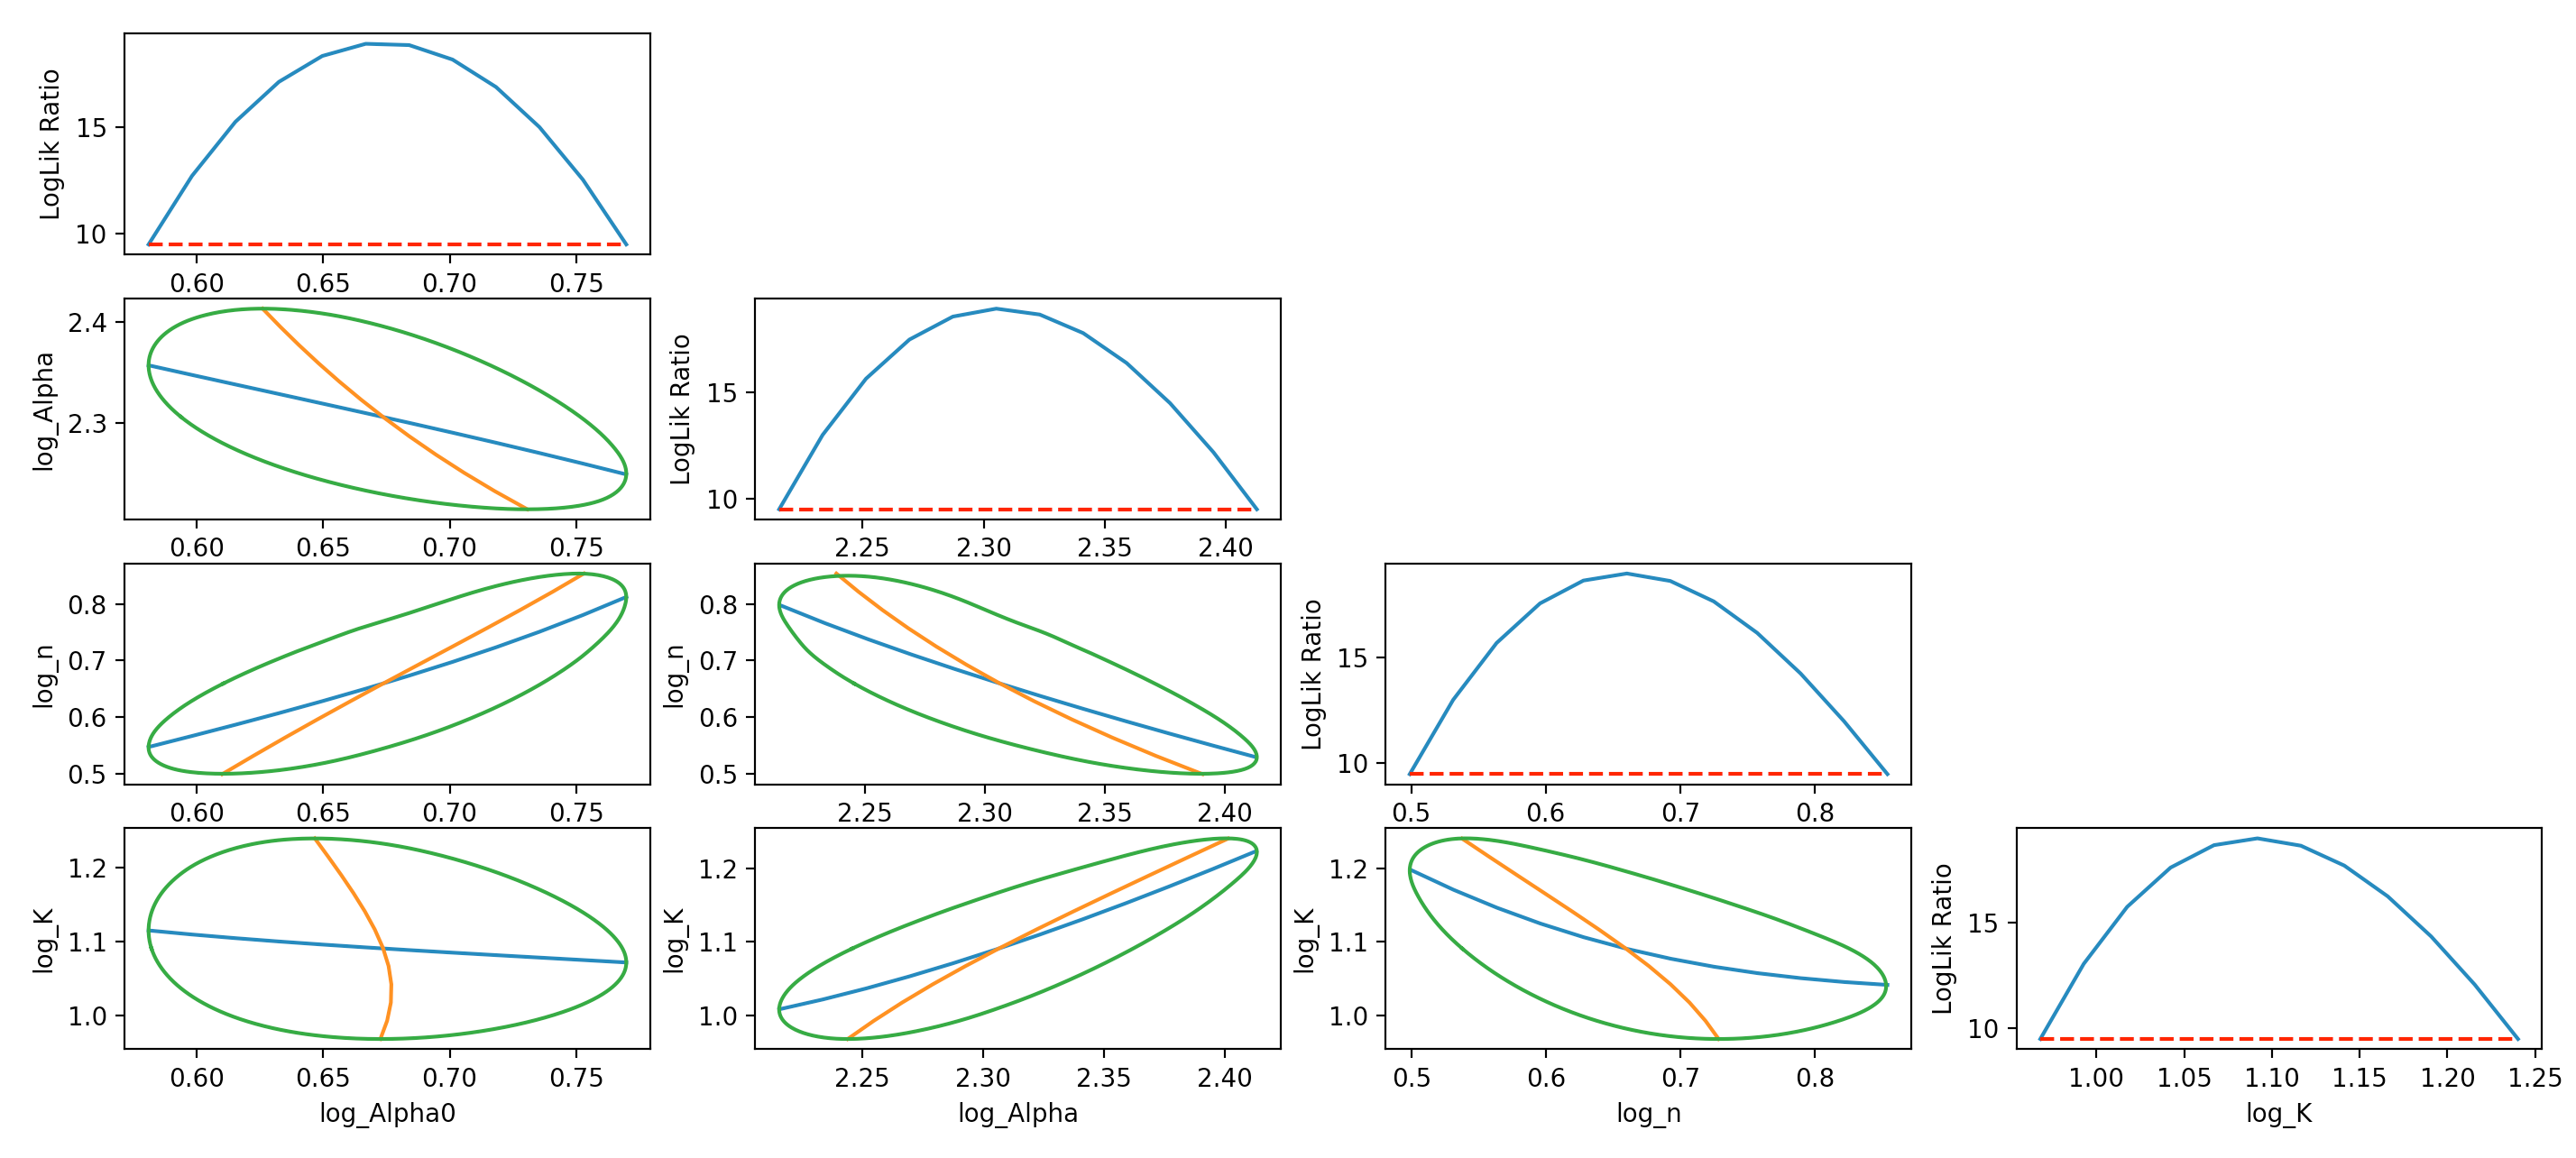
\includegraphics[scale=.3]{Images/ss_contours.png}
\caption{Diagnostic plots generated by the \texttt{fit()} function for the optogenetic dose-response model, including likelihood hood profiles, trace projections and contour projections.}
\label{fig:ss_contours}
\end{figure}
\noindent Likelihood based intervals are also generated during fitting and are given in the returned dataframe. The likelihood intervals for this example are shown in Figure \ref{fig:ss_lik_bnds}. 
\begin{figure}[htb!]
\centering
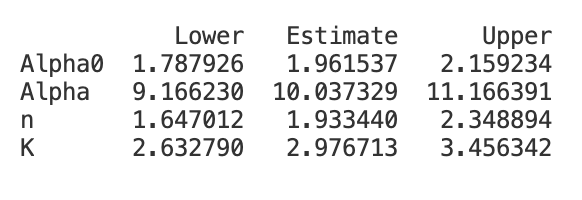
\includegraphics[scale=.7]{Images/ss_lik_bnds.png}
\caption{Output of the 95\% parameter confidence intervals generated using the profile likelihood functionality of the \texttt{fit()} function.}
\label{fig:ss_lik_bnds}
\end{figure}
\noindent Wald-type intervals can also be generated by using the \texttt{evaluate()} function as shown in Listing \ref{lst:ss_lst4}. The Wald intervals for this example are shown in Figure \ref{fig:ss_lik_bnds}. These intervals differ from those shown in Figure \ref{fig:ss_fim_bnds_update} only in that the parameter estimate has now shifted with the new data; this means the center of the interval moves but their widths are nearly the same under an exponential transformation (needed due to the log-transformed parameters).
\begin{figure}[htb!]
\centering
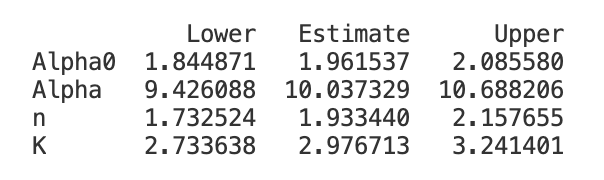
\includegraphics[scale=.7]{Images/ss_fim_bnds.png}
\caption{Updated 95\% Wald confidence intervals for the optogenetic dose-response model computed at the parameter estimates generated from the combined initial and optimal datasets. }
\label{fig:ss_fim_bnds}
\end{figure}
Comparing the likelihood-based and Wald-type intervals suggests reasonably good agreement in the intervals with the likelihood based intervals being slightly wider and more conservative. This lends support to the argument that the model has been calibrated with reasonable accuracy and that we are in a signal-to-noise regime where the approximations used in the design and diagnostics are accurate. In fact here, as we know the `true' data-generating parameters, we can confirm that the resulting estimate is very near the true value.

%Perhaps do a second dual input dual output dose response, with one discrete input like growth rate??
\subsection{Optimal Design for Dynamic Models}

% \textbf{Here I want to start with a simple ODE model, again with one input and maybe one state variable. I will carefully explain model settup in Casadi for dynamic models. I can then do a multi-state/timepoint multi input dynamic model.}
Encoding dynamic models in CasADi symbolics is somewhat more complicated than static models. The simplest method for doing so is to encode the numerical procedure itself as a symbolic structure. This has the advantage that the entire algorithm can be differentiated both for sensitivity and FIM computation, as well as within the optimizer. However this process can be confusing for first-time users and its scalability is limited to smaller dynamical systems. CasADi also offers external interfaces to third-party integration and sensitivity analysis packages such as CVODES as well as tools for creating differential-algebraic models \cite{Andersson2018}. In theory these can also be used in NLOED however they currently need further testing as of the date of writing. 

%\paragraph{RNA-Protein Two-state ODE Model} 
As a first example of a dynamic system we will address a two-state model of gene expression, including states for both mRNA and protein levels. The dynamic system can be written as
\begin{align}
\begin{aligned}
\frac{d\text{[RNA]}}{dt} =   \frac{\alpha}{1 +\frac{K}{\text{[Inducer]}}} - \delta \text{[RNA]}, \\
\frac{d\text{[Protein]}}{dt} =  \frac{\beta}{1 +\frac{L}{\text{[RNA]}}} - \gamma \text{[Protein]}.
\end{aligned}
\end{align}
Here expression of mRNA from the promoter is assumed to be controlled by an experimentally controlled inducer whose concentration is [Inducer] above. The state variable [RNA] is the mRNA concentration, the presence of which initiates translation of the corresponding protein. The concentration of the protien, [Protein], is the second state variable. Here $\alpha$, $\beta$, $K$, $L$, $\delta$ and $\gamma$ are parameters to be estimated. We assume the user is going to perform time series experiments on the proposed model and is looking to design such experiments for improved parameter estimation. 

\begin{listing}[H]
\begin{minted}[xleftmargin=\parindent,linenos,breaklines]{python}
#create state variable vector
states = cs.SX.sym('states',2)
#create control input symbol
inducer = cs.SX.sym('inducer')
#create parameter symbol vector
parameters = cs.SX.sym('parameters',6)
#log-transformed parameters
alpha = cs.exp(parameters[0]) 
K = cs.exp(parameters[1]) 
delta = cs.exp(parameters[2])
beta = cs.exp(parameters[3]) 
L = cs.exp(parameters[4]) 
gamma = cs.exp(parameters[5])
#create symbolic RHS
rhs = cs.vertcat(alpha*inducer/(K + inducer) - delta*states[0],
                 beta*states[0]/(L + states[0]) - gamma*states[1])
#create casadi RHS function
rhs_func = cs.Function('rhs_func',[states,inducer,parameters],[rhs])
\end{minted}
\caption{Code showing the creation of a CasADi function for the RHS of a two-state ODE model for the mRNA-protein dynamic model.}
\label{lst:dy_lst1}
\end{listing}
Encoding a dynamic model in CasADi symbolics for NLOED begins with the same import commands as the static models, see Listing \ref{lst:ss_lst0}. Following this the user begins by creating a symbolic expression and CasADi function for the right-hand side (RHS) of the dynamic system. Listing \ref{lst:dy_lst1} shows this process. In line 2, symbols are created for the state variables, mRNA and protein concentration. In line 4 a symbol is created for the inducer concentration. Line 6 shows the creation of a symbol vector for the model parameters. In lines 8-13, we perform a similar log transformation as that done in the static model, this ensures non-negativity of the named parameter values and improves numerical performance. In line 15-16, a symbol for the RHS of the system is created, containing symbolic expression for the equations given above. In line 18, a CasADi function is created mapping the current state and inducer levels as well as the parameters to the derivatives expressed by the RHS.

\begin{listing}[H]
\begin{minted}[xleftmargin=\parindent,linenos,breaklines,firstnumber=last]{python}
#time step size
dt = 1
# Create symbolics for RK4 integration, as shown in Casadi examples
k1 = rhs_func(states, inducer, parameters)
k2 = rhs_func(states + dt/2.0*k1, inducer, parameters)
k3 = rhs_func(states + dt/2.0*k2, inducer, parameters)
k4 = rhs_func(states + dt*k3, inducer, parameters)
state_step = states + dt/6.0 * (k1 + 2*k2 + 2*k3 + k4)
# Create a function to perform one step of the RK integration
step_func = cs.Function('step_func',[states, inducer, parameters],[state_step])
\end{minted}
\caption{Code showing the creation of a symbolic implementation of a fourth-order Runge-Kutta integrator using the RHS function for the mRNA-protein dynamic model.}
\label{lst:dy_lst2}
\end{listing}
Recall that CasADi functions can be used to return numeric values or new symbolic expressions depending on the inputs provided to them. The CasADi function for the RHS can therefore be used to create new symbols for numerical time-stepping of the state vector by a given integration method. In Listing \ref{lst:dy_lst2}, imitating examples given in the CasADi documentation, we implement a fourth-order Runge-Kutta algorithm (RK4) \cite{Andersson2018}. In line 20, the time step-size is set, and in lines 22-24, the four incremental slopes are computed using the RHS CasADi function. The inputs to the RHS function are symbols: \texttt{states}, \texttt{inducer}, \texttt{parameters}, and therefore the slopes: \texttt{k1}, \texttt{k2}, \texttt{k3}, and \texttt{k4} are also symbols. In line 26, the incremental slopes are combined to create a symbol for a full time step of the length set in line 20. In line 28, a CasADi function is created mapping the current state, inducer and parameter values to the next state values.

\begin{listing}[H]
\begin{minted}[xleftmargin=\parindent,linenos,breaklines,firstnumber=last]{python}
# create a symbol for the initial inducer level
initial_inducer = cs.SX.sym('init_inducer')
#define the steady state initial states in terms of the initial inducer
init_mrna = (alpha/delta)*initial_inducer/(K+initial_inducer)
ini_prot = (beta/gamma)*init_mrna/(L+init_mrna)
# zip the initial states into a vector
initial_states = cs.vertcat(init_mrna, ini_prot)
#create a vector for inducer levels in each control interval
inducer_vector = cs.SX.sym('inducer_vec',3)
#merge all inducer levels into a single experimental inputs vector
inputs = cs.vertcat(initial_inducer,inducer_vector)
\end{minted}
\caption{Code showing how the initial conditions for the mRNA-protein model's steady states are encoded symbolically. Composition of the experimental input vector is also illustrated.}
\label{lst:dy_lst3}
\end{listing}
The RK4 time-stepping CasADi function, \texttt{step\_func()}, allows us to build up integrated solution curves of the model system as symbolic expressions. At this point we have a fair degree of flexibility in how the problem will be posed to NLOED via the \texttt{Model} class. We specifically need to choose how the initial conditions and inducer concentration throughout a single time series are encoded as NLOED model inputs, and how the state variables at various time points throughout the series are encoded as model observation variables. An example of our chosen formulation of the problem is shown in Listing \ref{lst:dy_lst3} and \ref{lst:dy_lst4}. We have opted to have the system start at steady state with respect to a variable input level; in Listing \ref{lst:dy_lst3}, lines 30-35, the initial conditions are implemented symbolically. In line 30, a symbol, \texttt{initial\_inducer}, is created for the initial inducer level. In lines 32-33 we compute the steady state values of the two state variables in terms of the initial inducer concentration. In line 35, we concatenate the initial state variables into a single vector, \texttt{initial\_states}, containing the initial states of the system. In line 37, we create a vector, \texttt{inducer\_vector}, containing the three inducer levels, one for each of the three control intervals over the duration of the experiment (see further discussion below). In line 39 we concatenate the \texttt{initial\_inducer} and \texttt{inducer\_vector} to form the overall set of inputs for the designed time-series experiment. This means each experiment has four experimental inputs, the initial inducer concentration to which the system starts in steady state, and three other inducer concentrations applied sequentially through the experimental duration.

\begin{listing}[H]
\begin{minted}[xleftmargin=\parindent,linenos,breaklines,firstnumber=last]{python}
#3 samples per cntrl interval, 3 cntrl intervals
#control intervals are 1+2+3=6 steps long:
#  cntrl_int1    cntrl_int2    cntrl_int3
#|-1---2-----3||-1---2-----3||-1---2-----3|
#set number of control intervals
num_cntrl_intervals = 3
#define a sample pattern to apply in each control interval
sample_pattern= [1,2,3] 
#lists to store symbols for each sample point, and times of each sample
sample_list, times = [], []
# set the initial states and initialize the step counter
current_state, step_counter = initial_states, 0
#loop over control invervals
for interval in range(num_cntrl_intervals):
  # loop over sample pattern
  for num_stps in sample_pattern:
    #iterate steps indicated by sample pattern
    for k in range(num_stps):
      #propagate the state variables via integration
      current_state = step_func(current_state, inducer_vector[interval], parameters)
      step_counter+=1
    #save the state symbols and times of each sample
    sample_list.append(current_state)
    times.append(step_counter*dt)
\end{minted}
\caption{Code showing how the symbolic integration is used to implement a specific sampling and observation pattern, and how observation variables for various states and time points are collected.}
\label{lst:dy_lst4}
\end{listing}
Having prescribed the model inputs we now need to collect the observation variables (at multiple time points) into an observation list for the \texttt{Model} constructor. To do so we must increment over the time series using the RK4 time stepping, implementing the inducer control scheme and collecting time points through the looping process. This procedure is shown in Listing \ref{lst:dy_lst4}. The current time-stepping algorithm is ideal for a step-wise input in the inducer concentration and we choose to implement three control intervals, meaning that each time course can have three different levels of inducer concentration, occurring sequentially each for the same length of time. In line 45, we therefore set the number of control intervals to three. In our case, the control intervals are assumed to be relatively long compared to the relaxation time of the system, as such we will want the option to select several observation time points within each sampling interval. Here we choose to place candidate observation points at one, two and three time steps after the beginning of the control interval. In line 47 we create a list containing the number of time steps to advance before taking an observation. Both the number of control intervals, and the time steps before observation, can be used to construct the looping structure to iterate over the experiment. In line 49, we create lists to store CasADi symbols for the observed state at various time points as well as the times at which these occur. In line 51, we initialize the system state to the steady state values in the \texttt{initial\_state} variable and set the step counter to 0. Beginning on line 53, we loop over the three control intervals; each pass through this loop integrates a single control interval over which there is a constant inducer level. On line 57 we loop over the \texttt{sample\_pattern} array, such that the loop variable \texttt{num\_stps} will contain the number of integration steps that need to be incremented. This loop effectively iterates over observations within each control interval. As there are three possible observation within each control interval, this loop will repeat three times for each control interval; however, note that the time between observations is not the same, as set by the \texttt{sample\_pattern} array. In line 57, we enter the time stepping and iterate over the specified number of steps using \texttt{step\_func}. In the time stepping loop, we apply the RK4 step function in line 59 to the current state vector in \texttt{current\_state} with the prescribed inducer level specified by \texttt{inducer\_vector[interval]}. The step counter is also incremented in line 60, to track the number of RK4 steps taken and thus the time elapsed. In line 62 we store the state vector, which at this point corresponds to an observation time point; the time is also computed and recorded in line 63.

\begin{listing}[H]
\begin{minted}[xleftmargin=\parindent,linenos,breaklines,firstnumber=last]{python}
# create list for observation structure 
observation_list= []
#create list to store response names
observation_names, observation_type, observation_times = [], [], []
# loop over samples (time points)
for i in range(len(sample_list)):
  #create a unique name for mrna and prot samples
  mrna_name = 'mrna_'+'t'+"{0:0=2d}".format(times[i])
  prot_name = 'prot_'+'t'+"{0:0=2d}".format(times[i])
  #create mean and var tuple for mrna and prot observ.
  mrna_stats = cs.vertcat(sample_list[i][0], 0.005)
  prot_stats = cs.vertcat(sample_list[i][1], 0.005)
  #create casadi function for mrna and prot stats
  mrna_func = cs.Function(mrna_name,[inputs,parameters],[mrna_stats])
  prot_func = cs.Function(prot_name,[inputs,parameters],[prot_stats])
  #append the casadi function and distribution type to obs struct
  observation_list.extend([(mrna_func,'Normal'), (prot_func,'Normal')])
  #store observation names, useful for plotting
  observation_names.extend([mrna_name,prot_name])
  #store observation type
  observation_type.extend(['RNA','Prot'])
  #store observation time
  observation_times.extend([times[i]]*2)
\end{minted}
\caption{Code showing the assembly of the \texttt{observ\_list} argument for use in the \texttt{Model} class constructor call for the mRNA-protein dynamic model. }
\label{lst:dy_lst5}
\end{listing}
After completing the loop structure shown in Listing \ref{lst:dy_lst4}, the result is a list, \texttt{sample\_list}, containing symbols for the each state variable at the observation time points under consideration. It remains for us to construct CasADi functions for each of these symbols, before they can be passed to the \texttt{Model} constructor via an observation list. We also need to specify the distribution type assumed for each state variable; here we assume a normal distribution with constant variance to keep the model simple for illustrative purposes. Listing \ref{lst:dy_lst5} provides a loop in which the symbols list is used to construct CasADi functions each of which is then stored in an observation list for passage to the \texttt{Model} constructor. In line 65, the \texttt{observation\_list} list is declared and in lines 67 several other lists are initialized for storing the observation name, type (RNA or protein) and time; these are valuable for plotting and organizing data later. On line 69, the loop for building up the observation list begins; this loop iterates over each element in the sample list containing the observation symbols. In lines 71-72, each state's observation is given a unique string name, marking its type and time. On lines 74-75, the state observation statistics (mean and variance) are concatenated together. On lines 77-78 we construct CasADi functions mapping experimental inputs (the various inducer levels) and the model parameters to the observation statistics. On line 80, we append the CasADi functions in tuples with the \texttt{Normal} label, to the observation list. In lines 83-86 we also store the auxiliary information for plotting and data export in the previously declared lists. 
\begin{listing}[H]
\begin{minted}[xleftmargin=\parindent,linenos,breaklines,firstnumber=last]{python}
#list the inpit and parameter names
input_names = ['Init_Inducer','Inducer_1','Inducer_2','Inducer_3']
parameter_names = ['log_Alpha','log_K','log_Delta','log_Beta','log_L','log_Gamma']
#instantiate the model object
model_object = Model(observation_list, input_names, parameter_names)
\end{minted}
\caption{Code showing the creation of an NLOED \texttt{Model} object for the mRNA-protein dynamic model.}
\label{lst:dy_lst6}
\end{listing}
Following the creation of the observation structure in the previous loop, we are ready to create the NLOED model. Shown in Listing \ref{lst:dy_lst6}, in lines 88 and 89 we declare the input and parameter names and on line 91 we create an NLOED model object named \texttt{model\_object} using the NLOED \texttt{Model} class constructor. 

\begin{figure}[htb!]
\centering
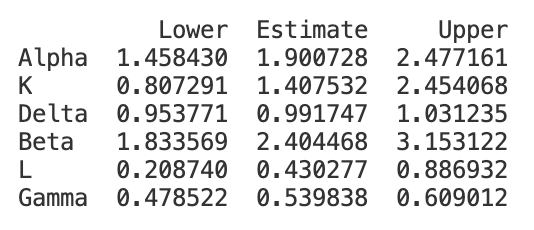
\includegraphics[scale=.7]{Images/dy_init_bnds.png}
\caption{Output of the 95\% Wald confidence intervals under the initial dataset for the mRNA-protein dynamic model, computed using the \texttt{evaluate()} function.}
\label{fig:dy_init_bnds}
\end{figure}
We can use code similar to code listings \ref{lst:ss_lst3}, \ref{lst:ss_lst4} and \ref{lst:ss_lst5} in the static model to for fitting, generating Wald-type confidence intervals and prediction bounds. In this example, we assume an initial dataset with a single observation at each possible time point during a single time course. We assume the time course begins with an initial inducer concentration of 0 and the subsequent three inducer levels are set to 1, 0 and 3 respectively. Fitting is done as in the static model using the \texttt{model\_object} and the \texttt{fit()} function. Wald intervals are shown in Figure \ref{fig:dy_init_bnds}. The size of these bounds relative to the magnitude of the parameters is reasonably large and could be improved. 
\begin{figure}[htb!]
\centering
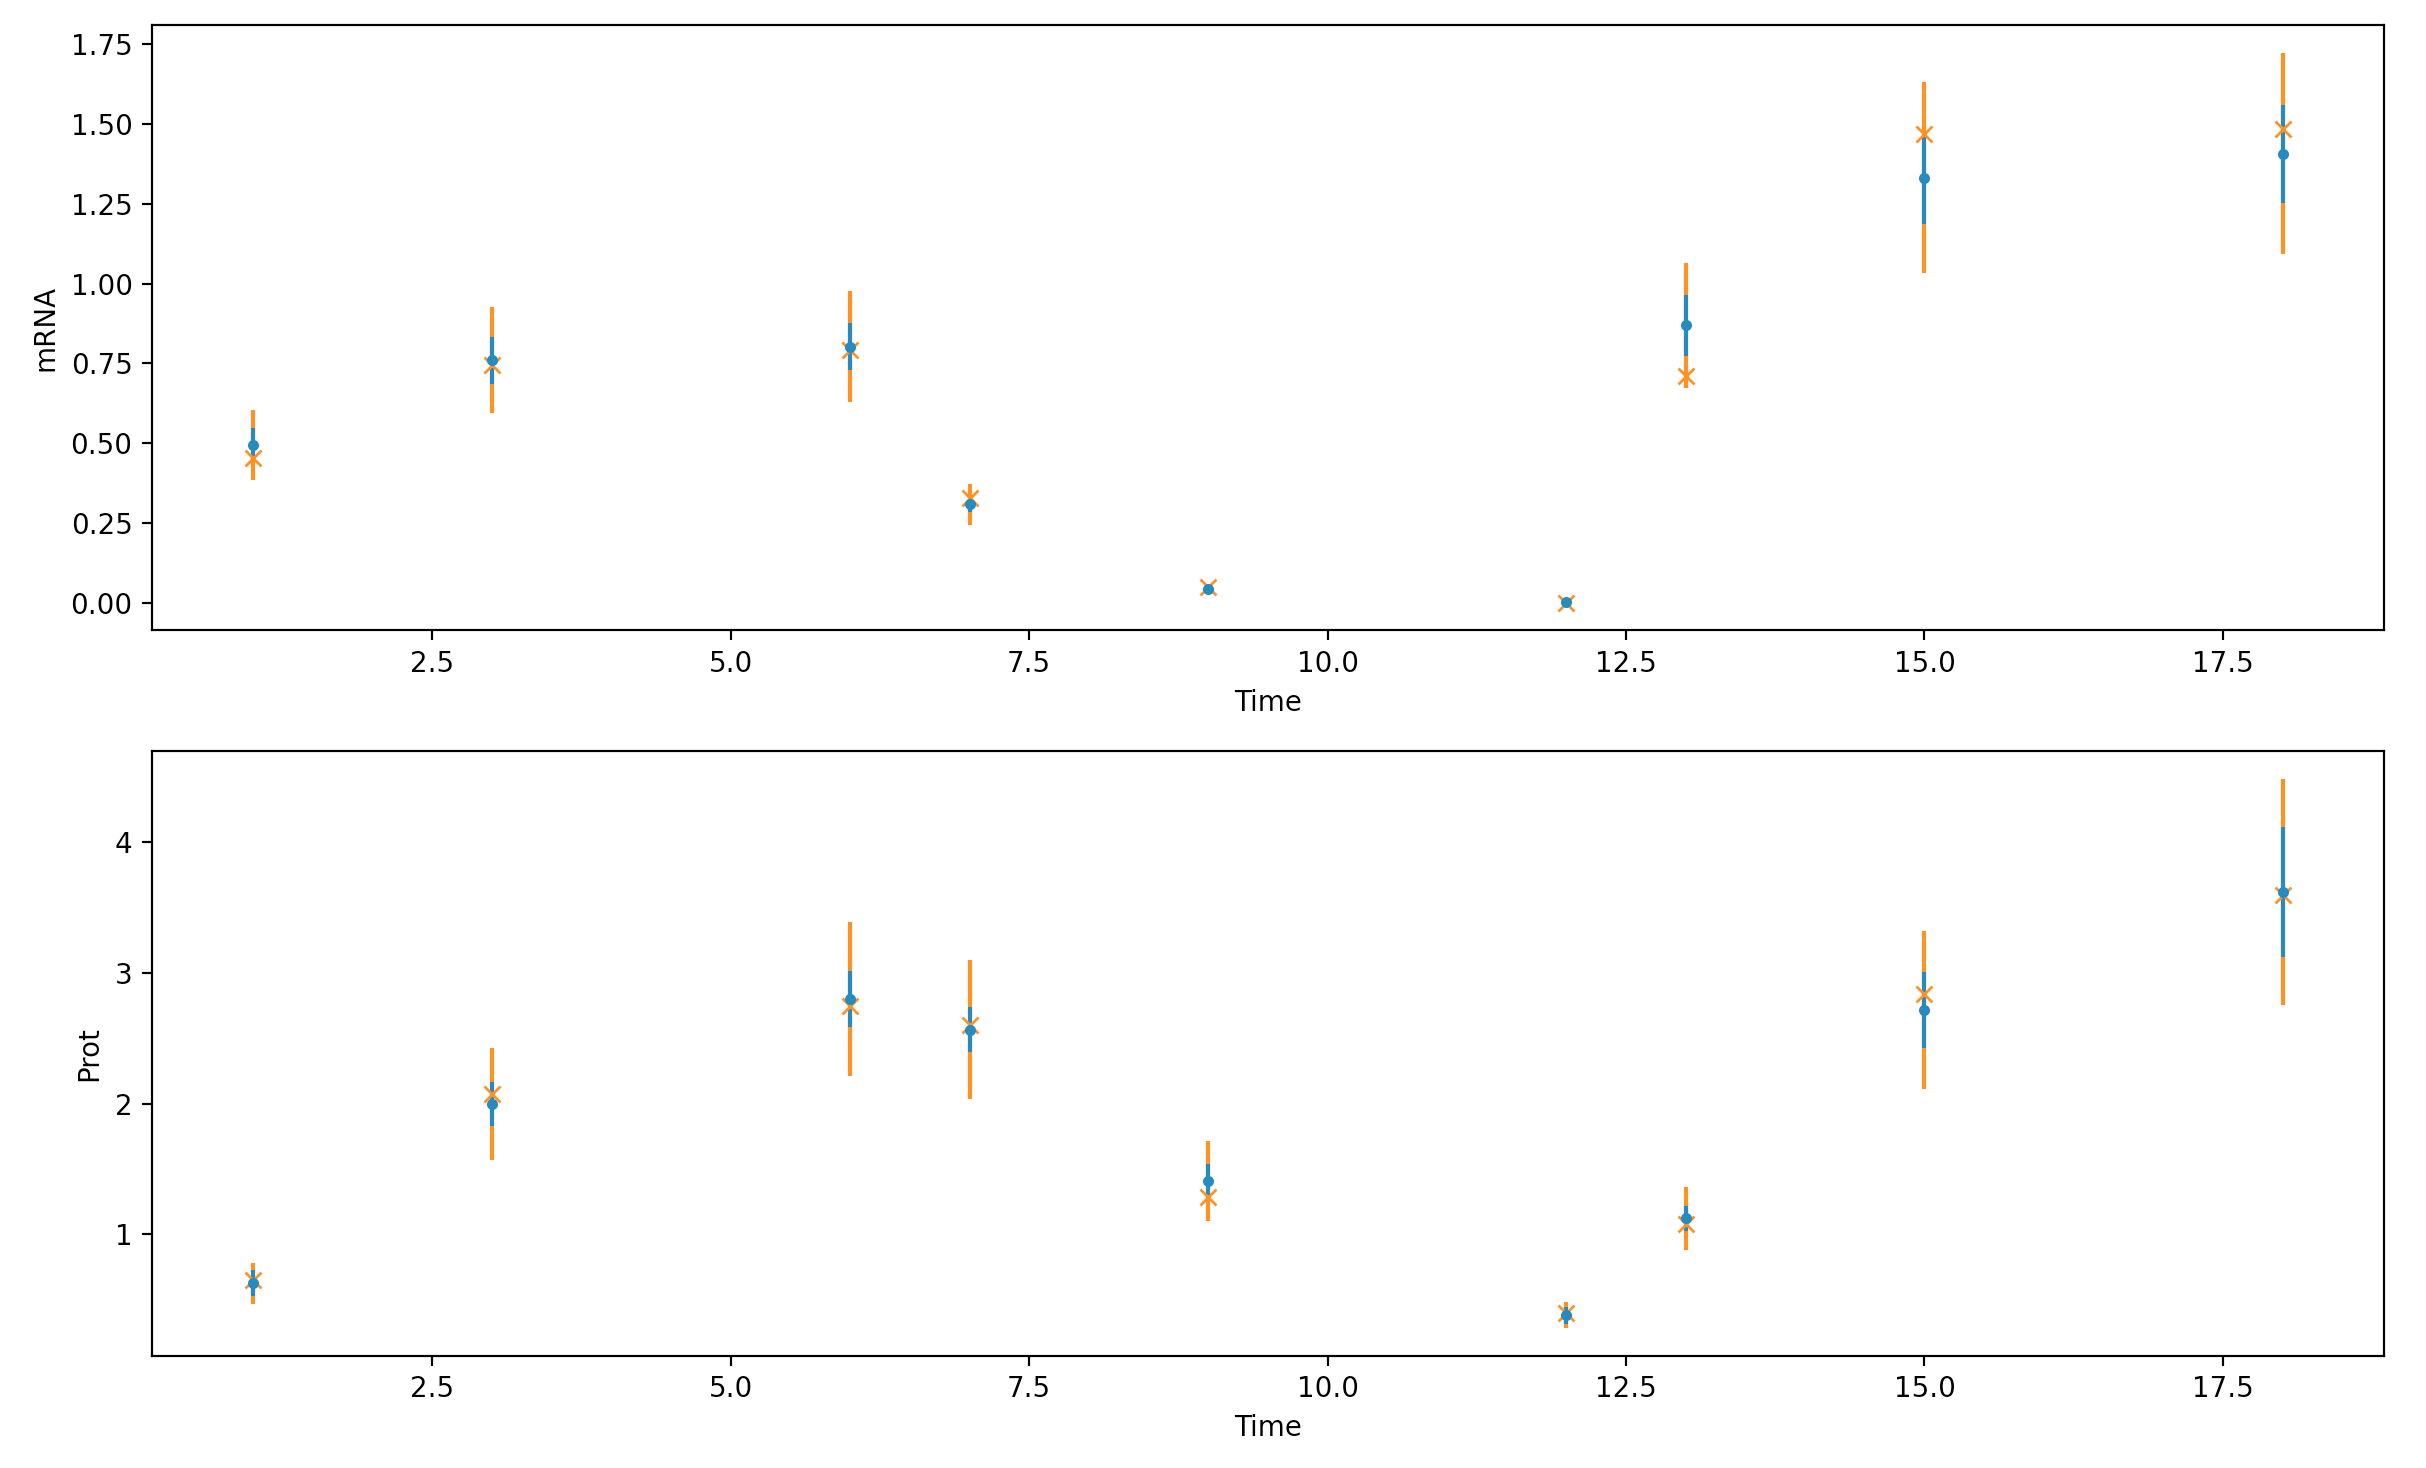
\includegraphics[scale=.3]{Images/dy_init_pred.png}
\caption{Prediction of the mean mRNA and protein levels, along with the 95\% prediction and observation intervals generated with the \texttt{predict()} function for the mRNA-protein dynamic model.}
\label{fig:dy_init_pred}
\end{figure}
Prediction and observation intervals can also be generated using calls to the \texttt{evaluate()} function to generate parameter covariances, and calls to the predict function to generate the mean and interval information. Figure \ref{fig:dy_init_pred} depicts the predicted mean response at each observation point in the initial experiment (shown as blue dots). Data from a simulation of the initial experiment is also shown (orange x's), along with prediction intervals for the mean under parameter uncertainty (blue bands) and observation intervals for the data under both sampling and parameter uncertainty (orange bands).

\begin{listing}[H]
\begin{minted}[xleftmargin=\parindent,linenos,breaklines,firstnumber=last]{python}
#set all inducer inputs as continuous
continuous_inputs={'Inputs':['Init_Inducer','Inducer_1','Inducer_2','Inducer_3'],
                   'Bounds':[(.01,5),(.01,5),(.01,5),(.01,5)],
                   'Structure':[['I0','I1','I2','I3']]}
#create the fixed design dictionary
fixed_dict ={'Weight':0.5, 'Design':init_design}
# generate the optimal design object
design_object = Design(model_object,fit_params,'D',
                       fixed_design = fixed_dict,
                       continuous_inputs = continuous_inputs)
#set the sample size to 18
sample_size = 18
#generate a rounded exact design 
exact_design = design_object.round(sample_size)
\end{minted}
\caption{Code showing the instantiation of a \texttt{Design} object for the mRNA-protein model, as well as the generation of an exact design with a sample size of 18.}
\label{lst:dy_lst7}
\end{listing}
To generate an optimal experiment we need to instantiate a \texttt{Design} instance; Listing \ref{lst:dy_lst7} shows this process. In lines 93-95 we specify that all inputs will be treated as continuous, bounded between 0.1 and 5 and that a single inducer profile will be optimized. In line 97, we create a \texttt{fixed\_design} dictionary and include the initial design (contained in the dataframe \texttt{init\_desgin}) and weight it at 0.5. This weighting of the initial design implies the optimal design will be implemented with the same number of observations, 18, as the initial data. In lines 99-101, we call the \texttt{Design} constructor and instantiate the \texttt{design\_object}. in line 103, we set the sample size to 18, and in line 105 we generate an exact design with the \texttt{round()} function.

\begin{figure}[htb!]
\centering
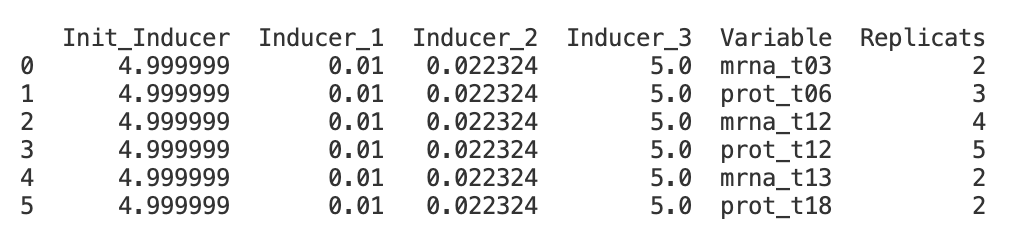
\includegraphics[scale=.7]{Images/dy_exact.png}
\caption{Output of the optimal exact design generated for the mRNA-protein dynamic model.}
\label{fig:dy_exact}
\end{figure}
\noindent The optimal design generated from this process is shown in Figure \ref{fig:dy_exact}. The resulting design sets an initial inducer concentration of 5 and then drops it to the minimum of 0.01 in the first control interval. In the second control interval, the inducer is increased slightly to 0.022 and in the final interval it is again increased to the maximum of 5.
\begin{figure}[htb!]
\centering
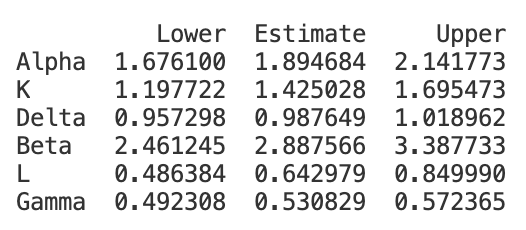
\includegraphics[scale=.7]{Images/dy_opt_bnds.png}
\caption{Updated 95\% confidence intervals for the mRNA-protein model, generated using the \texttt{evaluate()} function and the combined initial and optimal designs.}
\label{fig:dy_opt_bnds}
\end{figure}
Various protein and RNA measurements are taken at different times (coded in the \texttt{Variable} column) and replicate numbers. This type of design is possible if multiple biological replicates can be run with a shared inducer level. For example light or temperature induced systems may be suitable for this type of input and replication structure.
\begin{figure}[htb!]
\centering
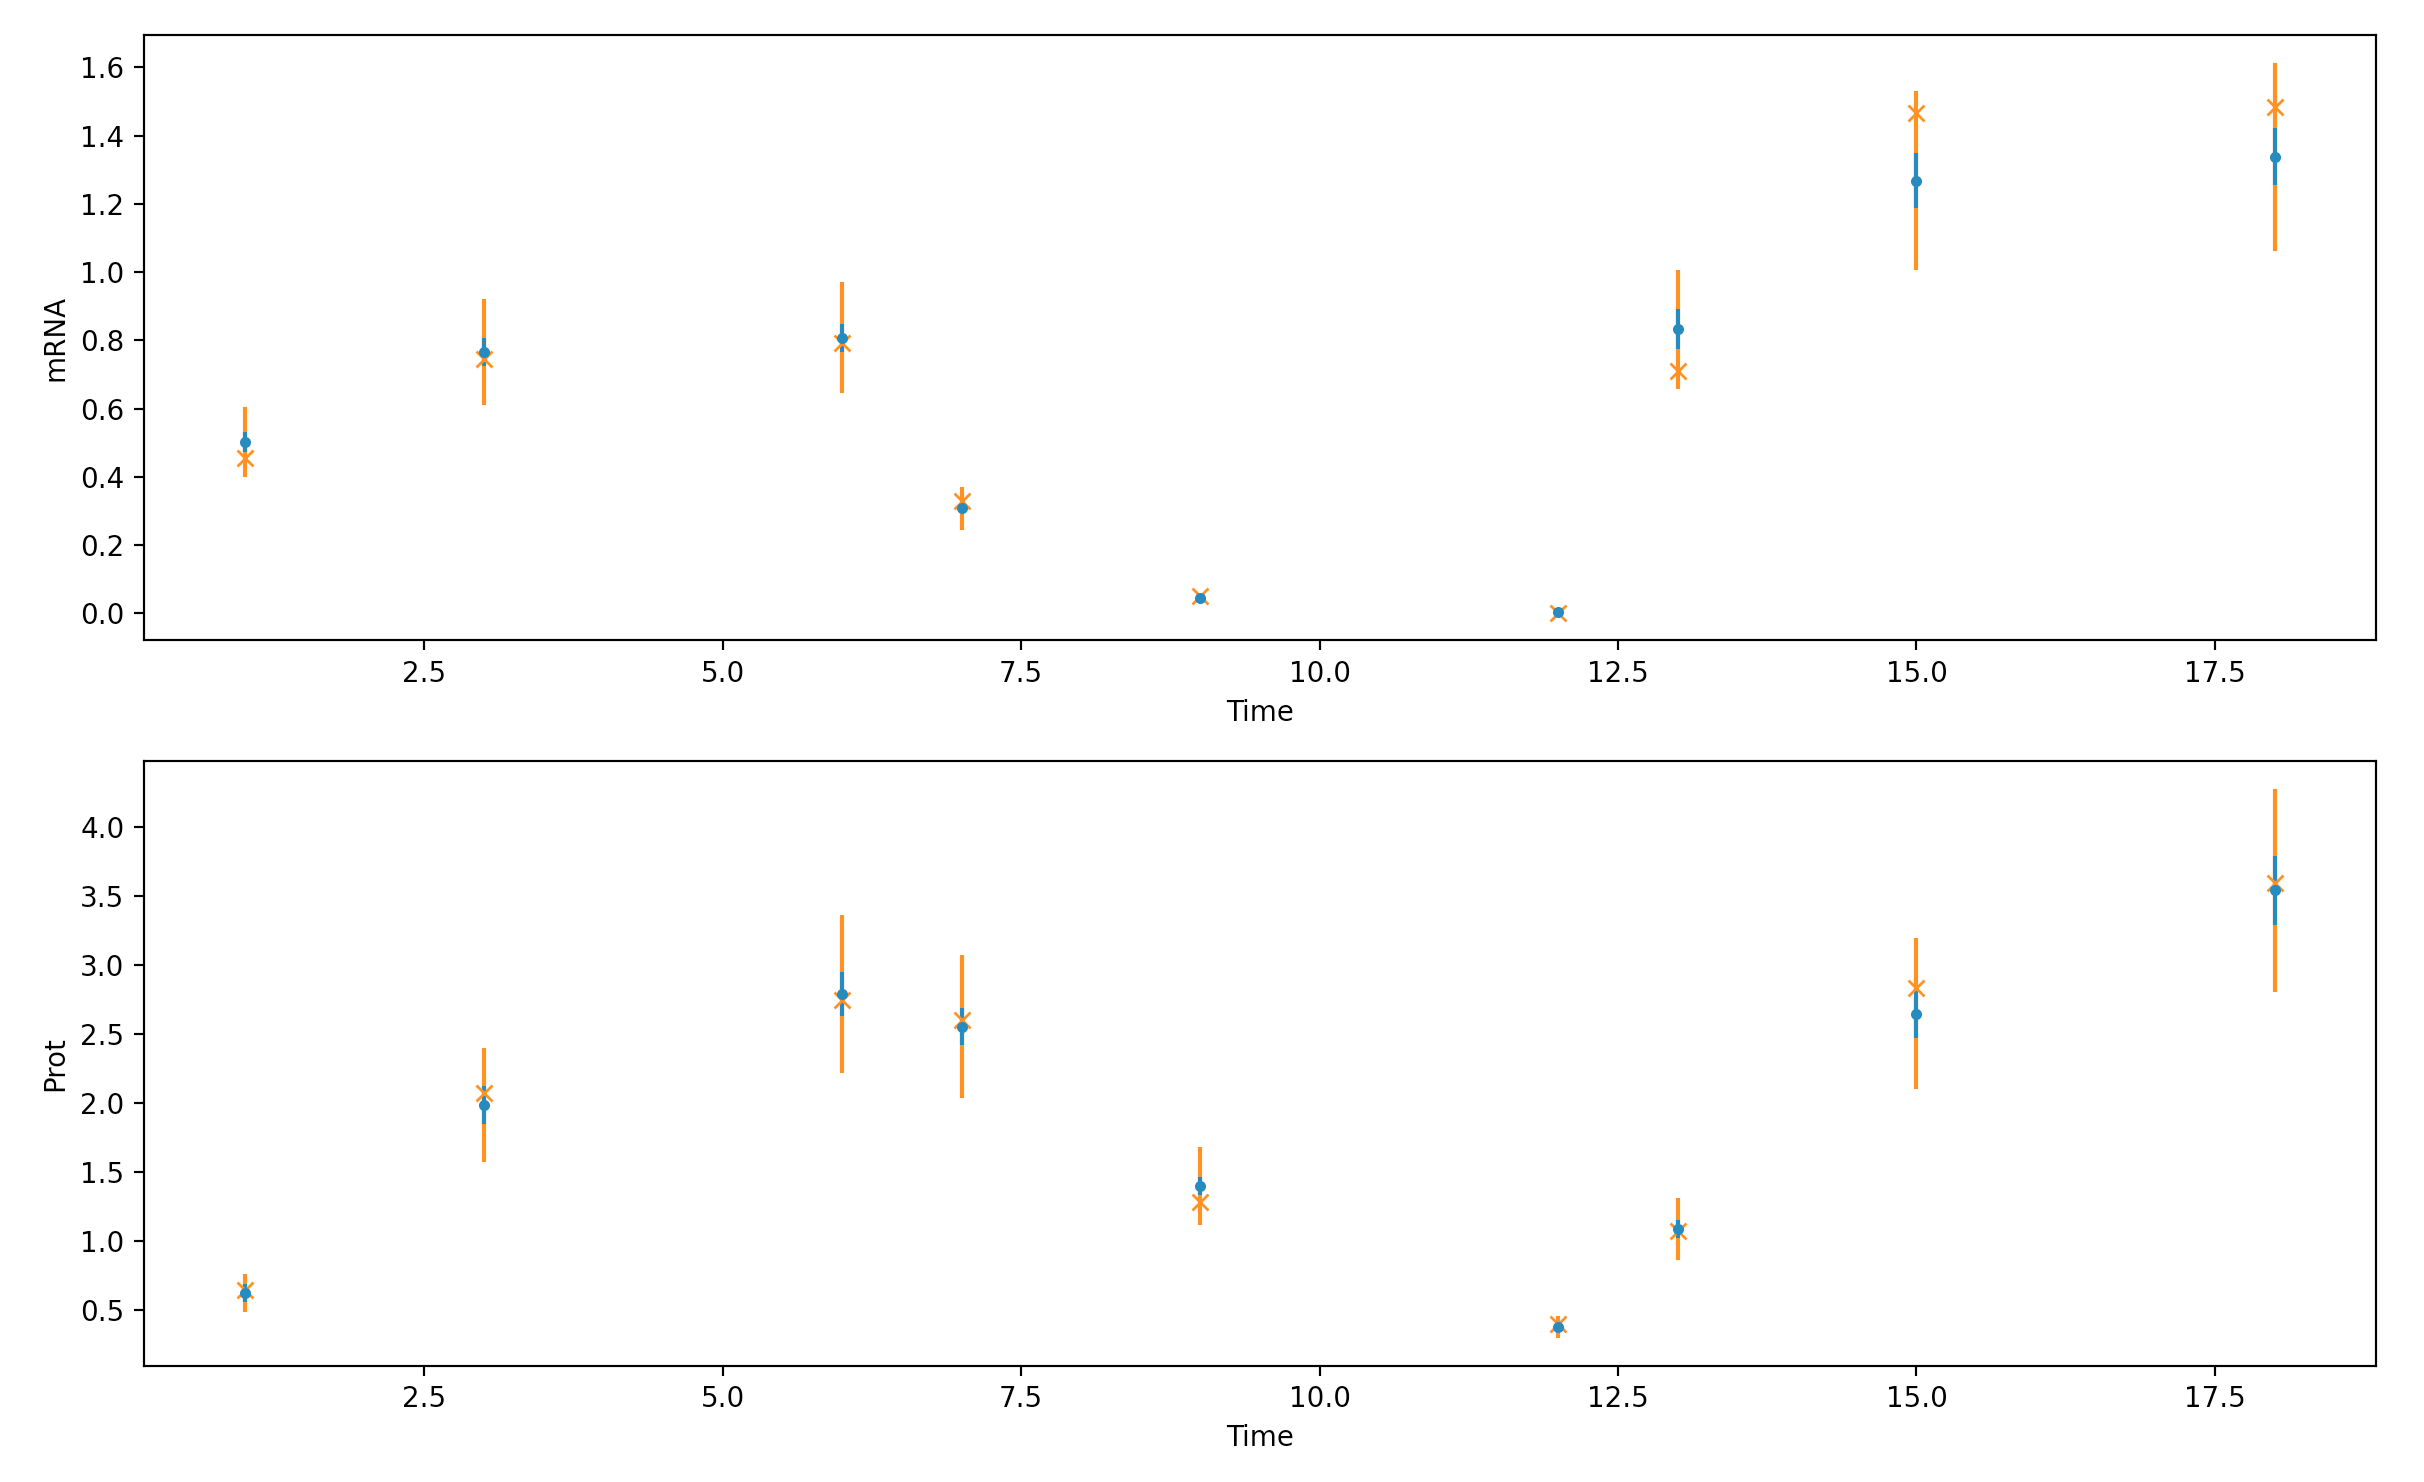
\includegraphics[scale=.3]{Images/dy_opt_pred.png}
\caption{Updated 95\% prediction and observation intervals for the mRNA-protein model, generated using the \texttt{predict()} function under the covariance found using \texttt{evaluate()} applied to the combined intitial and optimal designs.}
\label{fig:dy_opt_pred}
\end{figure}
In these situations multiple cultures can be grown (and thus multiple replicates sampled) in the same inducer sequence within their incubator or light box. If the user instead wishes to optimize an experiment where each replicate can have its own unique inducer course but multiple replicate observations cannot be made at each time point, the user can use the \texttt{LockWeights} option of the \texttt{Design} class and a different continuous input structure. However use of the \texttt{LockWeights} option prohibits time point selection and the user must use a fixed sampling schedule. After implementing the optimal design we can update the Wald intervals, shown in Figure \ref{fig:dy_opt_bnds}. Here we see that interval sizes have shrunk. Figure \ref{fig:dy_opt_pred} shows the new prediction and intervals for the original dataset. Here we see that the prediction intervals (blue bands) have shrunk somewhat from the initial data collection. Further improvements would be expected if the sample size was increased for the optimal design. 


% Example, three time points all sampled always, choose mixture of runs to do with continuous input controls (init/final induction), external settings (i.e. growth rate/temp)

% Example, mrna and protein choose sample timepoints for a single run with variable controls

% \subsection{Other Workflow Elements}
% \textbf{This section is somewhat optional but I wanted to add some examples of other package uses. Examples include; 1)simulation studies (which uses the sample() and fit() functions), 2) evaluating a design and using the resulting covariance matrix to generate prediction uncertainties (this uses the evaluate() and predict() functions together), and power analysis (which shows how to choose a sample size for a specific goal). I would do these for a very simple model and they would be there to illustrate ideas for how to creatively use the package for various goals. }
% \paragraph{Sampling and Fitting}
% Multiplexing for batch data generating (used internally for MC and can be used externally for setting up simulation studies like those used in previous chapters.
%  Uncertainty assesment via profile lik
%  sample plots pic
%  \begin{minted}[xleftmargin=\parindent,linenos,breaklines,firstnumber=last]{python}
% # GENERATE SAMPLE DATA & FIT MODEL
% #generate some data, to stand in for an initial experiment
% data = nloed_model.sample(exact_design,np.log(true_param))
% print(data)
% #pass some additional options to fitting alglorithm, including Profile likelihood
% fit_options={'Confidence':'Intervals',  #NOTE: ISSUE WITH PROFILES HERE
%              'InitParamBounds':[(-1,4),(-1,4),(-1,4),(-1,4)],
%              'InitSearchNumber':7,
%              'SearchBound':5.}
% #fit the model to the init data
% fit_info = nloed_model.fit(data, options=fit_options)
% print(fit_info)
% fit_params = fit_info['Estimate'].to_numpy().flatten()
% \end{minted}
% \paragraph{Design Evaluation and Prediction}
% FIM, Cov, Bias and MSE via asymptotics or Monte Carlo
% \begin{minted}[xleftmargin=\parindent,linenos,breaklines,firstnumber=last]{python}
% ##################################
% # EVALUATE DESIGN & PREDICT OUTPUT
% ##################################
% #get estimated covariance, bias and MSE of parameter fit (use asymptotic method here) 
% opts={'Covariance':True,'Bias':True,'MSE':True,'SampleNumber':100}
% diagnostic_info = nloed_model.evaluate(exact_design,fit_params,opts)
% print(diagnostic_info)
% #generate predictions with error bars fdor a random selection of inputs)
% prediction_inputs = pd.DataFrame({ 'Light':np.random.uniform(0,5,10),
%                                 'Variable':['y']*10})
% cov_mat = diagnostic_info['Covariance'].to_numpy()
% pred_options = {'PredictionInterval':True,
%                 'ObservationInterval':True,
%                 'Sensitivity':True}
% predictions = nloed_model.predict(prediction_inputs,
%                                   fit_params,
%                                   covariance_matrix = cov_mat,
%                                   options=pred_options)
% print(predictions)
% \end{minted}
% \paragraph{Design Comparison and Power Analysis}
%  Possible 

\section{Discussion}

%BPI: MAYBE REMOVE PLANNED FEATURE FROM TEXT, BUT DEFINITELY HIGHLIGHT WHAT NEEDS TO BE DONE HERE SO IT IS CLEAR WHAT IS MISSING

%In future releases this argument will accept other FIM based objectives such as D$_s$-optimal and A-optimal objectives. Each of these prospective features are near completion and expected to be included in the initial release.

%In future versions, the number of rounding methods will be extended, along with options to return the set of designs generated by a rounding method that terminates with a non-unique design. Tools to rank and quantify the various designs according to their loss in optimality compared to the relaxed design will also be included. 

%In future releases, this local analysis will also be supplemented by allowing \texttt{parameters} to also accept either mean and covaraiance information for a normal prior, or a list of equally-likely candidate parameter values. Averaged optimal designs can then be generated with respect to the given parameter uncertainty by using the sigma-point method \cite{schenkendorf2009optimal} or related approaches  -- these features are also still in development. 

%In the current implementation, the \texttt{models} argument can also  

The current version of NLOED implements much of the core functionality and many important supplemental features, however I intend to add a number of additional features before the initial release. Currently more testing and further user-interface design is needed before the NLOED package can support optimal design over model or parameter uncertainty. Specifically, in future releases the \texttt{models} argument to the \texttt{Design} class will accept a list of \texttt{Model} instances as along as they have the same input structure. With a list of \texttt{Model} instances passed, the resulting design is optimized for an average objective across all of the models. This model averaging provides designs that can be used to fit any of the candidate models, providing robustness to model uncertainty (but not necessarily addressing model selection). In future releases, the local design optimization at a nominal parameter vector, $\bar{\bm{\theta}}$, will also be supplemented with a pseudo-Bayesian approach which will allow for design optimization over a weighted average of several candidate parameter points \cite{schenkendorf2009optimal}. To accomplish this the \texttt{parameters} argument to the \texttt{Design} class will accept either mean and covaraiance information for a normal prior, or a list of weighted candidate parameter vectors. %Averaged optimal designs can then be generated with respect to the given parameter uncertainty by using the sigma-point method  or related approaches  -- these features are also still in development. 
Much of the numerical structures for these model and parameter uncertainty features have already been implemented but they need further testing and documentation. Also, while the D-optimal objective is widely used and useful, support for D$_s$-optimal designs is also planned for the initial release as the D$_s$ objective facilitates designs targeting specific parameters sets or even model selection in nested models \cite{atkinson1992optimum}. The \texttt{power()} function of the \texttt{Design} class remains to be implemented; while not required for optimal design it provides important tools for assessing the sensitivity of confidence intervals to the overall sample size. I also plan to provide greater flexibility and more user feedback within the \texttt{round()} function in the \texttt{Design} class so the user has more guidance and control over the generation of exact designs. Lastly, I hope to improve the numerical stability of model fitting, likelihood profiling and the design optimization algorithms through additional testing and tuning of the default algorithm settings. 
%-improving rounding (more options, some within rounding optimization, comparison methods for non-unique roundings etc.)

%One iterpretation, Package viewed as Bayesian laplace approximation with FIM as normal covariance, thus prediction intervals are like posterior predictive Ie for checks, iterative is bayesian updating 
%-post-hoc optimization

I also have several secondary objectives for package extensions. These include adding diagnostics based explicitly on the general equivalence theorem, which in special cases can be used as a powerful tool for checking optimality and understanding design structure \cite{kiefer1960equivalence,atkinson1992optimum}.
I also aim to improve the user experience in implementing dynamic models, including helper functions for implementing the CasADi symbolic integration and for extracting data and design information at various time points. While NLOED already supports a large variety of experimental constraints, in future version I plan to allow the user to place non-linear constraints on continuous inputs as well as the sampling weights. I also hope to integrate other powerful numerical tools available through CasADi's interfaces, including other optimization, numerical integration and sensitivity analysis packages (i.e. CVODES), and tools for constrained and differential-algebraic systems. Using these tools I would like to expand support and code optimization for models involving implicit functions, optimization and differential-algebraic systems in the future.

%-adding coordinate exchange and grid refinment
%-include designs for random effects


Optimal experimental design has a long history of research; algorithms for optimizing designs for non-linear, dynamic models dates back to the 1950's, see work by Box and Lucas \cite{box1959design}. In over a half-century of study, the area has been well researched and the theory, as well as numerical procedures, for optimal design thoroughly explored. In many ways it is a mature field, with few prospects for revolutionary new ideas. However, it remains a challenge to translate the existing body of knowledge into practice for an evolving experimental discipline like systems biology; updated tools that focus on usability and easy-adoption are needed. While systems biology makes use of (psuedo-)mechanistic models and designed experimentation, model parameters are often only accessible via fitting. This situation poses unique challenges as the models can have complicated non-linear structures with a variety of observables, like in more fundamental sciences, but model calibration and testing often require statistical tools more common in econometrics and other medical or social sciences. Systems biology also includes a wide range of practitioners, from experimentalists with non-quantitative backgrounds from many areas of biology, to more quantitative experts from fields like physics, engineering, computer science, and mathematics. Translating OED ideas into a set of tools that is easy to use yet flexible for such a wide range of models and users is difficult, especially as even the quantitative practitioners may lack familiarity with the advanced statistical diagnostics and fitting concepts on which OED relies. 

The NLOED package attempts to address some of the opportunities and challenges listed above. While other packages exist, NLOED supports a unique blend of models and numerical algorithms specifically suited to systems biology models; with special consideration for the diversity of model structures (non-linear, dynamic, multi-input/output) and numerical implementations (numerically integrated and even implicitly defined models). NLOED also incorporates these tools with an updated toolset, making use of automatic differentiation and state-of-the-art open-source optimization via CasADi. This provides a flexible and extensible platform on which to build future capabilities. The package has been written in open-source object-oriented Python with special attentions being paid to interoperability with other third-party packages like Numpy and Pandas. Providing an OED package in Python is ideal as Python blends the open-source licensing and graphical support of languages like R, with the engineering and dynamic systems toolset found in MALAB, while also bringing its own strengths as a fully-functioning programming language. For user convenience and easy-adoption, NLOED supplements the core design capabilities with a flexible set of supporting functions for fitting, diagnostics and simulation -- with equal attention paid to optimization as there is to qualitative assessment and modularity. These combined features differentiate NLOED from other software tools, giving it a modern implementation, well suited to systems biology, and good prospects for future extensibility.

\newpage

\bibliographystyle{plain}
\bibliography{references}
\end{document}
